\documentclass[12pt]{article} % Default font size is 12pt, it can be changed here

\usepackage{geometry} % Required to change the page size to A4
\geometry{a4paper} % Set the page size to be A4

\usepackage{graphicx} % Required for including pictures
\usepackage[utf8]{inputenc} % Required for ä ö ü
\usepackage{float} % Allows putting an [H] in \begin{figure} to specify the exact location of the figure
\usepackage{wrapfig} % Allows in-line
\usepackage{amsfonts} % Required for mathematical Symbols
\usepackage [autostyle, english = american]{csquotes} % automatic quote management

\usepackage[ngerman]{babel} %german language package

\linespread{1.2} % Line spacing

\graphicspath{{Pictures/}} % Specifies the directory where pictures are stored

\usepackage{xcolor} % Adds Colors (used of listing settings)

\usepackage{listings} % Für Quellcode eingaben
\lstset{language=Java}

\definecolor{codegreen}{HTML}{32cd32}
\definecolor{black}{HTML}{000000}
\definecolor{codegray}{rgb}{0.5,0.5,0.5}
\definecolor{codepurple}{rgb}{0.58,0,0.82}
\definecolor{backcolour}{RGB}{240,240,240}

\lstdefinestyle{java}{ %Settings for Syntaxhighlighting
    backgroundcolor=\color{backcolour},   
    commentstyle=\color{codegreen},
    keywordstyle=\color{magenta},
    numberstyle=\tiny\color{codegray},
    stringstyle=\color{codepurple},
    basicstyle=\footnotesize\fontfamily{phv}\sffamily,
    breakatwhitespace=false,         
    breaklines=true,                 
    captionpos=b,                    
    keepspaces=true,                 
    numbers=left,                    
    numbersep=5pt,                  
    showspaces=false,                
    showstringspaces=false,
    showtabs=false,                  
    tabsize=2
}
\lstdefinestyle{console}{ %Settings for Syntaxhighlighting
    backgroundcolor=\color{backcolour},   
    commentstyle=\color{black},
    keywordstyle=\color{black},
    numberstyle=\tiny\color{black},
    stringstyle=\color{black},
    basicstyle=\footnotesize\fontfamily{phv}\sffamily,
    breakatwhitespace=false,         
    breaklines=true,                 
    captionpos=b,                    
    keepspaces=true,     
    numbers=none,                            
    showspaces=false,                
    showstringspaces=false,
    showtabs=false,                  
    tabsize=2
}
 
\lstset{style=java}
\begin{document}

%----------------------------------------------------------------------------------------
%	TITLE PAGE
%----------------------------------------------------------------------------------------

\begin{titlepage}

\newcommand{\HRule}{\rule{\linewidth}{0.5mm}} 

\center

\textsc{\LARGE NKSA}\\[1.5cm] 
\textsc{\Large PU-ARBEIT}\\[0.5cm] 
\textsc{\large DATEN UND INFORMATIONEN}\\[0.5cm] 

\HRule \\[0.4cm]
{ \huge \bfseries Magic2Brain}\\[0.4cm] 
\HRule \\[1.5cm]

\begin{minipage}{0.4\textwidth}
\begin{center}\large
\emph{Autoren:}\\
Roman \textsc{Himmel} G3E\\
Berke \textsc{Ates} G3E\\
Fabian \textsc{Haller} G3E
\end{center}
\end{minipage}
~
\begin{minipage}{0.4\textwidth}
\begin{flushright} \large
\emph{Betreungsperson:} \\
Claude \textsc{Gittelson}
\end{flushright}
\end{minipage}\\[4cm]

{\large \today}\\[3cm] 

%\includegraphics{Logo}\\[1cm] % M2B Logo

\vfill

\end{titlepage}

\renewcommand{\contentsname}{Inhaltsverzeichnis}
\renewcommand{\refname}{Quellenverzeichnis}

%----------------------------------------------------------------------------------------
%	Abstract
%----------------------------------------------------------------------------------------

\section*{Abstract}

Unser Projekt entstand aus dem Kartenspiel Magic: The Gathering. In diesem spielen im Normalfall immer zwei Spieler gegeneinander. Jeder hat sein eigenes Kartendeck aus den aktuellen Karten. Es kommen jeweils alle 2-3 Monate neue Spielkarten auf den Markt und in der Regel wird nur mit den neutsten gespielt. Um einen guten Spielfluss zu erreichen, müssen die Karten gekannt werden. Es ist aber mühsam, alle diese Karten zu lernen. Genau um diesen Fakt zu vereinfachen, haben wir eine App geschrieben, von Quizlet und Memorise inspiriert, die genau diese Karten beibringen soll. Auch wenn die Produktion nicht optimal geloffen ist und wir nahezu das ganze Projekt, als es schon ziemlich weit fortgeschritten war, neu schreiben mussten, sind wir doch schlussendlich zu unserem Ziel gelangt und konnten die App fertigstellen.

\newpage

%----------------------------------------------------------------------------------------
%	Vorwort
%----------------------------------------------------------------------------------------

\section*{Vorwort}

VORWORT


\newpage

%----------------------------------------------------------------------------------------
%	TABLE OF CONTENTS
%----------------------------------------------------------------------------------------

\tableofcontents 

\newpage 

%----------------------------------------------------------------------------------------
%	Einleitung
%----------------------------------------------------------------------------------------

\section{Einleitung} 

Das Thema "`Daten und Informationen"' wird heutzutage immer wichtiger. Aber was beinhaltet Daten und Informationen alles? In der Steinzeit gab es die erste Form von Datenspeicherung in der Form von Höhlenmalereien. Bereits diese Bilder konnten "`Erfahrungen  mit Jagdwild, Jagdtechniken oder Wanderrouten von Tieren festhalten"' \cite{Hoehlenmalerei}. Wenn man dann weiter in die Zukunft schaut, erkennt man etwas revolutionäres in der Ägyptischen Kultur. Jedem Ägyptischen Zeichen wurde eine Bedeutung gegeben. Somit hatte man nun eine (teilweise) willkürliche Zuordnung von einem Zeichen für ein Objekt. Man musste also nun nicht mehr mit Bildern Informationen weitergeben, welche dann auch sehr verschieden interpretiert werden konnten, sondern man hatte eine Schrift entwickelt, die viel weniger Iterpretationsspielraum bot und dadurch auch viel präziser war. Genau diese Schrift hat uns dann, wenn auch mit einigen Modifikationen und Abstraktionen bis in die Neuzeit als effizienteste Datenspeicherung gedient. Natürlich gab es auch in dieser Zeit noch revolutionäre Erfindungen wie die Druckerpresse von Johannes Gutenberg. Aber der erste Schritt zur heutigen Datenspeicherung wurde erst vor 75 Jahren gemacht, als im Mai der "`Zuse Z3"'(Abbildung \ref{fig:Zuse_Z3}) fertiggestellt wurde, den man heute als den "`ersten funktionstüchtigen Computer der Geschichte"' bezeichnet. \cite{Computer} 
\begin{figure}[htbp] 
  \centering
     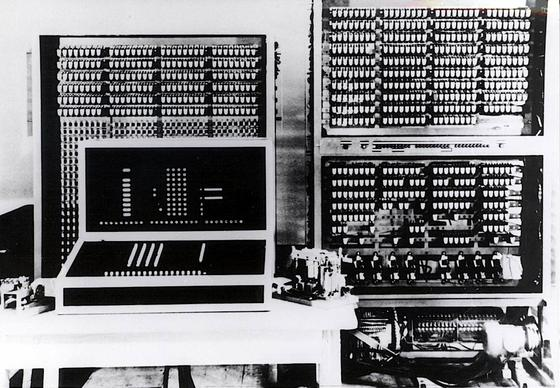
\includegraphics[width=0.7\textwidth]{Zuse_Z3.jpg}
  \caption{Zuse Z3 \cite{Zuse_Z3}}
  \label{fig:Zuse_Z3}
\end{figure}
Jedoch konnte dieser erste Computer, wie der Name bereits verrät (von eng. to compute = rechnen), die Daten nicht hauptsächlich speichern sondern verarbeiten. Und genau diese Datenverarbeitung ist es, die uns in den letzten Jahren so stark geprägt hat. Viele einfache Dinge, für die früher ein Mensch praktizieren musste, wird heute von einem Computer übernommen, der das ganze dann meistens auch noch viel schneller kann. Und genau diese Datenverarbeitung in Verbindung mit der Benutzerinteraktion steht bei unser Projektarbeit im Mittelpunkt. Das Ziel unseres Projekt ist es, dem Benutzer etwas beizubringen und das auf einem möglichst ertragreichem Weg. Das beizubringede wird auf Karten des Spiels "`Magic: The Gathering"'(Abbildung \ref{fig:Magiccard}) beschränkt.
\begin{figure}[htbp] 
  \centering
     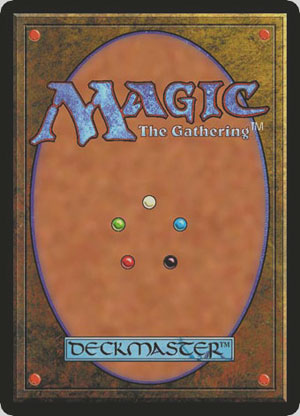
\includegraphics[width=0.4\textwidth]{Magiccard.jpg}
  \caption{Magickarte \cite{Magiccard}}
  \label{fig:Magiccard}
\end{figure}
Neben der Funktion mussten wir uns auch noch für eine Platform entscheiden, auf welcher unsere App verfügbar sein sollte. Da man jeder Zeit die Karten lernen können sollte, haben wir uns für eine mobile Android-App entschieden. Der Benutzer kann über ein Menu entscheiden, welche Karten er lernen will. Dann kann er über eine Lernfunktion die Karten lernen. Wie oben schon angeprochen, steht die Datenverarbeitung im Mittelpunkt. Deshalb speichern wir ab, ob der Benutzer die Karte gekonnt hat oder nicht. Falls ja, sollte die Karte in nächster Zukunft nicht noch einmal erscheinen, falls nein, sollte sie in naher Zukunft wieder erscheinen. Insofern kann man den maximalen Lernerfolg erreichen, da gezielt die Karten abgefragt werden, die noch nicht richtig sitzen. Ausserdem werden Daten auf zwei verschiedene Arten gespeichert: Einmal auf der App selbst und dann sollten diese auch noch ins Gedächniss des Benutzers gelangen. Natürlich sollte die App nicht nur funktionieren sondern auch noch ansprechend Aussehen und Benutzerfreundlich sein. Aber genau das ist es, was unsere App ausmachen soll: "`Magic2Brain"'

\newpage

%----------------------------------------------------------------------------------------
%	Theoretische Grundlagen
%----------------------------------------------------------------------------------------

\section{Theoretische Grundlagen} % Major section

In diesem Teil werden alle theoretischen Informationen gegeben, die man für das Verständniss des ganzen Projektes braucht. Nach dieser Einführung sollte man in der Lage sein, den Quellcode im Anhang zu verstehen. Da es jedoch sehr viel Übung erfordert, einen Quellcode zu lesen und zu verstehen, ist es naheliegend, dass der Quellcode nicht verstanden wird. In der Einführung wird grob angeschaut, wie man überhaupt vom Quellcode zur App kommt, im zweiten Teil wird erklährt, wie Daten jeglicher Art als Zahlen in einem Computer abgespeichert werden, im dritten Teil gibt es eine Einführung in die Programmiersprache Java und im letzten Teil werden dann noch ein paar spezifische Informationen in bezug auf Java gegeben, die für die Erstellung einer App gebraucht werden und die Software "`Android Studio"' wird erklährt.

\subsection{Einführung}
\subsubsection{Die IDE}
Die IDE (eng. integrated development environment) oder auf Deutsch die Entwicklungsumgebung ist der Ort, an dem die meisten Programmierer arbeiten. Sie bietet alle wichtigen Werkzeuge, die man zum entwickeln von Software benötigt (Editor mit Color Highlighting, Compiler, Debugger, Dateibrowser etc.). Auf einige Begriffe wird später noch genauer eingegangen. In unserem Falle heisst die Entwicklungsumgebung übrigens Android Studio. In der Entwicklungsumgebung findet die ganze Entwicklung einer Software statt. Der wichtigste Bereich davon ist der Editor. Dort wird der ganze Quellcode hingeschriben und dank Color Highlighting werden die wichtigen Komponenten (Kontrollstrukturen, Variablen, Kommentare etc. siehe Abschnitt 2.3 Grundlagen von Java) mit Farbe hervorgehoben (Abbildung \ref{fig:Colorhighlighting}).
\begin{figure}[htbp] 
  \centering
     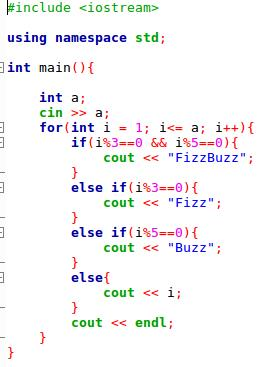
\includegraphics[width=0.3\textwidth]{CodeColor.jpg}
     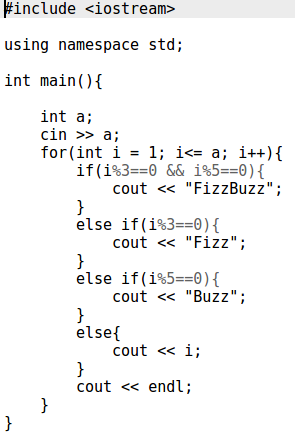
\includegraphics[width=0.3\textwidth]{CodeWithoutColor.png}
  \caption{Beispiel mit und ohne Farbhervorhebung \cite{Colorhighlighting}}
  \label{fig:Colorhighlighting}
\end{figure}
Das ist sehr wichtig, da man ansonsten schnell den Überblick verloren hat. Natürlich gibt es nicht nur eine IDE sondern ganz viele. Welche man davon benutzt ist jedem selbst überlassen. Es gibt auch Entwickler, die es bevorzugen, ohne eine IDE zu arbeiten. Zwar kann man dann alles selbst so gestallten wie es einem passt, es macht aber alles viel komplizierter ist besonders für neu beginnende Programmierer nicht empfehlenswert.

\subsubsection{Der Compiler}
Leider versteht der Computer nichts von dem, was wir in den Quellcode schreiben, alles was er versteht besteht aus Nullen und Einsen (mehr darüber im Abschnitt 2.2). Deshalb muss der für uns verständliche Quellcode in Maschinencode übersetzt werden. Dies geschieht mit dem so gennanten "`Compiler"' (eng. to compile = zusammentragen). Meistens ist dieser bereits in der IDE enthalten und auf Knopfdruck abrufbar. 

\subsubsection{Der Debugger}
Der Debugger ist sehr eng mit dem Compiler verbunden. Meistens schafft man es nähmlich nicht, auf Anhieb einen Fehlerlosen Code zu schreiben. Es passiert extrem schnell, dass irgendwo ein "`;"' oder eine Kontrollstruktur falsch geschrieben wurde (mehr dazu im Abschnitt 2.3). Deshalb ist es sehr wichtig, dass man den Fehler findet. Wenn man jetzt aber Quellcode von 500 Zeilen geschrieben hat, wäre es doch sehr mühsam, wenn man nur wüsste, dass man einen Fehler hat. Genau dafür ist der Debugger. Ist aus dem englischen Wort "`Bug"' entstanden, was so viel wie Käfer heisst, im Programmieren aber als Synonym zu Fehler verwendet wird. Dementprechend könnte man also Debugger als "`Entfehlerer"' oder verdeutscht als "`Fehlersuchprogramm"' bezeichnen. Meistens wird er aber einfach Debugger gennant. Offenbar ist der Debugger dazu in der Lage, die Programmierfehler zu finden. Er findet aber leider nur Syntaxfehler und keine, die den gewünschten Programmoutput betreffen. Man kann sich das so vorstellen: In Microsoft Word werden auch Rechtschreibefehler angezeigt, trotzdem kann man Sätze bilden die entweder keinen Sinn ergeben oder etwas anderes Aussagen, als gewünscht. Aber der Programmieraltag ohne Debugger wäre fast unvorstellbar, da man die meisten Fehler nicht so einfach sieht wie ein falsch geschriebenes Wort. Es gibt verschiedene Arten von Debugger. Die meisten zeigen einem die Fehler erst an, wenn man den Quellcode zu komplieren versucht, es gibt aber auch solche, die das in Echtzeit machen, so wie Microsoft Word Rechtschreibefehler anzeigt. 

\subsubsection{Die Programmiersprache}
Eine Programmiersprache kann man sich am einfachsten wie eine richtige Sprache vorstellen. Sie bildet den Grundbaustein des Programmierens. Bevor man dem Computer etwas  beibringen kann, muss man eine solche lernen. Jede Programmiersprache hat seine eigene Syntax, trotzdem sind sie meistens ähnlich aufgebaut. Sobald man also eine Programmiersprache gelernt hat, fällt es einem einfach, eine nächste zu lernen. Man muss sich das so vorstellen: Nachdem man gelernt hat, wie Windows XP funktioniert, hat man nicht mehr so grosse Schwierigkeiten, zu lernen wie Windows 7 oder Windows 8 funktioniert. Meistens haben die Programmiersprachen verschiedene Anwendungsbereiche: Wird z. B. JavaScript und PHP meist nur in Webanwendungen verwendet, wird C++ wegen seiner Geschwindigkeit meist in Systemanwendungen gebraucht oder Java für Geräte wie Drucker oder eben Androidapplikationen, ausserdem ist das berühmte Computerspiel "`Minecraft"' in Java geschrieben.
\subsection{Vom Binärcode zum Bild}
In diesem Teil geht es darum zu verstehen, wie ein Computer komplexe Informationen wie Bilder speichern kann. Dazu geht man zuerst von Binärcode (z.B. 01110110101001) aus und arbeitet sich dann hoch. Zwar ist dieses Thema nicht unbedingt notwendig, um unser Projekt nachvollziehen zu können, aber es hilft dabei, sich die Datenspeicherung besser vorstellen zu können, was auf jeden Fall sinnvoll ist, da ja die Datenspeicherung eines unserer Kernthemen ist. Ausserdem kann man dann auch die Datentypen in Java besser verstehen (Abschnitt 2.3).
\subsubsection{Vom Binärcode zur Zahl}
Die kleinste Speichereinheit eines Computers ist das Bit. Man sollte das Bit aber auf keinen Fall mit dem Byte verwechseln. Das Byte beinhalted nämlich acht Bits und ist dadurch viel grösser als das Bit. Man kann sich das Bit als Schalter vorstellen: Entweder ist er an oder er ist aus. Es gibt genau diese 2 Zustände. Mit der 1 bezeichnet man den angeschalteten Zustand und mit 0 den ausgeschalteten. Wenn man jetzt zwei Schalter nimmt dann gibt es bereits 4 verschiedene Schalterzustände: 00, 01, 10 und 11. Wenn wir nun $N$ Schalter anneinander reihen haben wir dementsprechend dann auch $2^N$ verschiedene Schalterzustände. Wenn wir jetzt jeden dieser Schalterzustände einer Zahl zuordnen, kann man je nach Schalteranzahl beliebig grosse Zahlen abspeichern. Jedoch wurden Zahlen nicht willkürich irgendeiner Schalterkombination zugeordnet sondern es gibt ein gewisses System dahinter, damit man die Zahlen nachher auch miteinander verrechnet werden können. Dieses System nenn man das binäre Zahlensystem. Es ist nicht wie unser dezimales Zahlensystem auf zehn ausgerichted sondern auf zwei. Um die Zahlen schreiben können, muss aber zuerst deffiniert werden, wie viele Bits gross eine Zahl ist. Diese Definition wird hier der Einfachheit halber auf 4 Bits gesetzt. Wie auch in unserem Zahlensystem wird die Zahl 0 als 0 dargestellt. Weil aber 4 Bits zur Verfügung stehen und nicht nur eines, müssen wir auch den anderen 3 einen Zustand geben, also auch 0. Dann sieh die Zahl 0 also binär dargestellt so aus: 0000. Auch die Zahl 1 ist noch eifach darzustellen: 0001. Wenn aber die Zahl 2 geschrieben werden soll, wird es bisschen komplizierter. Wir können nämlich den ersten Schalter nicht auf auf 2 Stellen. Die Antwort ist aber eigentlich ganz einfach: Wie in unserem dezimalen Zahlensystem nach der Zahl 9 eine neue Stelle gebraucht wird, so wird es binär genau gleich nach der Zahl 1 gemacht. Deshalb wird die Zahl 2 also so geschrieben: 0010. In diesem System geht es weiter: \\
\\
\begin{tabular}{l|l|l|l|l|l|l|l|l|l|l}
Dezimal & 0 & 1 & 2 & 3 & 4 & 5 & 6 & 7 & 8 &  ...\\ \hline
Binär & 0000 & 0001 & 0010 & 0011 & 0100 & 0101 & 0110 & 0111 & 1000 & ...\\
\end{tabular}  \\
\\
Dieses System gut zu kennen kann sehr nützlich sein. Wenn man die Zahlen nämlich noch ein bischen genauer analyziert, kann man feststellen, dass man die hinterste Stelle der binären Zahl immer angibt, ob der Zahl eine 1 addiert werden muss, die zweit hinterste dasselbe mit 2, der dritt hintersten mit 4. Bei jeder weiteren Stelle nach vorne nimmt die dazuzuaddierende Zahl um den Faktor 2 zu. Wenn man dieses System erkannt hat, kann man auch grosse binäre Zahlen in einer nützlichen Frist in eine dezimale übersetzten und umgekehrt. Hier ein Beispiel mit der achtstelligen Binärzahl 10100101:
\\
\begin{tabular}{l l l l l l l l l l l l l l l l l}
$1$ & & $0$ & &  $1$ & & $0$ & & $0$ & & $1$ & & $0$ & & $1$ & & \\
$ 128 $ &+& $0$ &+& $ 32$ &+& $0$ &+& $0$ &+& $ 4$ &+& $0$ &+& $1$ &=& $165$ \\ 
\end{tabular} \\
\\
Das hier vorgestellte binäre Zahlensystem ist jedoch stark vereinfacht, da sich in diesem nur Zahlen $\in \mathbb{N} $ darstellen lassen. Negative Zahlen und Gleitkommazahlen würden aber zu stark vom eigentlichen Thema abweichen. Wichtig ist nur, dass der Computer nur so gennante Maschienenzahlen abspeichern kann. Das heist die Zahlen müssen endlich gross sein und deshalb können periodische und irrationale Zahlen nicht genau abgespeichert werden.
\subsubsection{Grundoperatoren bei binären Zahlen}
Wenn man erst mal verstanden hat, wie das binäre Zahlensystem funktioniert, dann sind die Grundoperationen sehr einfach. Sie lassen ganz einfach mit den schriftlichen Operationen berechnen. Als Beispiel werden 5 Bit grosse Zahlen genommen: Die Zahl 6 (00110) und die Zahl 3(00011).
\paragraph{Addition}
\begin{tabular}{llllll}
&0&0&1&1&0 \\
+&0&0&0&1&1 \\ \hline
&0&1&0&0&1
\end{tabular}
\paragraph{Subtraktion}
\begin{tabular}{llllll}
&0&0&1&1&0 \\
-&0&0&0&1&1 \\ \hline
&0&0&0&1&1
\end{tabular}
\paragraph{Multiplikation}
\begin{tabular}{lllllllllll}
0&0&1&1&0& $\cdot$ &0&0&0&1&1 \\ \hline
&&&&&&0&1&1&0&0 \\
&&&&&&0&0&1&1&0 \\ \hline
&&&&&&1&0&0&1&0
\end{tabular}
\paragraph{Division}
\begin{tabular}{lllllllllll l}
0&0&1&1&0& : &0&0&0&1&1 & = 0 0 0 1 0 \\ \hline
 & &1&1& & &&&&&& \\ \cline{3-4}
 & &0&0&0& &&&&&& \\ 
\end{tabular}
\subsubsection{Von der Zahl zur Text}
Mit dem Wissen, wie Zahlen binär gespeichert werden, kann man dann sehr eifach verstehen, wie Texte abgespeichert werden. Im Grundsatz ist es nur eine willkürliche Zuordnung von Zeichen zu einer Zahl. Es gibt verschiedene Zuordnungen, die wichtigsten hierbei sind ASCII (American Standart Code for Information Interchange) und UTF-8(Universal Character Set Transformation Format). ASCII hierbei speichert jegliche Zeichen in 7 Bits ab und kann aber nur 128 verschiedene Zeichen speichern. Zum Beispiel würde man das Wort Haus so kodieren: 72 97 117 115. Wenn man diese Zahlen auch noch in Bits übersetzt, hat man die exakte Kodierung, wie sie auch auf dem Computer abgespeichert würde: 1001000110000111101011110011(siehe Abbildung \ref{fig:ASCII})
\begin{figure}[htbp] 
  \centering
     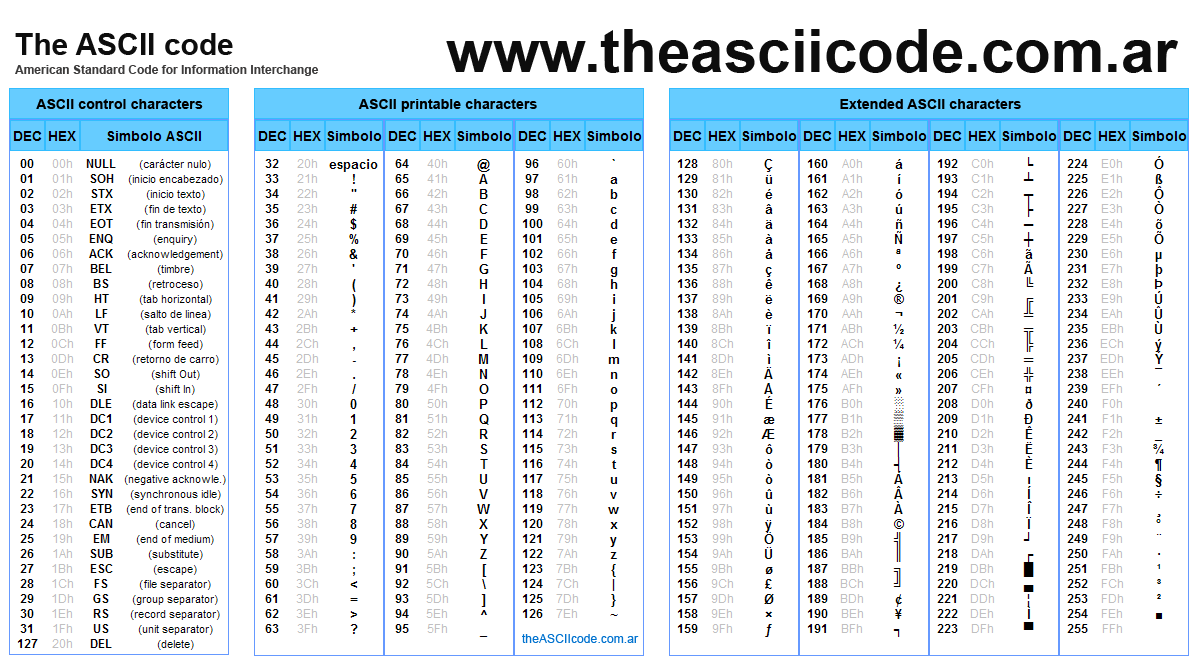
\includegraphics[width=1\textwidth]{ASCII.png}
  \caption{ASCII Tabelle \cite{ASCII}}
  \label{fig:ASCII}
\end{figure}
Dadruch werden viele sprachspezifischen Zeichen wie die deutschen Umlaute nicht abspeicherbar. Deshalb wird ASCII heutzutage auch meistens nicht mehr gebraucht. UTF-8 ist hierbei viel nützlicher, aber auch komplizierter. Es kann jegliche Spezialzeichen jeder Sprache abspeichern. UTF speichert die einfachen ASCII Zeichen in 8 Bits ab, das erst hinzugekommene Bit speichert ab, ob es sich bei dem Zeichen um ein ASCII Zeichen handelt oder nicht. Falls ja, können die restlichen sieben Bits wie ein ASCII Zeichen interpretiert werden. Ansonsten folgen nicht nur 7 Bits sondern wieder abhängig von der nächsten Zeichenfolge bis zu 31 weitere Bits (im ganzen dann 4 Bytes). Die deutschen Umlaute brauchen zum Beispiel 2 Bytes Speicherplatz. UTF-8 ist heutzutage der meist verbreitete Zeichensatz im Internet (im November 2016 benutzen rund 88\% aller Webseiten UTF-8). \cite{UTF-8} Ein weiterer heutezutage sehr verbreiteter Zeichensatz ist Unicode, auf diesen wird hier aber nicht weiter eingegangen.
\subsubsection{Von der Zahl zur Farbe}
Um Bilder abspeichern zu können, muss man zuerst einmal wissen, wie Farben abgespeichert werden. Die meist verbreitete Methode für das Abspeichern von Farben ist RGB (eng. Red Green Blue). Der Name spricht für sich, nacheinander wird die Menge der Farbe Rot, Grün und Blau in einer Skala von 0 bis 255 angegeben. Aber auch die Farben werden in einem unüblichen Zahlensystem dargestellt: im Hexadezimalen. Dieses basiert nicht wie das binäre auf 2 und das dezimale auf 10, sondern auf 16. Da in unserem Zahlensystem keine Ziffer für 10-15 existieren, hat man dier ersten Buchstaben des Alphabetes genommen. 10 wäre also "`A"' und 15 wäre "`F"' hexadezimal geschrieben. \textbf{Achtung: Wegen diesem System ist die hexadezimale 10 nicht dasselbe wir die dezimale 10 sondern 16.} 255 wäre dementsprechend "`FF"' hexadezimal geschrieben und somit die grösste hexadezimale Zahl, die mit zwei Ziffern geschrieben werden kann. Das ist natürlich kein Zufall sondern extra so gewählt. Um eine hexadezimale Zahl zu kennzeichnen, benutzt man in der Regel den Präfix 0x. Ein RGB wert besteht also aus drei zwei stelligen hexadezimalen Zahlen. Meistens wird bei RGB-Farben ein \# als Präfix verwendet anstatt des hexadezimal üblichen 0x. Auch noch wichtig anzumerken ist, dass das RGB-System ein additiver Farbraum ist. Das heisst also wenn man die volle Farbstärke aller Farben Rot, Grün und Blau verwendet, erhält man weiss. Hier nun eine Tabelle mit den wichtigsten Farben und dem dazugehörigen hexadezimalen Wert. \\
\\
\begin{tabular}{|l|l|l|l|}
\hline
Rot & Grün & Blau & Weiss \\ \hline
\#FF0000  & \#00FF00 & \#0000FF & \#FFFFFF \\ \hline
Schwarz & Gelb & Magenta & Cyan \\ \hline
\#000000 & \#FFFF00 & \#FF00FF & \#00FFFF \\ \hline
\end{tabular} \\
\\
Übrigens ist es auch kein Zufall, dass die Farben hexadezimal dargestellt werden und nicht dezimal. Ein System, welches auf zehn basieren würde, hätte immer ein gewissen Datenverlust, da man um 10 darstellen zu können 4 Bits braucht. Mit 4 Bits lassen sich aber Zahlen bis 16 darstellen. Um also mit demselben Speicherbedarf die maximale Speicherausnutzung zu erreichen, hat man sich für ein hexadezimales System entschieden. Es gibt auch hier nicht nur ein System, ein weiteres sehr wichtiges Farbsystem ist das "`CMYK"', welches vor allem für Drücker verwendet wird. Dieses System ist im Gegensatz zum RGB-Farbsystem ein subtraktives. Der Name steht für Cyan Magenta Yellow Key. Auch wie im RGB-Farbsystem werden mit Cyan, Magenta und Gelb die Menge der Farben dargestellt. Das CMYK-Farbsystem besitzt aber noch einen vierten Wert: Den Schwarzanteil (hier mit K für Key angegeben um nicht mit B für Black um eine Verwechslungsgefahr mit Blue zu vermeiden).
\subsubsection{Von der Farbe zum Bild}
Nun sollten alle Grundlagen vorhanden sein, um zu verstehen, wie ein Bild gespeichert werden kann. Hier wird zuerst von einem total unkomprimierten Bild ausgegange, das mit RGB Farben ausgestattet ist. Digitale Bilder können in zwei Gruppen unterteilt werden: Rastergrafiken und Vektorgrafiken. Zuerst wir ersteres angeschaut. Ein Computerbildschirm ist bekanntlicherweise aus einzelnen Pixeln aufgebaut. Jedes dieser Pixel funktioniert eigenstädnig und kann eine belibige Farbe anzeigen. Heutzutage ist das wohl am weitesten Verbreitete Bildschirmformat das Full-HD mit 1920x1080 Pixeln. In einem völlig unkomprimierten Bild wird also für jedes Bild seine eigene Farbe gespeichert und schon hat man sein Bild abgespeichert. Wir aber aus dem letzt Kapitel über Farben bekannt ist, werden die Farben üblicherweise mit RGB abgespeichert. Wenn man nun bedenkt, wie diese Zahlen binär aufgebaut werden, kommt man für jede hexadezimale Stelle auf 4 Bits, die gebraucht werden. Weil eine normale RGB-Farbe aus 6 hexadezimalen Zahlen bestehen, heisst das wiederum, dass eine RGB-Farbe mit 24 Bits geschriben werden kann, was das gleiche wie 3 Bytes ist. Um also ein Bild abzuspeichern, werden $1920 \cot 1080 \cdot 3=6220800$ Bytes $ \approx  6.5$ Megabytes. Das ist bereits eine sehr grosse Datenmenge. Für Qualitativ hochwertige Bilder ist die Auflösung aber oftmals grösser und die Farbe genauer, wodurch der Bildspeicherplatzbedarf nochmals enorm wachsen würde. Wenn man jetzt sogar ein Video mit 60 FPS (eng. Frames Per Second = Bilder pro Sekunde) mit dieser Datengrösse des errechnetetn Bildes mit 6.5MB  speichern würde, würde man für jede Sekunde 390MB verbrauchen. Dadurch wäre also ein Film mit einer durschnittlichen Länge von 1.5h 2.106TB gross, also grösser als die meisten Speicher eines Computers. Die Realität sieht aber ganz anders aus: Um Speicherplatz zu optimieren werden erstens bei Bildern komprimierungen angewendet, welche über komplexe Algorithmen die Bilder so abspeichern, dass diese viel weniger Speicherplatz einnehmen. Ausserdem speichern Videos nicht jedes Bild neu sondern nur dessen Veränderung. So kommt man dann auf eine etwa 1000 mal kleinere Speichergrösse. Bei Bildkompression unterscheidet man übrigens auch zwischen verlustbehafteten Kompressionen und verlustfreien. Bekannte verlustfreie Kompressionen sind zum Beispiel TIFF und PNG und bekannte verlustbehaftete JPEG und GIF \cite{Dateiformate}. Jedes Dateiformat hat aber seine eigenen Vorteile und Nachteile und je nach Zweck solle man sich überlegen, welches davon am meisten Sinn macht. Wie Anfangs erwähnt gibt es aber auch noch die Vektorgrafik. Die Vektorgrafik speichert keine Informationen über einzelne Pixel sondern es speichert zum Beispiel eine Linie oder ein Kreis mit einer Funktion. Der Vorteil einer Vektorgrafik ist, dass man diese frei skalieren kann, ohne dass man eine Qualitätseinbusse hat. Meistens sind Firmenlogos und Ähnliches mit einer Vektorgrafik geschrieben.
\subsection{Grundlagen von Java}

\subsection{Android Studio}
Android Studio ist eine vom Andoid Open Source Project (kurz: AOSP) entwickelte Entwicklungsumgebung auf der basis von IntelliJ, dabei sollte beachtet werden, dass Android Studio im gegensatz zu Android OS
proprietären Code beinhaltet und somit weder open source ist, noch ohne erlaubnis durch dritte weiterverbreitet werden darf.
IntelliJ ist eine bereits bestehende propietäre Entwicklungsumgebung für Java (bzw. JVM) und Android, des weiteren kann eine Lizenz für Firmen und Webentwickler erworben werden.
Im grunde wurde Android Studio mit der hinsicht auf Applikationsentwicklung auf dem Android OS erstellt. Es beinhaltet von Haus aus notwendige, aber auch arbeitserleichternde Komponenten, wie
einen Gradle-Compiler (Notwendig) oder einen Android-Empulator (Erleichtert das testen der App auf einem Computer).\\

%FIXME rechtschreibung
Gradle ist ein Open Source Build-Tool, was im Grunde über den eigentlichen Compiler-Prgogrammen eine oberste Schicht in der Compiler-Toolchain bildet. Daher verkörpert Gradle mehrere separate aufgaben in sich und vereinfacht das kompillieren von Android Apps enorm.
Die Kernkompnenten von Gradle sind
\begin{itemize}
\item \textbf{Linker, bzw. Zusammentragen von zusätzlichen Paketen und androidspezifischen Dateien, die für das Kompillieren erforderlich sind.} Dabei werden Pakete resp. Bibliotheken von den Quellen runtergeladen, 
die man zu der Quellenliste hinzugefügt hat. Dies erleichtert das Hinzufügen von Bibliotheken wie z.B. einer Bibliothek zum herunterladen und anzeigen von Bildern, da man nur die Downloadadresse angeben muss
und sich nicht mehr um das Einbinden der Bibliothek in sein Applikationsprojekt kümmern muss.

\item \textbf{Debugger} Wie bereits beschrieben liest sich der Debugger noch vor dem Precompiler den Code durch und macht den Programmierer auf allfällige Fehler oder verbesserungen aufmerksam.

\item \textbf{Precompiler} Der Precompiler ist ein Kernbestandteil der Compiler-Toolchain. Eine Toolchain ist eine Ansammlung von Programmen, die einem helfen aus geschriebenen Code und Assets ein lauffähiges
Programm zu erstellen. Er liest jede Datei durch und bereitet sie auf die nachfolgenden Verarbeitungsprozesse vor, indem er unter anderem Kommentare entfernt, nichtgenutzte Funktionen und Variabeln entfernt, Makros ersetzt und durch die \verb include -Kontrollzequenz eingebundene Dateien einfügt. Die heutigen Precompiler bleiben aber meist nicht nur bei ihren Kernaufgaben, sondern versuchen auch den Code so weit zu verbessern,
dass er nach dem Kompilliervorgang eine geringere Laufzeit und Speicheraulastung aufweist. Dabei ist aber zu beachten dass Compiler und Precompiler sehr eng miteinander zusammenarbeiten.

\item \textbf{Compiler} Der Compiler ist wohl das bekannteste Programm aus einer klassischen Toolchain. Er sogt dafür, dass die von dem Precompiler aufbereiteten Dateien in Maschinensprache übersetzt werden.
Wie bereits in der Einleitung erwähnt rechnet der Computer Binär. Daher ist eine Datei nichts anderes als eine lange Zahl. Je nach Prozessortyp wird auch eine Zahl anders verarbeitet. Dieser unterschied liegt in der verarbeitung von Kontrollsequenzen. In diesem trivialen Beispiel soll verdeutlicht werden, wie zwei verschiedene Prozessoren ein und die selbe Zahl anders interpretieren: Der Befehl für eine additionsoperation wird hier durch 11100010 repräsentiert. Im Prozessortyp A löst dies wie gewollt eine Addition aus, hingegen im Prozessortyp B werden die nachfolgenden Bits in den Zwischenspeicher kopiert. Prozessoren haben also auch ihre eigene Sprache, die sich durch ihre Herstellung ergibt. Diese Sprache wird \textit{Befehlssatz} genannt, wohingegen der Prozessortyp \textit{Architektur} genannt wird. Jede Prozessorarchitektur hat ihren eigenen Compiler.
Im Fall von Android haben sich drei Architekturen etabiliert: armeabi-v7, Intel x86 und AMD64. Die App wird also in mehrere Sprachen übersetzt bevor sie ausgeleifert wird.
\end{itemize}

\newpage

\begin{figure}[htbp] 
  \centering
     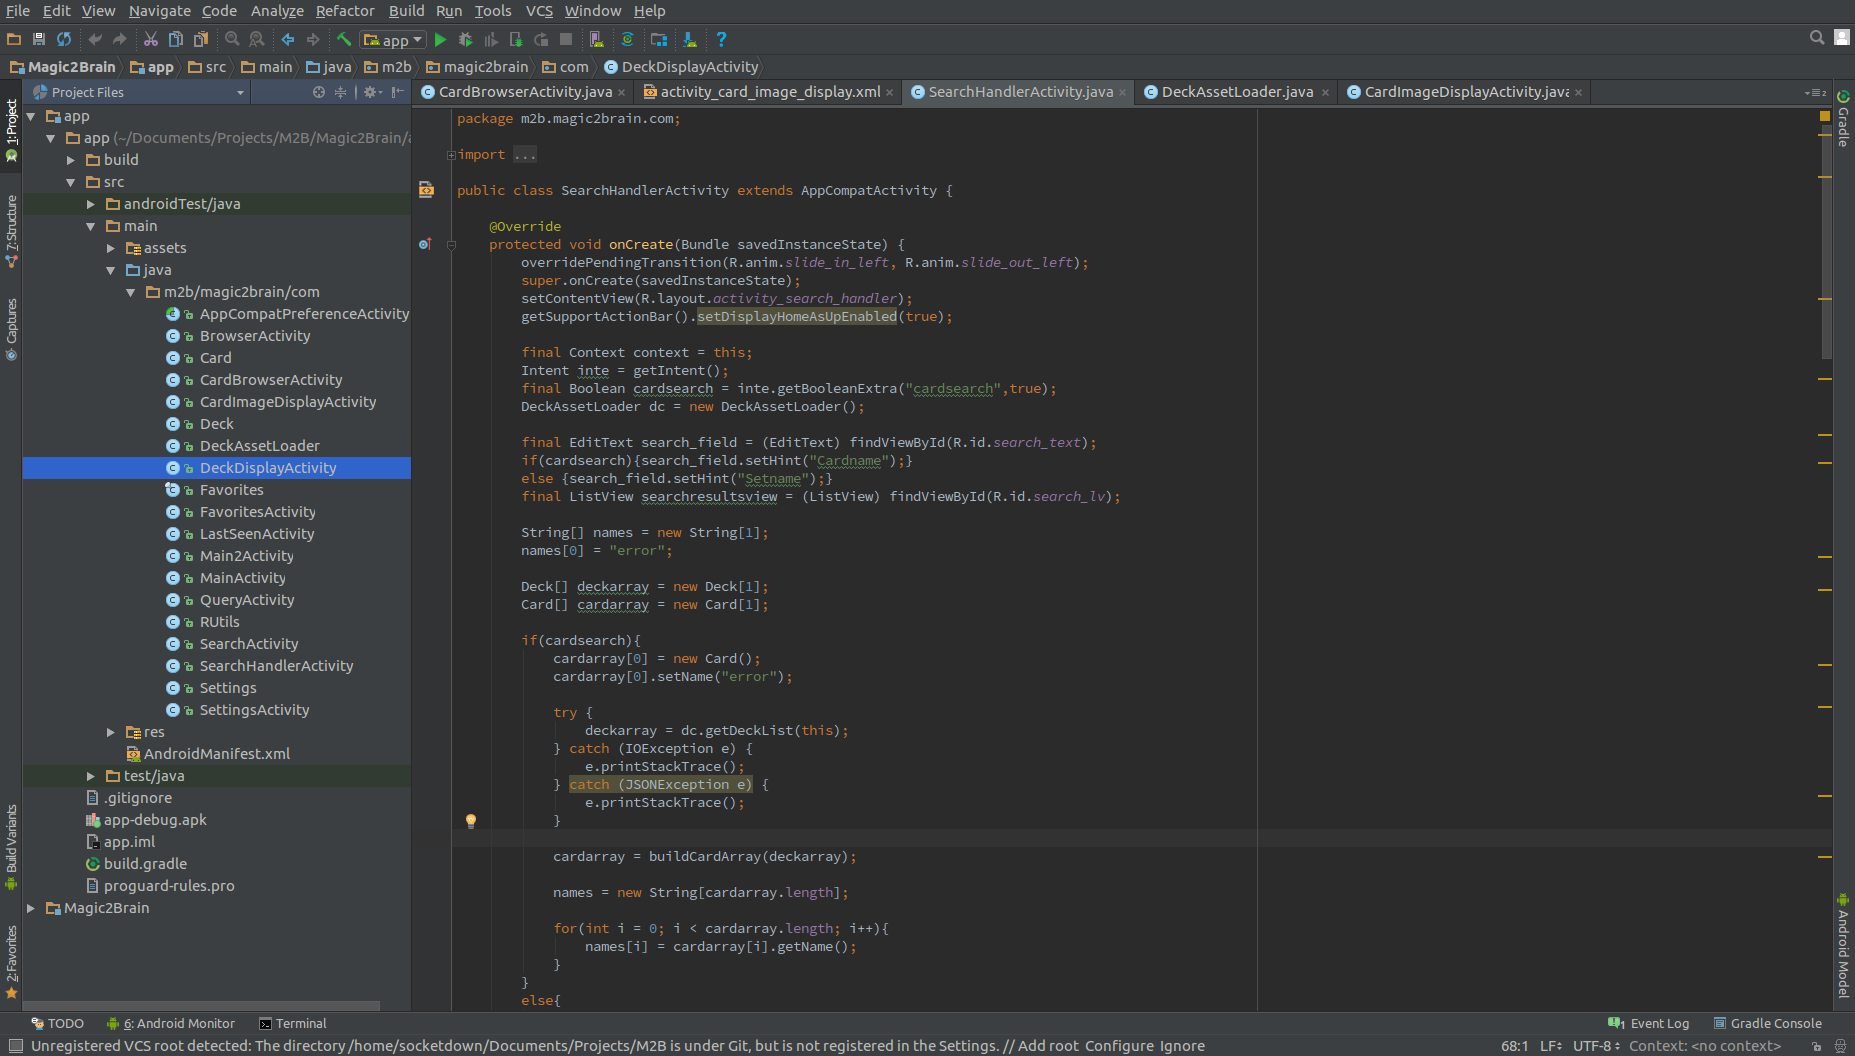
\includegraphics[width=1\textwidth]{AndroidStudio_GUI.png}
  \caption{Android Studio Benutzeroberfläche \cite{ASGUI}}
  \label{fig:Android Studio GUI}
\end{figure}
Die Grafische Benutzeroberfläche ist das Wichtigste an einer IDE. Sie erleichtert dem Entwickler die Navigation durch seinen Code in Form von Farbmarkierungen (Rechts) und Dateibrowser (Links).
Die Toolbar von Android Studio (Oben) ist mit wichtigen Shortcuts, wie z.B. Kompillierung starten, Emulator starten und Android SDK aktualisieren, gefüllt.
Der Editor von Android Studio erlaubt eine automatische Vervollständigung mit Alt+Enter. Mitunter sind auch schon fertige Vorlagen für Activities in Android Studio verfügbar, die auf Knopfdruck in das Projekt kopiert werden und gleichzeitig für die Kompillierung registirert werden. Der Dateibrowser erlaubt es zwischen Quellcode-Dateien zu wechseln und diese zur Bearbeitung zu öffnen. Zusätzlich sind funktionen zum importieren von Dateien oder Assets vorhanden. Selbstverständlich kann dies auch manuell geschehen, indem man in einem beliebigen Dateibrowser zu dem Assets resp. Res (kurz für \textit{Ressources - dt. Ressourcen} ) - Ordner, in dem man seine Dateien ablegen kann. Mit Assets sind hier nicht Immobilien oder Vermögen gemeint, sondern Dateien, die von der App benötigt werden um richtig zu funktionnieren. Dazu gehören Bilder, Musikdateien und generell alles was kein Quellcode ist. Der IDE kann man auch Plugins hinzufügen. Plugins sind kleine Programmerweiterungen, welche dynamisch dazugeladen oder wieder entfernt werden können. Bei der Entwicklung von Magic2Brain ist das Plugin "Asset Studio" besonders nützlich gewesen, da man mit ihm Icons nicht nur in den Ressourcenordner kopieren konnte, sonder diese gleich in allen auf Android gängigen Auflösungen abspeichern konnte. Normalerweise müsste das von Hand gemacht werden, was bei unseren ca. 20 Icons sehr zeitaufwändig gewesen wäre.
%TODO ASGUI fertigschreiben

\newpage

%----------------------------------------------------------------------------------------
%	Methode
%----------------------------------------------------------------------------------------

\section{Methode} % Major section

Es gibt mehrere Möglichkeiten eine Android App zu programmieren. Man kann ein Framework (z.B. "`LibGDX"') nutzen um mit einer vertrauten Programmiersprache und IDE eine App zu entwickeln. Google selbst bietet eine eigene IDE namens "`Android Studio"'. Wir entschieden uns anfangs mit Phonegap zu entwickeln.


\subsection{Die Arbeit mit Phonegap}
Phonegap ist mit dem Framework Cordova aufgebaut. Der Vorteil von Phonegap ist, dass es für das Design HTML nutzt. Wir sind vertraut mit HTML und können damit schnell relativ ansehnliche Benutzeroberflächen (kurz: GUI) erstellen. Als Programmiersprache nutzt Phonegap Javascript. Auch damit sind wir vertraut, da wir ein Semester lang damit gearbeitet haben. Wir konnten also direkt loslegen. Phonegap bietet zudem die Möglichkeit die App direkt auf dem Smartphone zu betrachten. Diese Funktion ist sehr praktisch, wenn man kurz was betrachten will. 

\subsection{Der Aufbau der App}
Wir wollten die Arbeit am Aufbau der App gleichmässig aufteilen. Wenn mehrere Personen an einem Projekt arbeiten, muss man dafür sorgen, dass keine Konflikte entstehen. Konflikte können entstehen, wenn z.B. mehrere Personen die gleiche Datei bearbeiten. Um dies zu verhindern wollten wir jede Seite der App in eine eigene Datei auslagern. Es sollte ein Menu geben, von wo aus man auf jede Seite zugreifen konnte. Dieses Menu musste am Anfang von einer Person erstellt werden. Danach konnten wir die einzelnen Seiten auf die Personen aufteilen und gleichzeitig Arbeiten, ohne dass Konflikte entstehen. Jede Seite sollte eine eigene Funktion haben. Z.B. gab es eine Seite für die Abfragen, eine Seite mit Favoriten etc. Mit einem Zurück-Knopf kommt man von jeder Seite zum Menu zurück.

\subsection{Der Wechsel zu "`Android Studio"'}
Wir haben viel Zeit damit verbracht mit Phonegap eine schöne Benutzeroberfläche zu erstellen. Als wir dann dazu kamen die Funktionalität zu programmieren, merkten wir was der Nachteil von Phonegap ist. Phonegap nutzt Javascript als Programmiersprache. Javascript ist asynchron. Das heisst, dass es nicht linear (Ein Befehl nach dem Anderen) ausgeführt wird, sondern die Befehle einer Funktion praktisch gleichzeitig ausführt. Dies ist super, wenn man Animationen erstellen will, aber wenn ein Befehl auf das Resultat von einem anderen Befehl aufbaut, gibt es viele Probleme. Man kann das Problem mit Workarounds lösen, aber dies ist einerseits möglicherweise stabil auf allen Geräten und andererseits ist es extrem aufwändig. Also fassten wir den Entschluss nochmals neu anzufangen, aber diesmal mit "`Android Studio"'. "`Android Studio"' nutzt Java als Programmiersprache. Auch mit dieser Programmiersprache kennen wir uns bestens aus. Dies vereinfachte die Entwicklung der Funktionalität um einiges. "`Android Studio"' nutzt für die GUI XML. XML ist von der Syntax her praktisch gleich wie HTML. Also mussten wir nicht viel umlernen. Bei XML gab es nur andere Elemente, welche wir lernen mussten. Etwas gewöhnungsbedürftig war die Verknüpfung zwischen XML und Java. Wir mussten lernen, wie man mit Java auf Elemente vom XML zugreift und diese verändert. Hinzu kam noch, dass wir uns mit dem Lebenszyklus einer App auseinandersetzen mussten. Bei Phonegap wurde das automatisch erledigt. Nach dem Lernen dieser Kleinigkeiten ging die Entwicklung viel schneller voran als bei Phonegap. Somit hat sich der Umstieg definitiv gelohnt. 

\newpage

%----------------------------------------------------------------------------------------
%	Darstellung und Ergebnisse
%----------------------------------------------------------------------------------------

\section{Darstellung der Ergebnisse} % Major section

Das Logo der App dient als Splashscreen (Abbildung \ref{fig:splashundmenu}). Nach dem Laden wird man von der Home-Seite begrüsst. Streift man mit dem Finger von Links nach Rechts oder klickt auf das Menü-Sandwich, öffnet sich ein Side-Menü. Das Side-Menü hat oben wieder das Logo und darunter zwei Texte ("`Magic 2 Brain"' und "`Your MTG learning companion"'). Unter dem befinden sich 7 Schaltflächen mit den Texten: "`Home"', "`Search"', "`Set Browser"', "`Quick Learn"', "`Favorites"', "`Recently Learned"' und "`Share"' (Abbildung \ref{fig:splashundmenu}).

\begin{figure}[htbp]
 \centering
    
\includegraphics[width=0.3\textwidth]{startup.jpg}
    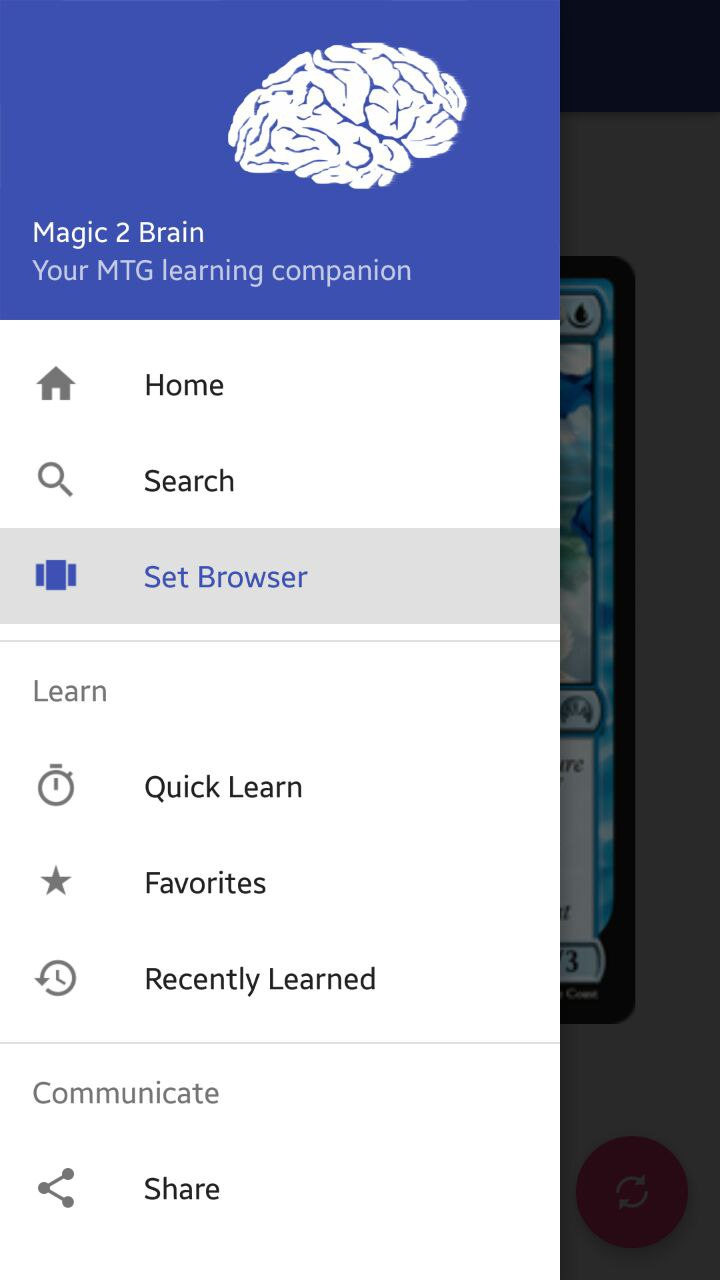
\includegraphics[width=0.3\textwidth]{sidemenu.jpg}
 \caption{Links: Der Splash-Screen, Rechts: Das Menü}
 \label{fig:splashundmenu}
\end{figure}

\subsection{Home}
Der Homescreen ist simpel aufgebaut. Ganz oben ist "`Magic2Brain"' geschrieben und direkt unter dem "`Random Card"'. Mitten auf dem Bildschirm ist eine zufällige Karte abgebildet. Mit einem Klick auf die Karte lässt sich diese vergrössern. Ganz unten rechts ist ein runder Knopf. Dieser ersetzt bei einem Klick die Karte mit einer anderen zufälligen Karte. (Abbildung \ref{fig:homemenu}).

\begin{figure}[htbp]
 \centering
    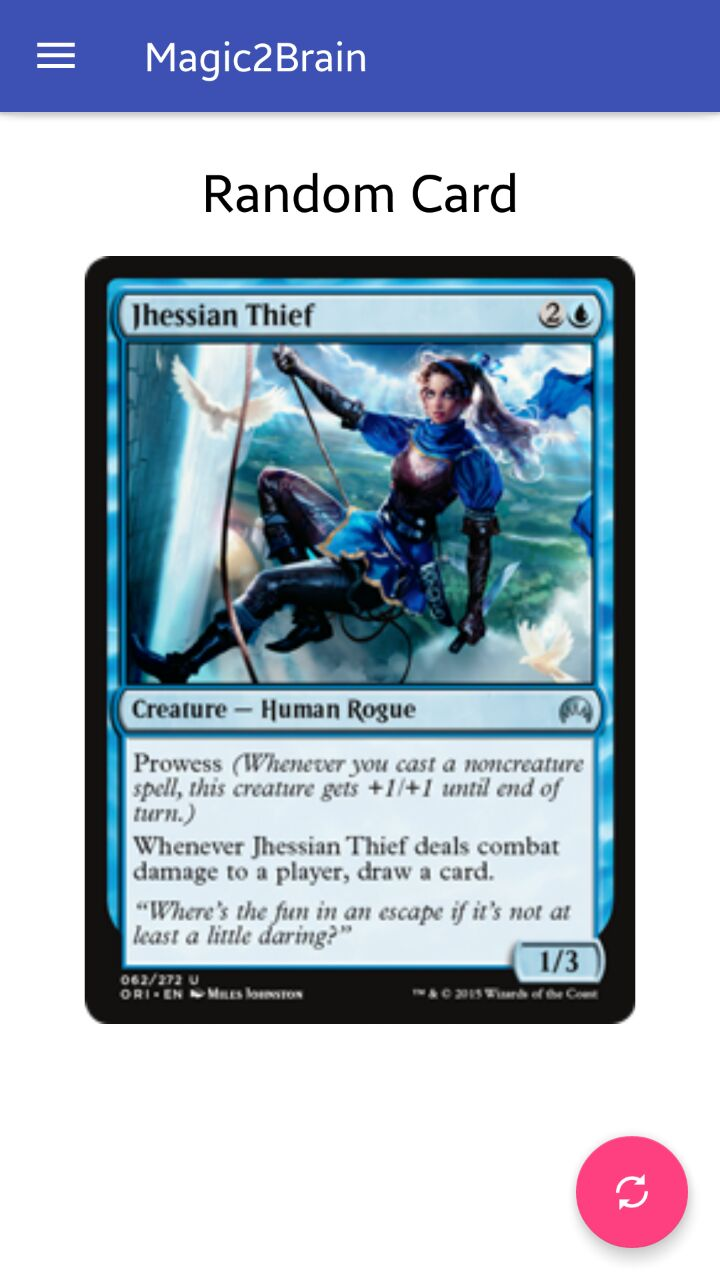
\includegraphics[width=0.3\textwidth]{home.jpg}
 \caption{Der Home-Screen \cite{Magiccard}}
 \label{fig:homemenu}
\end{figure}

\subsection{Search}
Wird auf "`Search"' gedrückt, kann ausgewählt werden, ob nach Karten oder Sets gesucht wird. Wählt man eine der beiden Optionen aus, wird man zu einer Ansicht mit einem Textfeld über einer Liste weitergeleitet. Tippt man etwas in das Textfeld ein, ändert sich die Liste und zeigt nur die Suchergebnisse an.

\subsection{Set Browser}
Der Set-Browser zeigt alle Sets in einer Liste an (Abbildung \ref{fig:setbrowser}). Drückt man auf ein Set, erscheint eine weitere Ansicht mit einer Liste. Diese Liste beinhaltet alle Karten vom ausgewählten Set. Navigiert man auf eine Karte, sieht man die Karte in einer Detailansicht. Bild, Text, Manakosten und der Name der Karte werden angezeigt (Abbildung \ref{fig:setbrowser}). Zudem hat man einen Knopf mit einem Herzen drauf. Betätigt man diesen, wird die Karte zu den Favoriten hinzugefügt.

\begin{figure}[htbp]
 \centering
    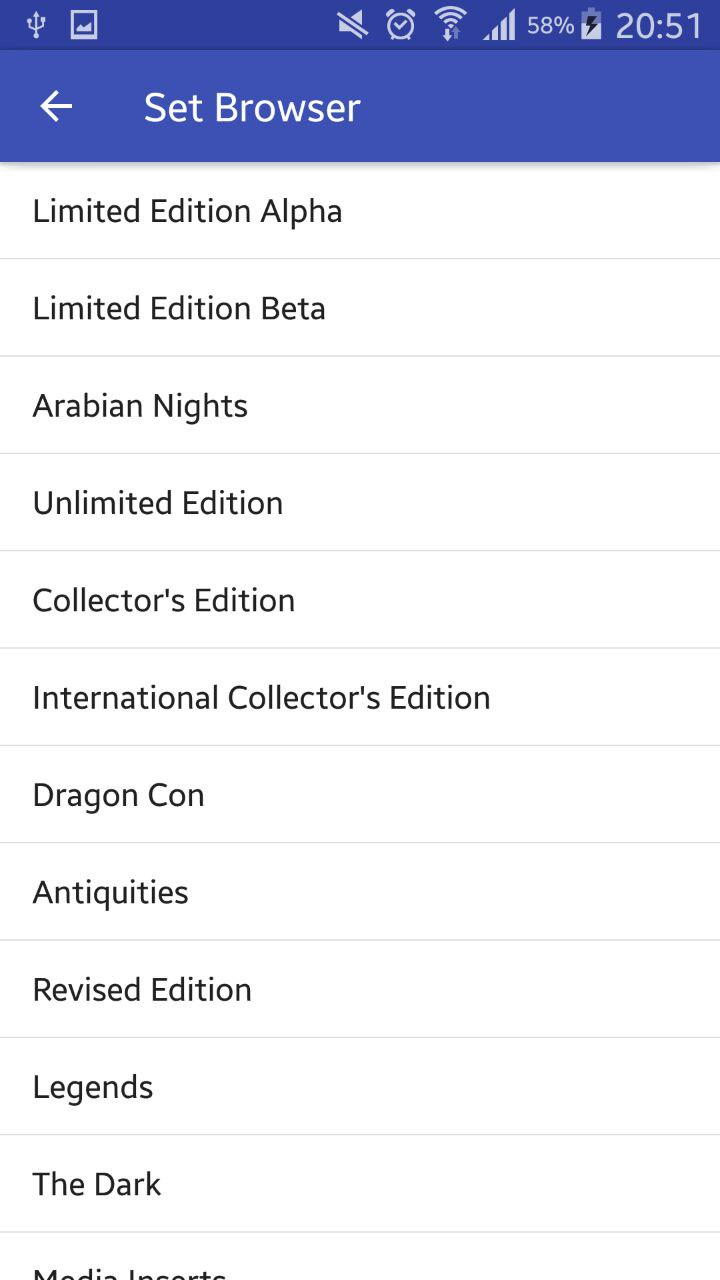
\includegraphics[width=0.3\textwidth]{setbrowser.jpg}
     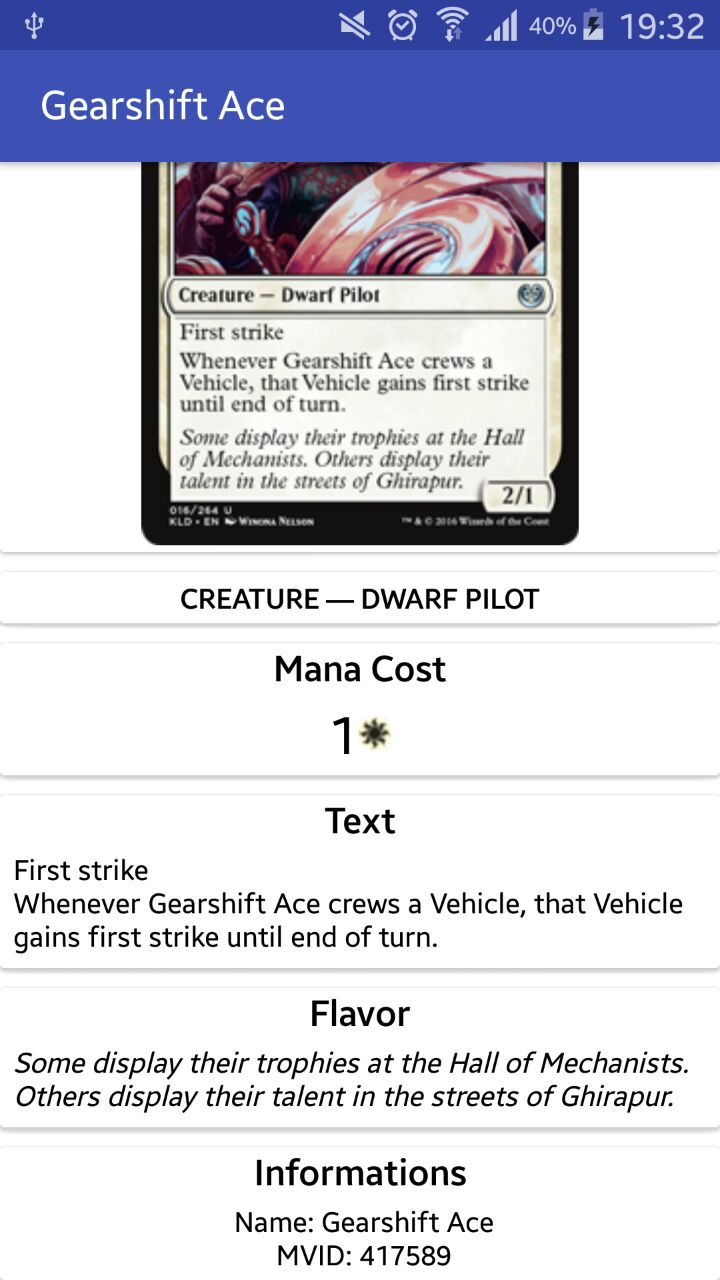
\includegraphics[width=0.3\textwidth]{cardview.jpg}
 \caption{Links: Der Set-Browser, Rechts: Die Karten-Ansicht \cite{Magiccard}}
 \label{fig:setbrowser}
\end{figure}

\subsection{Quick Learn}
"`Quick Learn"' startet eine Abfrage mit dem aktuellsten Set. In diesem Fall ist es Kaladesh. In der Mitte wird eine Karte vom Set gezeigt. Dabei ist der Text der Karte abgedeckt. Unterhalb der Karte befinden sich vier Schaltflächen mit verschiedenen Texten. Einer der Knöpfe enthält den Text der Karte. Drückt man die richtige Schaltfläche, wird kurz ein Haken auf die Karte projiziert, ansonsten ein Kreuz. Nach dieser Animation wird das Bild der Karte durch die nächste Karte im Set ersetzt. Die Schaltflächen ändern zudem ihren Text. Oben rechts befindet sich ein Menü-Sandwich. Bei dessen Betätigung sich ein Menü mit 3 Optionen öffnet: "`Query Lands"',"`Reverse query"' und "`Restart". Mit "`Query Lands"' kann man auswählen, ob die Länder auch abgefragt werden sollen. "`Reverse query" ändert den Abfragemodus. Im alternativen Modus ist der Name der Karte verdeckt. Unter der Karte befindet sich ein Textfeld, worin man den Namen der Karte eingeben soll. "`Restart" startet die ganze Abfrage neu (Abbildung \ref{fig:queryview}).

\begin{figure}[htbp]
 \centering
    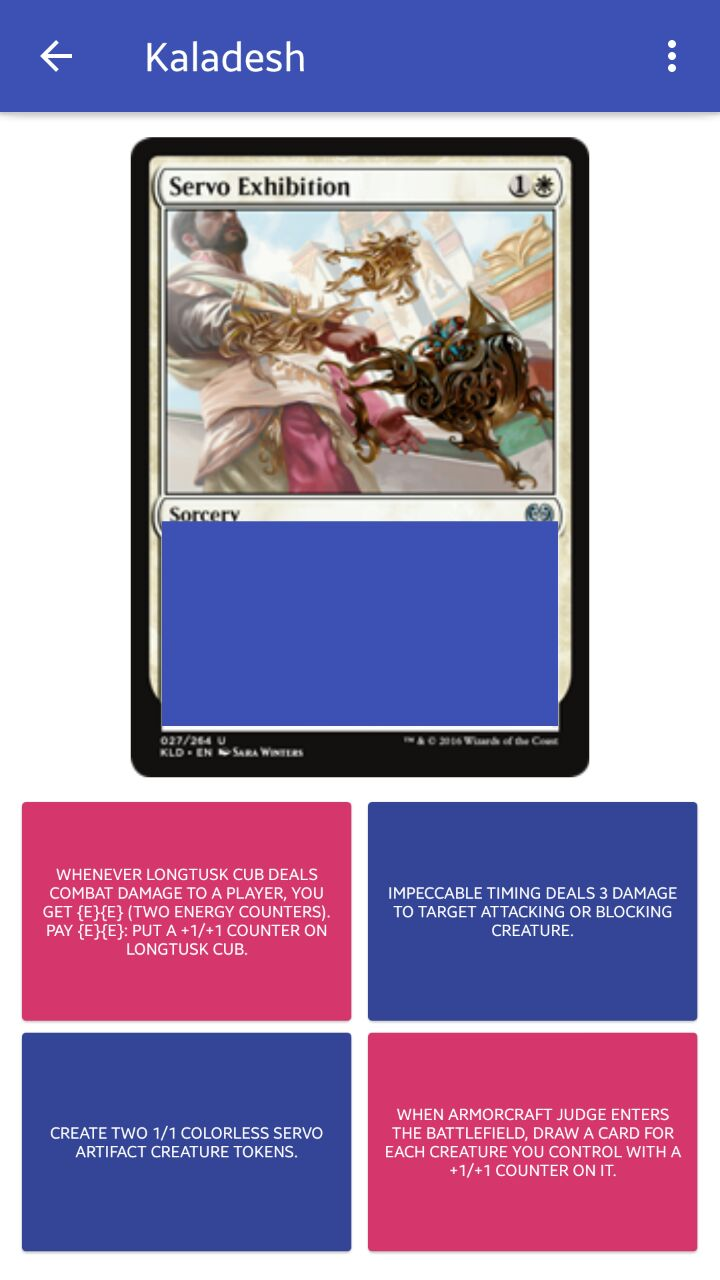
\includegraphics[width=0.3\textwidth]{query.jpg}
 \caption{Die Abfrage eines Sets \cite{Magiccard}}
 \label{fig:queryview}
\end{figure}

\subsection{Favorites}
Wechselt man auf den Reiter Favoriten, werden alle Karten, die als Favorit markiert wurden, in einer Liste angezeigt.

\subsection{Recently Learned}
"`Recently Learned"' zeigt die letzten 10 gelernten Sets in einer Liste an.

\subsection{Share}
Drückt man auf diese Schaltfläche, öffnet sich ein Menü. In diesem Menü kann man auswählen über welche App man den Link zu dieser App versenden möchte.


\newpage

%----------------------------------------------------------------------------------------
%	Diskussion der Ergebnisse
%----------------------------------------------------------------------------------------

\section{Diskussion der Ergebnisse} % Major section

DISKUSSION DER ERGEBNISSE


\newpage

%----------------------------------------------------------------------------------------
%	Theoretische Grundlagen
%----------------------------------------------------------------------------------------

\section{Zusammenfassung} % Major section

Unsere Projektidee entstrand mit dem hinblick auf neue und bestehende Turnierspieler der Kartenspiels Magic: the Gathering (\textit{kurz: MTG}).
Jeden Monat kommt ein neues Kartenpaket heraus. Dieses wird Set genannt. Die karten in jedem Set haben andere Eigenschaften in der Angriffsstärke, der Verteidigung oder haben sogar besondere oder einzigartige Eigenschaften. Um nicht ständig diese Daten von den Karten zu lesen wollten wir eine App machen, die genau diese Daten deren Nutzern beibringt.
Ein Spiel hat nämlich auch eine zeitliche Begrenzung, die in einem Unentschieden endet. Daher ist es für beide Spieler von vorteil wenn sie schnell spielen.

Um dies zu bewerkstelligen haben wir zahlreiche APIs \textit{(\textbf{A}pplication \textbf{P}programming \textbf{I}nterface)} verglichen. Zu beachten gab es 3 grundlegende Komponenten: Bilder der Karte, Text mit Eigenschafen der Karte und Eine Möglichkeit den Fortschritt zu speichern. Die Bilder haben wir direkt von dem Kartenbrowser von Wizards of the Coast genommen. Als API für die Karteninformationen hat MTGJSON gesiegt, wobei dies keine API ist, sondern eine Downloadquelle für Karten im JSON Format. JSON ist eine schnelle und einfach zu begreifende Alternative zu XML. Somit kann die App auch offline verwendet werden. Bilder, welche einmal heruntergeladen wurden, werden bis zum deinstallieren der App oder bis zum manuellen löschen auf dem Gerät des Benutzers gespeichert. Informationen über den Fortschritt werden in den \textit{SharedPreferences} von Android gespeichert. Dies kann man sich wie ein Karteisystem vorstellen. Jede App erhält ihr eigenes Fach und kann dort Informationen ablegen.

Ursprünglich wollten wir unsere App in HTML, CSS und JavaScript schreiben, welche wir dann mit Cordova zu einer Android und IOS App kompilliert hätten.
Jedoch wurde uns durch die Natur von JavaScipt verwehrt einige essentielle Funktionen zu implementieren. Dies lag vorwiegend daran, dass JavaScript Asynchron arbeitet und man dies nicht mehr wie damals ausschalten kann. Asynchron beschreibt die Arbeitsweise von einer Programmiersprache. In diesem fall werden mehrere Funktionen gleichzeitig ausgeführt, was ein gut durch dachtes und stabiles Programm erfordert. Ausserdem müssen in einigen Fällen \textit{"Promises"} zurückgegeben werden. Das sind verweise auf einen Wert, der in der Zukunft existieren wird, aber noch nicht bekannt ist wann es so weit ist. Als Beispiel nehme man eine ladende Webseite. Niemand weiss wann sie fertig geladen ist, da das von der Verbindungsgeschwindikeit abhängt, aber der Fakt, dass sie einmal geladen sein wird ist unbestritten. Promises kann man auch nicht ohne weiters abwarten bzw. \textit{auflösen}, weil das in sehr vielen Fällen kritische auswirkungen auf die Geschwindigkeit des Programms hat. Synchrone sprachen hingegen arbeiten den Programmcode wie eine Art Stapel ab. Zeile für Zeile liest der Compiler den Code durch und wandelt ihn in Maschienensprache um. Das lässt dem Programmierer wenig Spielraum für Fehler übrig. Weil die Zeit schon relativ fortgeschritten und die App gröstenteil fertig war entschieden wir uns nur schewren Herzens dazu unser projekt aufzugeben und die App in Java zu schreiben. In Java schritten wir jedoch viel schneller voran als in JS.

\newpage

%----------------------------------------------------------------------------------------
%	Quellen
%----------------------------------------------------------------------------------------

\begin{thebibliography}{9} % Bibliography - this is intentionally simple in this template

\bibitem{example}
Beispiel Quelle

\bibitem{Colorhighlighting} Screenshots aus Codeblocks \textbf{http://www.codeblocks.org/} und aus texmaker \textbf{http://www.xm1math.net/texmaker/} (online 5.1.2017)
\bibitem{UTF-8} Wikipedia, the free encyclopedia. \textbf{https://de.wikipedia.org/wiki/UTF-8} (online 6.1.2017)
\bibitem{ASCII} Wikipedia, the free encyclopedia. \textbf{http://www.theasciicode.com.ar/} (online 6.1.2017)
\bibitem{Dateiformate} \textbf{http://www.hbksaar.de/uploads/media/Dateiformate\_Bilddateien.pdf} (online 7.1.2017)
\bibitem{ASGUI}  Android Studio - Graphical User Interface (GUI)\textbf{https://www.jetbrains.com/idea/} [Online, zugegriffen 19. Januar 2017]
Es gibt mehrere Möglichkeiten eine Android App zu programmieren. Man kann ein Framework (z.B. "`LibGDX"') nutzen um mit einer vertrauten Programmiersprache und IDE eine App zu entwickeln. Google selbst bietet eine eigene IDE namens "`Android Studio"'. Wir entschieden uns anfangs mit Phonegap zu entwickeln.


\subsection{Die Arbeit mit Phonegap}
Phonegap ist mit dem Framework Cordova aufgebaut. Der Vorteil von Phonegap ist, dass es für das Design HTML nutzt. Wir sind vertraut mit HTML und können damit schnell relativ ansehnliche Benutzeroberflächen (kurz: GUI) erstellen. Als Programmiersprache nutzt Phonegap Javascript. Auch damit sind wir vertraut, da wir ein Semester lang damit gearbeitet haben. Wir konnten also direkt loslegen. Phonegap bietet zudem die Möglichkeit die App direkt auf dem Smartphone zu betrachten. Diese Funktion ist sehr praktisch, wenn man kurz was betrachten will. 

\subsection{Der Aufbau der App}
Wir wollten die Arbeit am Aufbau der App gleichmässig aufteilen. Wenn mehrere Personen an einem Projekt arbeiten, muss man dafür sorgen, dass keine Konflikte entstehen. Konflikte können entstehen, wenn z.B. mehrere Personen die gleiche Datei bearbeiten. Um dies zu verhindern wollten wir jede Seite der App in eine eigene Datei auslagern. Es sollte ein Menu geben, von wo aus man auf jede Seite zugreifen konnte. Dieses Menu musste am Anfang von einer Person erstellt werden. Danach konnten wir die einzelnen Seiten auf die Personen aufteilen und gleichzeitig Arbeiten, ohne dass Konflikte entstehen. Jede Seite sollte eine eigene Funktion haben. Z.B. gab es eine Seite für die Abfragen, eine Seite mit Favoriten etc. Mit einem Zurück-Knopf kommt man von jeder Seite zum Menu zurück.

\subsection{Der Wechsel zu "`Android Studio"'}
Wir haben viel Zeit damit verbracht mit Phonegap eine schöne Benutzeroberfläche zu erstellen. Als wir dann dazu kamen die Funktionalität zu programmieren, merkten wir was der Nachteil von Phonegap ist. Phonegap nutzt Javascript als Programmiersprache. Javascript ist asynchron. Das heisst, dass es nicht linear (Ein Befehl nach dem Anderen) ausgeführt wird, sondern die Befehle einer Funktion praktisch gleichzeitig ausführt. Dies ist super, wenn man Animationen erstellen will, aber wenn ein Befehl auf das Resultat von einem anderen Befehl aufbaut, gibt es viele Probleme. Man kann das Problem mit Workarounds lösen, aber dies ist einerseits möglicherweise stabil auf allen Geräten und andererseits ist es extrem aufwändig. Also fassten wir den Entschluss nochmals neu anzufangen, aber diesmal mit "`Android Studio"'. "`Android Studio"' nutzt Java als Programmiersprache. Auch mit dieser Programmiersprache kennen wir uns bestens aus. Dies vereinfachte die Entwicklung der Funktionalität um einiges. "`Android Studio"' nutzt für die GUI XML. XML ist von der Syntax her praktisch gleich wie HTML. Also mussten wir nicht viel umlernen. Bei XML gab es nur andere Elemente, welche wir lernen mussten. Etwas gewöhnungsbedürftig war die Verknüpfung zwischen XML und Java. Wir mussten lernen, wie man mit Java auf Elemente vom XML zugreift und diese verändert. Hinzu kam noch, dass wir uns mit dem Lebenszyklus einer App auseinandersetzen mussten. Bei Phonegap wurde das automatisch erledigt. Nach dem Lernen dieser Kleinigkeiten ging die Entwicklung viel schneller voran als bei Phonegap. Somit hat sich der Umstieg definitiv gelohnt. 
Das Logo der App dient als Splashscreen (Abbildung \ref{fig:splashundmenu}). Nach dem Laden wird man von der Home-Seite begrüsst. Streift man mit dem Finger von Links nach Rechts oder klickt auf das Menü-Sandwich, öffnet sich ein Side-Menü. Das Side-Menü hat oben wieder das Logo und darunter zwei Texte ("`Magic 2 Brain"' und "`Your MTG learning companion"'). Unter dem befinden sich 7 Schaltflächen mit den Texten: "`Home"', "`Search"', "`Set Browser"', "`Quick Learn"', "`Favorites"', "`Recently Learned"' und "`Share"' (Abbildung \ref{fig:splashundmenu}).

\begin{figure}[htbp]
 \centering
    
\includegraphics[width=0.3\textwidth]{startup.jpg}
    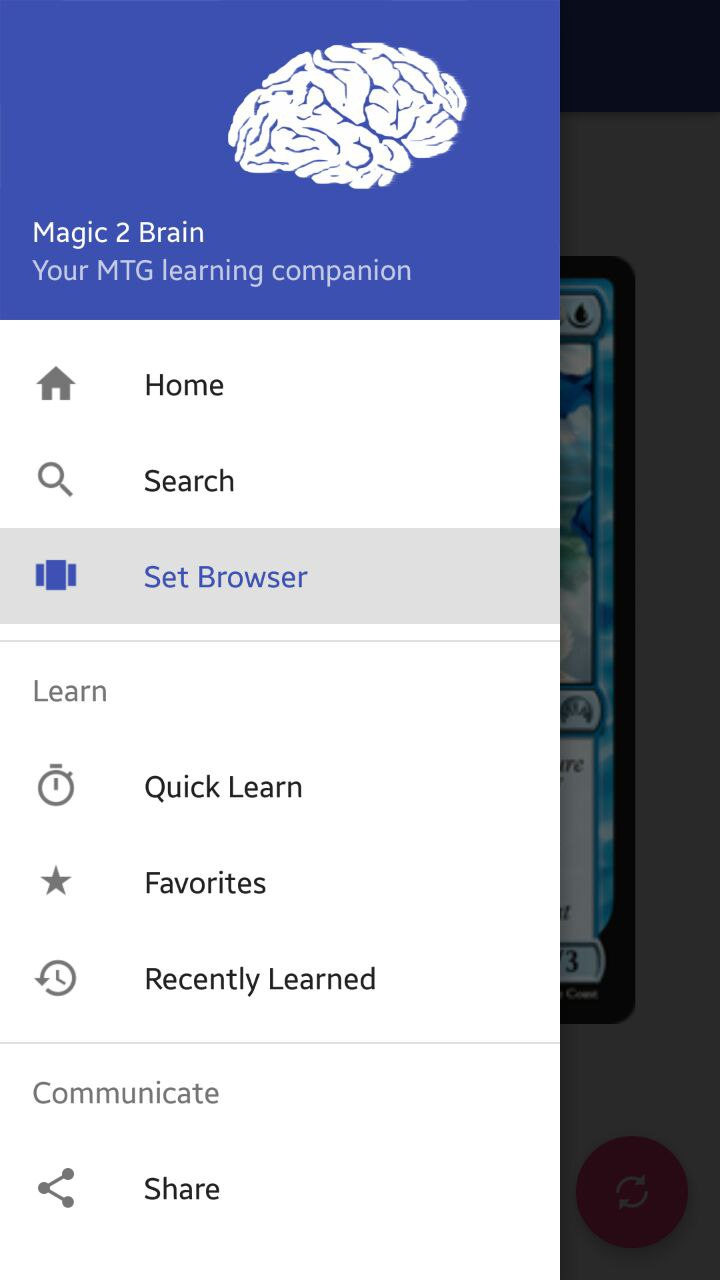
\includegraphics[width=0.3\textwidth]{sidemenu.jpg}
 \caption{Links: Der Splash-Screen, Rechts: Das Menü}
 \label{fig:splashundmenu}
\end{figure}

\subsection{Home}
Der Homescreen ist simpel aufgebaut. Ganz oben ist "`Magic2Brain"' geschrieben und direkt unter dem "`Random Card"'. Mitten auf dem Bildschirm ist eine zufällige Karte abgebildet. Mit einem Klick auf die Karte lässt sich diese vergrössern. Ganz unten rechts ist ein runder Knopf. Dieser ersetzt bei einem Klick die Karte mit einer anderen zufälligen Karte. (Abbildung \ref{fig:homemenu}).

\begin{figure}[htbp]
 \centering
    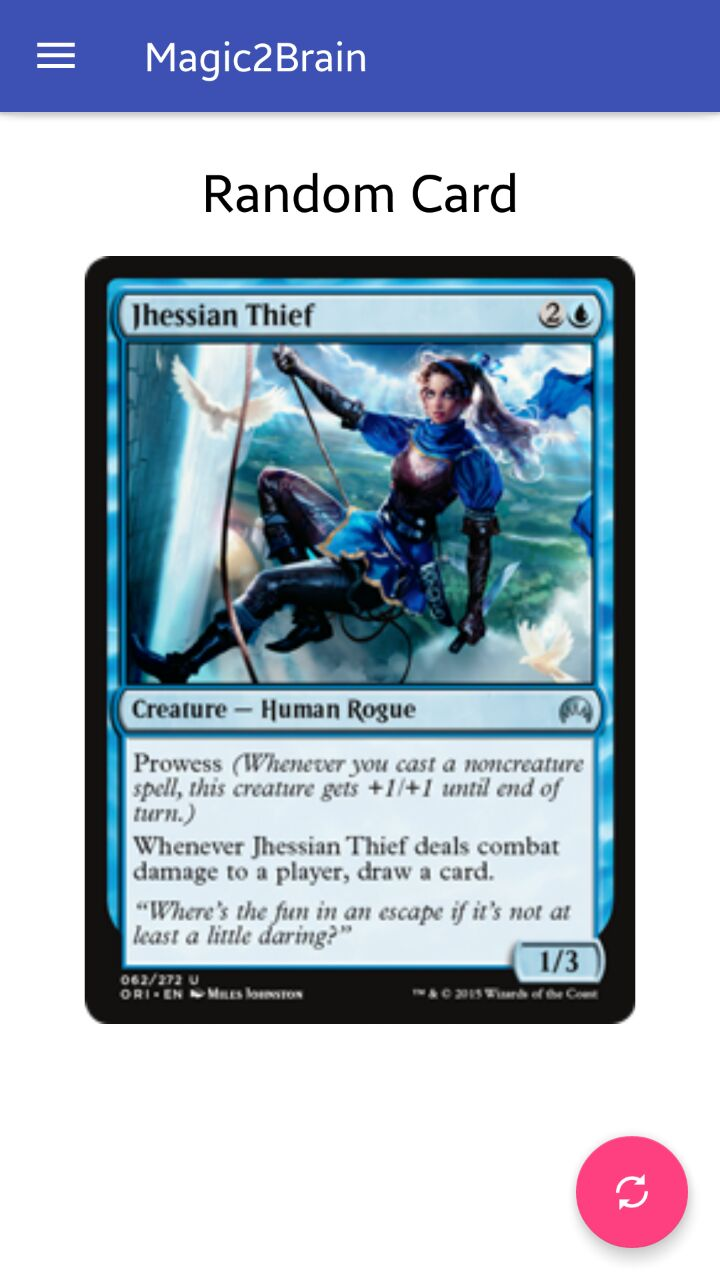
\includegraphics[width=0.3\textwidth]{home.jpg}
 \caption{Der Home-Screen \cite{Magiccard}}
 \label{fig:homemenu}
\end{figure}

\subsection{Search}
Wird auf "`Search"' gedrückt, kann ausgewählt werden, ob nach Karten oder Sets gesucht wird. Wählt man eine der beiden Optionen aus, wird man zu einer Ansicht mit einem Textfeld über einer Liste weitergeleitet. Tippt man etwas in das Textfeld ein, ändert sich die Liste und zeigt nur die Suchergebnisse an.

\subsection{Set Browser}
Der Set-Browser zeigt alle Sets in einer Liste an (Abbildung \ref{fig:setbrowser}). Drückt man auf ein Set, erscheint eine weitere Ansicht mit einer Liste. Diese Liste beinhaltet alle Karten vom ausgewählten Set. Navigiert man auf eine Karte, sieht man die Karte in einer Detailansicht. Bild, Text, Manakosten und der Name der Karte werden angezeigt (Abbildung \ref{fig:setbrowser}). Zudem hat man einen Knopf mit einem Herzen drauf. Betätigt man diesen, wird die Karte zu den Favoriten hinzugefügt.

\begin{figure}[htbp]
 \centering
    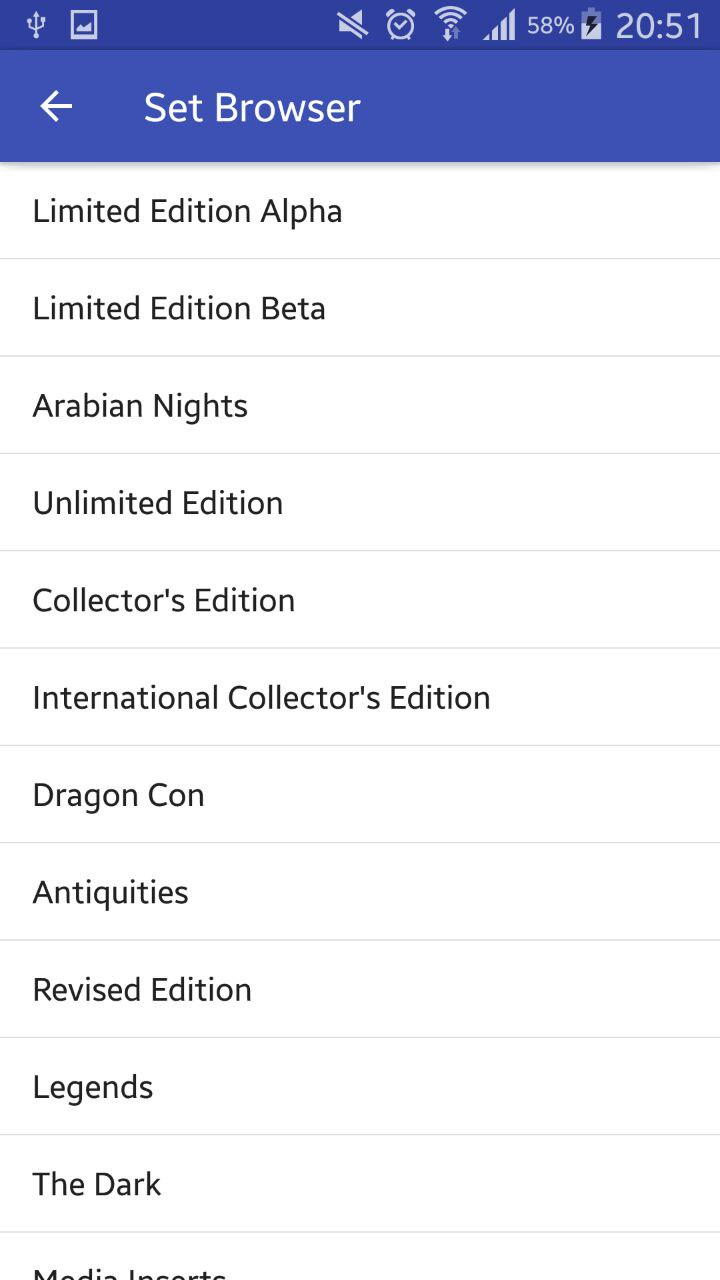
\includegraphics[width=0.3\textwidth]{setbrowser.jpg}
     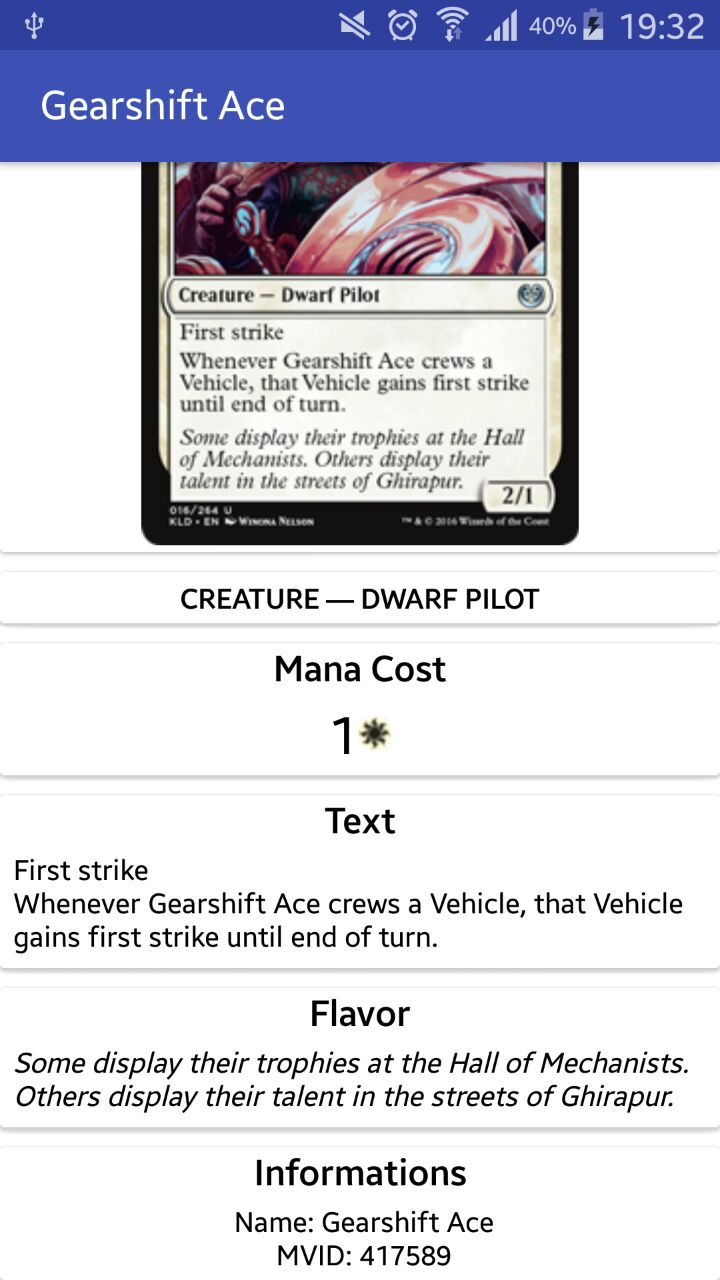
\includegraphics[width=0.3\textwidth]{cardview.jpg}
 \caption{Links: Der Set-Browser, Rechts: Die Karten-Ansicht \cite{Magiccard}}
 \label{fig:setbrowser}
\end{figure}

\subsection{Quick Learn}
"`Quick Learn"' startet eine Abfrage mit dem aktuellsten Set. In diesem Fall ist es Kaladesh. In der Mitte wird eine Karte vom Set gezeigt. Dabei ist der Text der Karte abgedeckt. Unterhalb der Karte befinden sich vier Schaltflächen mit verschiedenen Texten. Einer der Knöpfe enthält den Text der Karte. Drückt man die richtige Schaltfläche, wird kurz ein Haken auf die Karte projiziert, ansonsten ein Kreuz. Nach dieser Animation wird das Bild der Karte durch die nächste Karte im Set ersetzt. Die Schaltflächen ändern zudem ihren Text. Oben rechts befindet sich ein Menü-Sandwich. Bei dessen Betätigung sich ein Menü mit 3 Optionen öffnet: "`Query Lands"',"`Reverse query"' und "`Restart". Mit "`Query Lands"' kann man auswählen, ob die Länder auch abgefragt werden sollen. "`Reverse query" ändert den Abfragemodus. Im alternativen Modus ist der Name der Karte verdeckt. Unter der Karte befindet sich ein Textfeld, worin man den Namen der Karte eingeben soll. "`Restart" startet die ganze Abfrage neu (Abbildung \ref{fig:queryview}).

\begin{figure}[htbp]
 \centering
    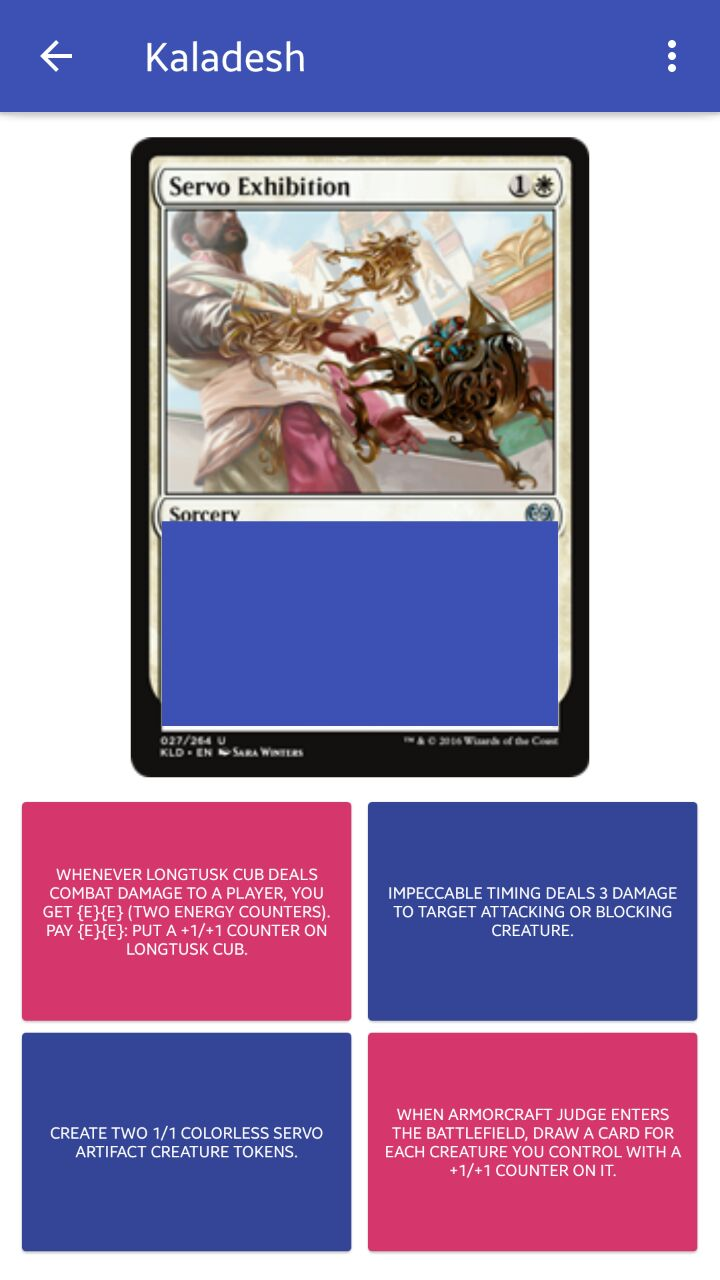
\includegraphics[width=0.3\textwidth]{query.jpg}
 \caption{Die Abfrage eines Sets \cite{Magiccard}}
 \label{fig:queryview}
\end{figure}

\subsection{Favorites}
Wechselt man auf den Reiter Favoriten, werden alle Karten, die als Favorit markiert wurden, in einer Liste angezeigt.

\subsection{Recently Learned}
"`Recently Learned"' zeigt die letzten 10 gelernten Sets in einer Liste an.

\subsection{Share}
Drückt man auf diese Schaltfläche, öffnet sich ein Menü. In diesem Menü kann man auswählen über welche App man den Link zu dieser App versenden möchte.

DISKUSSION DER ERGEBNISSE

Unsere Projektidee entstrand mit dem hinblick auf neue und bestehende Turnierspieler der Kartenspiels Magic: the Gathering (\textit{kurz: MTG}).
Jeden Monat kommt ein neues Kartenpaket heraus. Dieses wird Set genannt. Die karten in jedem Set haben andere Eigenschaften in der Angriffsstärke, der Verteidigung oder haben sogar besondere oder einzigartige Eigenschaften. Um nicht ständig diese Daten von den Karten zu lesen wollten wir eine App machen, die genau diese Daten deren Nutzern beibringt.
Ein Spiel hat nämlich auch eine zeitliche Begrenzung, die in einem Unentschieden endet. Daher ist es für beide Spieler von vorteil wenn sie schnell spielen.

Um dies zu bewerkstelligen haben wir zahlreiche APIs \textit{(\textbf{A}pplication \textbf{P}programming \textbf{I}nterface)} verglichen. Zu beachten gab es 3 grundlegende Komponenten: Bilder der Karte, Text mit Eigenschafen der Karte und Eine Möglichkeit den Fortschritt zu speichern. Die Bilder haben wir direkt von dem Kartenbrowser von Wizards of the Coast genommen. Als API für die Karteninformationen hat MTGJSON gesiegt, wobei dies keine API ist, sondern eine Downloadquelle für Karten im JSON Format. JSON ist eine schnelle und einfach zu begreifende Alternative zu XML. Somit kann die App auch offline verwendet werden. Bilder, welche einmal heruntergeladen wurden, werden bis zum deinstallieren der App oder bis zum manuellen löschen auf dem Gerät des Benutzers gespeichert. Informationen über den Fortschritt werden in den \textit{SharedPreferences} von Android gespeichert. Dies kann man sich wie ein Karteisystem vorstellen. Jede App erhält ihr eigenes Fach und kann dort Informationen ablegen.

Ursprünglich wollten wir unsere App in HTML, CSS und JavaScript schreiben, welche wir dann mit Cordova zu einer Android und IOS App kompilliert hätten.
Jedoch wurde uns durch die Natur von JavaScipt verwehrt einige essentielle Funktionen zu implementieren. Dies lag vorwiegend daran, dass JavaScript Asynchron arbeitet und man dies nicht mehr wie damals ausschalten kann. Asynchron beschreibt die Arbeitsweise von einer Programmiersprache. In diesem fall werden mehrere Funktionen gleichzeitig ausgeführt, was ein gut durch dachtes und stabiles Programm erfordert. Ausserdem müssen in einigen Fällen \textit{"Promises"} zurückgegeben werden. Das sind verweise auf einen Wert, der in der Zukunft existieren wird, aber noch nicht bekannt ist wann es so weit ist. Als Beispiel nehme man eine ladende Webseite. Niemand weiss wann sie fertig geladen ist, da das von der Verbindungsgeschwindikeit abhängt, aber der Fakt, dass sie einmal geladen sein wird ist unbestritten. Promises kann man auch nicht ohne weiters abwarten bzw. \textit{auflösen}, weil das in sehr vielen Fällen kritische auswirkungen auf die Geschwindigkeit des Programms hat. Synchrone sprachen hingegen arbeiten den Programmcode wie eine Art Stapel ab. Zeile für Zeile liest der Compiler den Code durch und wandelt ihn in Maschienensprache um. Das lässt dem Programmierer wenig Spielraum für Fehler übrig. Weil die Zeit schon relativ fortgeschritten und die App gröstenteil fertig war entschieden wir uns nur schewren Herzens dazu unser projekt aufzugeben und die App in Java zu schreiben. In Java schritten wir jedoch viel schneller voran als in JS.
 
\end{thebibliography}

\newpage

%----------------------------------------------------------------------------------------
%	Anhang
%----------------------------------------------------------------------------------------

\section{Anhang} % Major section

\subsection{MainActivity.java}
\begin{lstlisting}
package m2b.magic2brain.com;

import android.content.Intent;
import android.content.SharedPreferences;
import android.graphics.Color;
import android.os.Bundle;
import android.preference.PreferenceManager;
import android.support.design.widget.FloatingActionButton;
import android.support.design.widget.NavigationView;
import android.support.v4.view.GravityCompat;
import android.support.v4.widget.DrawerLayout;
import android.support.v7.app.ActionBarDrawerToggle;
import android.support.v7.app.AppCompatActivity;
import android.support.v7.widget.Toolbar;
import android.view.Gravity;
import android.view.MenuItem;
import android.view.View;
import android.view.Window;
import android.view.WindowManager;
import android.widget.ImageView;
import android.widget.RelativeLayout;
import android.widget.TextView;
import com.google.gson.Gson;
import com.google.gson.reflect.TypeToken;
import com.squareup.picasso.Picasso;
import java.lang.reflect.Type;
import java.util.ArrayList;
import java.util.Arrays;
import m2b.magic2brain.com.magic2brain.R;

/*
This is where our app starts. It has a menu, shows a random card and loads some needed data.
*/

public class MainActivity extends AppCompatActivity implements NavigationView.OnNavigationItemSelectedListener {

    public static Card[] cardarray; // We will store all cards in this array. This is important for the SearchActivity. It makes the whole process alot faster.
    private ImageView imgv; // We will show the random card with this ImageView

    protected void onCreate(Bundle savedInstanceState) { // This is the very first function the app will execute at the start of the app.
        if (!checkCardArray()) { // We try to load our card-list.
            saveCardArray(); // If we don't find the card-list, we have to generate it and save it.
        }
        hideStatusBar(); // Does what is says. It hides the Statusbar
        setTheme(R.style.AppTheme_NoActionBar);  // We want to hide the ActionBar too
        super.onCreate(savedInstanceState); // This does some intern stuff. We don't need to worry about that. It's just needed.
        setContentView(R.layout.activity_main); // This adds an View to our Activity. We defined at "/res/layout/activity_main.xml" how our activity should look like.
        Toolbar toolbar = (Toolbar) findViewById(R.id.toolbar); // With this we get the Toolbar of the View.
        setSupportActionBar(toolbar); // We add the Toolbar as a SupportActionBar. If we click something on the Toolbar it will call onNavigationItemSelected();

        FloatingActionButton fab = (FloatingActionButton) findViewById(R.id.fab); // We get the "new random card"-button
        fab.setOnClickListener(new View.OnClickListener() {
            public void onClick(View view) {
                setListener(setRandomCard()); // If we click the button it should generate a new random card.
            }
        });
        // The following lines generate the drawer (Sidemenu)
        DrawerLayout drawer = (DrawerLayout) findViewById(R.id.drawer_layout);
        ActionBarDrawerToggle toggle = new ActionBarDrawerToggle(
                this, drawer, toolbar, R.string.navigation_drawer_open, R.string.navigation_drawer_close);
        drawer.setDrawerListener(toggle);
        toggle.syncState();
        NavigationView navigationView = (NavigationView) findViewById(R.id.nav_view);
        navigationView.setNavigationItemSelectedListener(this);

        Favorites.init(); // Initate Favorites

        // The following code loads the Favorites from the memory
        SharedPreferences appSharedPrefs = PreferenceManager.getDefaultSharedPreferences(this);
        Gson gson = new Gson();
        String json = appSharedPrefs.getString("favobj", null);
        Type type = new TypeToken<ArrayList<Card>>() {
        }.getType();
        ArrayList<Card> favs = gson.fromJson(json, type);
        Favorites.init();
        if (favs != null) {
            Favorites.favorites_mvid = favs;
        }
        buildNewsFeed(); // This builds the frontpage
    }

    private void hideStatusBar() { // This method simply removes the Statusbar
        requestWindowFeature(Window.FEATURE_NO_TITLE); // remove the title
        getWindow().setFlags(WindowManager.LayoutParams.FLAG_FULLSCREEN, WindowManager.LayoutParams.FLAG_FULLSCREEN); // set it to fullscreen
    }

    protected void onPause() {
        super.onPause();
        // If the user leaves our app in any way, we save all his favorites.
        SharedPreferences appSharedPrefs = PreferenceManager.getDefaultSharedPreferences(this);
        SharedPreferences.Editor prefsEditor = appSharedPrefs.edit();
        Gson gson = new Gson();
        String json = gson.toJson(Favorites.favorites_mvid);
        prefsEditor.putString("favobj", json);
        prefsEditor.commit();
    }

    public void onBackPressed() { // Closes the Drawer if we press the Back-Button on the phone
        DrawerLayout drawer = (DrawerLayout) findViewById(R.id.drawer_layout);
        if (drawer.isDrawerOpen(GravityCompat.START)) {
            drawer.closeDrawer(GravityCompat.START);
        } else {
            super.onBackPressed();
        }
    }

    public boolean onNavigationItemSelected(MenuItem item) {
        // Handle navigation view item clicks here.
        int id = item.getItemId();
        if (id == R.id.nav_search) {
            // Starts the SearchActivitiy if we click on Search
            Intent intent = new Intent(this, SearchActivity.class);
            startActivity(intent);

        } else if (id == R.id.nav_favorite) {
            // Starts the FavoritesActivity if we click ond Favorites
            Intent intent = new Intent(this, FavoritesActivity.class);
            startActivity(intent);

        } else if (id == R.id.nav_browser) {
            // Starts the BrowserActivity if we click on the Cardbrowser
            Intent intent = new Intent(this, BrowserActivity.class);
            startActivity(intent);

        } else if (id == R.id.nav_quick_learn) {
            // Starts the QueryActivity and passes the newest set (Kaladesh), if we click Quick learn
            Deck d = new Deck();
            Card[] c = DeckAssetLoader.getDeck("KLD.json",this);
            d.setSet(c);
            d.setName("Kaladesh");
            d.setCode("KLD");
            Intent i = new Intent(this, QueryActivity.class);
            i.putExtra("Set", d);
            startActivity(i);

        } else if (id == R.id.nav_history) {
            // Starts the LastSeenActivity if we click recently learned
            Intent intent = new Intent(this, LastSeenActivity.class);
            startActivity(intent);

        } else if (id == R.id.nav_share) {
            // Starts an Activity, which opens all possibilities to send the link to our app.
            Intent sendIntent = new Intent();
            sendIntent.setAction(Intent.ACTION_SEND);
            sendIntent.putExtra(Intent.EXTRA_TEXT, getString(R.string.play_store_link));
            sendIntent.setType("text/plain");
            startActivity(Intent.createChooser(sendIntent, getResources().getText(R.string.send_to)));
        }

        DrawerLayout drawer = (DrawerLayout) findViewById(R.id.drawer_layout); // We get the drawer
        drawer.closeDrawer(GravityCompat.START); // Th drawer should start closed
        return true;
    }

    public void buildNewsFeed() { // This Function generates a text and a Imageview on the screen
        int scrWidth = getWindowManager().getDefaultDisplay().getWidth(); // Get the width of the screen
        int scrHeight = getWindowManager().getDefaultDisplay().getHeight(); // Get the Height of the screen
        RelativeLayout lyt = (RelativeLayout) findViewById(R.id.main_absolute); // Get the View of the XML
        RelativeLayout.LayoutParams params; // The parameters we want to add our TextView and ImageView

        TextView score = new TextView(this); // Create new Textview
        score.setTextColor(Color.BLACK);
        score.setGravity(Gravity.CENTER);
        score.setText("Random Card");
        score.setTextSize(26);
        params = new RelativeLayout.LayoutParams(scrWidth /*Width*/, (int) (0.1 * scrHeight)/*Height*/);
        params.leftMargin = 0; // X-Position
        params.topMargin = (int) (0.1 * scrHeight); // Y-Position
        lyt.addView(score, params); // add it to the View

        imgv = new ImageView(this); // Create new Imageview
        params = new RelativeLayout.LayoutParams(scrWidth /*Width*/, (int) (0.6 * scrHeight))/*Height*/;
        params.leftMargin = 0; // X-Position
        params.topMargin = (int) (0.2 * scrHeight); // Y-Position
        lyt.addView(imgv, params); // add it to the View
        setListener(setRandomCard()); // Opens a random card
    }

    public void setListener(int MultiID2) { // This function sets an listener to the image, so if we click it, it shows a big image of the card.
        final int MultiID = MultiID2;
        imgv.setOnClickListener(new View.OnClickListener() {
            public void onClick(View view) {
                Intent intent = new Intent(MainActivity.this, CardImageDisplayActivity.class);
                intent.putExtra("pic", MultiID);
                startActivity(intent);
            }
        });
    }

    public int setRandomCard() { // This gets a random card from the card-array and loads the image into the ImageView
        int MultiID = 1;
        Card c = cardarray[(int) (Math.random() * cardarray.length)];
        if (c != null) {
            MultiID = c.getMultiverseid();
        }
        Picasso.with(this)
                .load(getString(R.string.image_link_1) + MultiID +  getString(R.string.image_link_2)) // This tries to load an image from a link.
                .placeholder(R.drawable.loading_image) // We want to show a image while its loading. We load our image from the "/res/drawable" folder
                .error(R.drawable.image_not_found)  // If it fails to load image we show an error-image.
                .into(imgv);  // This places the image into our ImageView.
        return MultiID;
    }

    public boolean checkCardArray() { // This method checks if there is a saved version of our card array. If that's the case it tries to load it into the card-array.
        SharedPreferences sharedPrefs = PreferenceManager.getDefaultSharedPreferences(this);
        Gson gson = new Gson();
        String json = sharedPrefs.getString("cardArray", null);
        Type type = new TypeToken<Card[]>() {
        }.getType();
        Card[] aL = gson.fromJson(json, type);
        if (aL == null) {return false;}
        cardarray = aL;
        return true;
    }

    public void saveCardArray() { // This function saves the card-array into the memory.
        Card[] c = buildCardArray();
        SharedPreferences sharedPrefs = PreferenceManager.getDefaultSharedPreferences(this);
        SharedPreferences.Editor editor = sharedPrefs.edit();
        Gson gson = new Gson();
        String json = gson.toJson(c);
        editor.putString("cardArray", json);
        editor.commit();
        cardarray = c;
    }

    private Card[] buildCardArray() { // This method generates the card-array by opening all sets and loading the cards from it into out array.
        ArrayList<Card> list = new ArrayList<>();
        Deck[] deckarray = DeckAssetLoader.getDeckList(this);
        for (int i = 0; i < deckarray.length; i++) {
            //load current deck and append it to list
            Card[] c = DeckAssetLoader.getDeck(deckarray[i].getCode() + ".json", this);
            if (c[0].getName().equals("error")) {
                System.err.println("error ocurred at " + deckarray[i].getCode() + ", please update your database");
            } else {
                list.addAll(Arrays.asList(c));
            }
        }
        return list.toArray(new Card[list.size()]);
    }
}
\end{lstlisting}
\newpage
\subsection{SearchActivity.java}
\begin{lstlisting}
package m2b.magic2brain.com;

import android.content.Context;
import android.content.Intent;
import android.os.Bundle;
import android.support.v7.app.AppCompatActivity;
import android.view.MenuItem;
import android.view.View;
import android.view.View.OnClickListener;
import android.widget.Button;
import m2b.magic2brain.com.magic2brain.R;

/*
This Activity asks the user if he wants to search for cards or set and opens a SearchHandlerActivity if the answer.
*/

public class SearchActivity extends AppCompatActivity {

    protected void onCreate(Bundle savedInstanceState) {
        overridePendingTransition(R.anim.slide_in_left, R.anim.slide_out_left); // This adds an fancy slide animation, when this activity starts.
        super.onCreate(savedInstanceState); // This does some intern stuff. We don't need to worry about that. It's just needed.
        setContentView(R.layout.activity_search); // This adds an View to our Activity. We defined at "/res/layout/activity_search.xml" how our activity should look like.
        getSupportActionBar().setDisplayHomeAsUpEnabled(true); // With this line we add an "back"-Button to the Toolbar. If we press it it calls onOptionsItemSelected();
        final Context context = this; // This doesn't actually do anything, but it's needed if we want to refer to "this" from an inner class.
        setTitle(getString(R.string.SearchActivity_title)); // We set a title to our View. We defined the title in "/res/values/strings.xml". We just load it from there.
        Button cards = (Button) findViewById(R.id.c_search_cards); // We get the cards-button
        Button decks = (Button) findViewById(R.id.c_search_decks); // We get the sets-button

        cards.setOnClickListener(new OnClickListener() {
            public void onClick(View view) {
                // If the user presses the cards-button, we start SearchHandlerActivity and pass to it, that the user pressed "cards"
                Intent intent = new Intent(context, SearchHandlerActivity.class);
                intent.putExtra("cardsearch", true);
                startActivity(intent);
            }
        });

        decks.setOnClickListener(new OnClickListener() {
            public void onClick(View view) {
                // If the user presses the sets-button, we start SearchHandlerActivity and pass to it, that the user pressed "sets"
                Intent intent = new Intent(context, SearchHandlerActivity.class);
                intent.putExtra("cardsearch", false);
                startActivity(intent);
            }
        });
    }

    public boolean onOptionsItemSelected(MenuItem item) {
        switch (item.getItemId()) {
            // Respond to the action bar's Up/Home button
            case android.R.id.home:
                onBackPressed();
        }
        return true;
    }

    public void onBackPressed() {
        finish(); // This closes our Activity
        overridePendingTransition(R.anim.slide_in_right, R.anim.slide_out_right); // We want to close it with an fancy animation.
    }
}

\end{lstlisting}
\newpage
\subsection{SearchHandlerActivity.java}
\begin{lstlisting}
package m2b.magic2brain.com;

import android.content.Context;
import android.content.Intent;
import android.os.Bundle;
import android.support.v7.app.AppCompatActivity;
import android.text.Editable;
import android.text.TextWatcher;
import android.view.MenuItem;
import android.view.View;
import android.widget.AdapterView;
import android.widget.ArrayAdapter;
import android.widget.EditText;
import android.widget.ListView;
import m2b.magic2brain.com.magic2brain.R;

/*
This Activity is the one that actually searches for cards/sets.
*/

public class SearchHandlerActivity extends AppCompatActivity {
    Card[] cardarray; // This is the array, where all cards are stored

    protected void onCreate(Bundle savedInstanceState) {
        overridePendingTransition(R.anim.slide_in_left, R.anim.slide_out_left); // This adds an fancy slide animation, when this activity starts.
        super.onCreate(savedInstanceState);  // This does some intern stuff. We don't need to worry about that. It's just needed.
        setContentView(R.layout.activity_search_handler); // This adds an View to our Activity. We defined at "/res/layout/activity_search_handler.xml" how our activity should look like.
        getSupportActionBar().setDisplayHomeAsUpEnabled(true); // With this line we add an "back"-Button to the Toolbar. If we press it it calls onOptionsItemSelected();

        final Context context = this; // This doesn't actually do anything, but it's needed if we want to refer to "this" from an inner class.
        Intent inte = getIntent();  // We want to access any data that is passed.
        final Boolean cardsearch = inte.getBooleanExtra("cardsearch", true); // We look if the user wants to search for a card or set

        final EditText search_field = (EditText) findViewById(R.id.search_text); // We get the search-field
        if (cardsearch) {
            search_field.setHint(R.string.SearchHandler_hint_1); // if he wants to search a card, we set the hint to "Cardname"
        } else {
            search_field.setHint(R.string.SearchHandler_hint_2); // if he wants to search a set, we set the hint to "Setname"
        }
        final ListView searchresultsview = (ListView) findViewById(R.id.search_lv); // We get the ListView so we can show the results

        String[] names = new String[1]; // We only need the names so we create a names-array
        names[0] = getString(R.string.error); // This is to ensure that the array isn't empty
        Deck[] deckarray = DeckAssetLoader.getDeckList(this); // We get all decks


        if (cardsearch) {
            cardarray = MainActivity.cardarray; // We load our card-array
            names = new String[cardarray.length];

            for (int i = 0; i < cardarray.length; i++) {
                names[i] = cardarray[i].getName(); // And add all names to the string-array
            }
        } else {
            names = new String[deckarray.length]; // The same like cards but with sets

            for (int i = 0; i < deckarray.length; i++) {
                names[i] = deckarray[i].getName();  // The same like cards but with sets
            }
        }

        //finalizing variables for further use
        final Deck[] cdeckarray = deckarray;
        final Card[] ccardarray = cardarray;


        final ArrayAdapter adapter = new ArrayAdapter(context, android.R.layout.simple_list_item_1, names); // We turn the string-array into a list
        search_field.addTextChangedListener(new TextWatcher() { // and add a listener, so it updates when we write something
            public void beforeTextChanged(CharSequence charSequence, int i, int i1, int i2) {}
            public void onTextChanged(CharSequence charSequence, int i, int i1, int i2) {}
            public void afterTextChanged(Editable editable) {
                adapter.getFilter().filter(editable.toString().toLowerCase());
            }
        });

        searchresultsview.setAdapter(adapter); // We show the list
        searchresultsview.setOnItemClickListener(new AdapterView.OnItemClickListener() {
            public void onItemClick(AdapterView<?> parent, View view, int position, long id) {
                if (cardsearch) {
                    // If it's a card-search, we open CardBrowserActivity with the clicked card.
                    String cardname = adapter.getItem(position).toString();
                    Intent intent = new Intent(context, CardBrowserActivity.class);
                    intent.putExtra("currentCard", searchforcard(cardname, ccardarray));
                    startActivity(intent);
                } else {
                    // If it's a set-search, we open DeckDisplayActivity with the clicked Set
                    String deckname = adapter.getItem(position).toString();
                    Intent intent = new Intent(context, DeckDisplayActivity.class);
                    intent.putExtra("code", searchfordeck(deckname, cdeckarray));
                    intent.putExtra("name", deckname);
                    startActivity(intent);
                }
            }
        });

    }

    private Card searchforcard(String name, Card[] cardarray) { // This function searchs for a card and returns it
        Card rc = new Card();

        for (int i = 0; i < cardarray.length; i++) {
            if (cardarray[i].getName().equals(name)) {
                rc = cardarray[i];
                break;
            }
        }
        return rc;
    }

    private String searchfordeck(String name, Deck[] darray) { // This function searchs for a set and returns it
        String code = getString(R.string.error);

        for (int i = 0; i < darray.length; i++) {
            String dname = darray[i].getName();

            if (dname.equals(name)) {
                code = darray[i].getCode();
                break;
            }
        }

        return code;
    }

    public boolean onOptionsItemSelected(MenuItem item) {
        int id = item.getItemId();
        switch (id) {
            // Respond to the action bar's Up/Home button
            case android.R.id.home:
                onBackPressed();
        }
        return true;
    }

    public void onBackPressed() {
        finish(); // This closes our Activity
        overridePendingTransition(R.anim.slide_in_right, R.anim.slide_out_right); // We want to close it with an fancy animation.
    }
}

\end{lstlisting}
\newpage
\subsection{BrowserActivity.java}
\begin{lstlisting}
package m2b.magic2brain.com;

import android.content.Context;
import android.content.Intent;
import android.os.Bundle;
import android.support.v7.app.AppCompatActivity;
import android.support.v7.widget.Toolbar;
import android.view.MenuItem;
import android.view.View;
import android.widget.AdapterView;
import android.widget.AdapterView.OnItemClickListener;
import android.widget.ArrayAdapter;
import android.widget.ListView;
import m2b.magic2brain.com.magic2brain.R;

/*
This Activity should show a List with all sets and open DeckDisplayActivity with the selected set on a click.
*/

public class BrowserActivity extends AppCompatActivity {

    protected void onCreate(Bundle savedInstanceState) {
        overridePendingTransition(R.anim.slide_in_left, R.anim.slide_out_left); // This adds an fancy slide animation, when this activity starts.
        super.onCreate(savedInstanceState); // This does some intern stuff. We don't need to worry about that. It's just needed.
        setContentView(R.layout.activity_browser); // This adds an View to our Activity. We defined at "/res/layout/activity_browser.xml" how our activity should look like.
        Toolbar toolbar = (Toolbar) findViewById(R.id.toolbar); // With this we get the Toolbar of the View.
        setSupportActionBar(toolbar); // We add the Toolbar as a SupportActionBar. This is needed for the next line.
        getSupportActionBar().setDisplayHomeAsUpEnabled(true); // With this line we add an "back"-Button to the Toolbar. If we press it it calls onOptionsItemSelected();
        setTitle(getString(R.string.BrowserActivity_title)); // We set a title to our View. We defined the title in "/res/values/strings.xml". We just load it from there.
        final Context currentContext = this; // This doesn't actually do anything, but it's needed if we want to refer to "this" from an inner class.

        Deck d[] = DeckAssetLoader.getDeckList(this); // We load all Sets with our own function into an Deck-Array.
        String[] it = new String[d.length]; // We just need the names of the sets. So we create an String-Array for the names.
        for (int i = 0; i < d.length; i++) {
            it[i] = d[i].getName();  // This for-loop adds the names from every Deck from the Deck-Array to the String-Array.
        }

        final String[] listItems = it; // We need to finalize the String-Array for the ArrayAdapter.
        final Deck[] finalD = d; // We need to finalize the Deck-Array, because we want to access it from an inner class.
        final ArrayAdapter adapter = new ArrayAdapter(this, android.R.layout.simple_list_item_1, listItems); // This is just a helper-class. It transforms our String-Array into an clickable List.
        ListView lv = (ListView) findViewById(R.id.deckbrowser_list); // We want to add our list to the ListView. So we get the ListView from the View
        lv.setAdapter(adapter); // We add our list into it.


        lv.setOnItemClickListener(new OnItemClickListener() { // This performs an action when we click on an item from the list.
            public void onItemClick(AdapterView<?> parent, View view, int position, long id) {
                // The following code starts DeckDisplayActivity and passes the Deck-Code and the Deck-Name of the item we clicked.
                Intent intent = new Intent(currentContext, DeckDisplayActivity.class);
                intent.putExtra("code", finalD[position].getCode());
                intent.putExtra("name", finalD[position].getName());
                startActivity(intent);
            }
        });
    }

    public boolean onOptionsItemSelected(MenuItem item) {
        switch (item.getItemId()) {
            // Respond to the action bar's Up/Home button
            case android.R.id.home:
                onBackPressed();
        }
        return true;
    }

    public void onBackPressed() {
        finish(); // This closes our Activity
        overridePendingTransition(R.anim.slide_in_right, R.anim.slide_out_right); // We want to close it with an fancy animation.
    }

}
\end{lstlisting}
\newpage
\subsection{DeckDisplayActivity.java}
\begin{lstlisting}
package m2b.magic2brain.com;

import android.content.Context;
import android.content.DialogInterface;
import android.content.Intent;
import android.os.Bundle;
import android.support.design.widget.FloatingActionButton;
import android.support.v7.app.AlertDialog;
import android.support.v7.app.AppCompatActivity;
import android.view.MenuItem;
import android.view.View;
import android.widget.AdapterView;
import android.widget.AdapterView.OnItemClickListener;
import android.widget.ArrayAdapter;
import android.widget.ListView;
import java.util.ArrayList;
import java.util.Arrays;
import java.util.List;
import m2b.magic2brain.com.magic2brain.R;

/*
This class shows all cards of a deck in a list
 */
public class DeckDisplayActivity extends AppCompatActivity {

    protected void onCreate(Bundle savedInstanceState) {
        overridePendingTransition(R.anim.slide_in_left, R.anim.slide_out_left); // This adds an fancy slide animation, when this activity starts.
        super.onCreate(savedInstanceState); // This does some intern stuff. We don't need to worry about that. It's just needed.
        setContentView(R.layout.activity_deck_display); // This adds an View to our Activity. We defined at "/res/layout/activity_deck_display.xml" how our activity should look like.
        getSupportActionBar().setDisplayHomeAsUpEnabled(true); // With this line we add an "back"-Button to the Toolbar. If we press it it calls onOptionsItemSelected();

        final Context currentContext = this; // This doesn't actually do anything, but it's needed if we want to refer to "this" from an inner class.
        Intent intent = getIntent(); // We want to access any data that is passed.
        final String deckcode = intent.getStringExtra("code"); // we get the deck-code
        final String name = intent.getStringExtra("name"); // we get the deck-name

        setTitle(name); // We set the title of the activity to the name of the deck
        Card c[] = DeckAssetLoader.getDeck(deckcode + ".json", this); // This gets all the cards from the deck
        final Card[] cCopy = c; // and adds it to an Array

        FloatingActionButton fam = (FloatingActionButton) findViewById(R.id.fab_setlearn); // This gets the "Learn"-Button
        fam.setOnClickListener(new View.OnClickListener() { // and adds a listener to it
            public void onClick(View view) {
                // The following code starts the QueryActivity and passes the deck
                Intent intent = new Intent(currentContext, QueryActivity.class);
                Deck d = new Deck();
                List<Card> clist = Arrays.asList(cCopy);
                d.setCode(deckcode);
                d.setName(name);
                d.setSet(new ArrayList<Card>(clist));
                intent.putExtra("Set", d);
                startActivity(intent);
            }
        });

        ListView lv = (ListView) findViewById(R.id.deckdisplay); // We get the Listview

        if (c[0] == null) { // If there are no cards in the deck, we show an error message
            AlertDialog.Builder dlgAlert = new AlertDialog.Builder(this);
            dlgAlert.setMessage("Sadly, this Deck was not Found");
            dlgAlert.setTitle("Error");
            dlgAlert.setPositiveButton("I understand, bill me your server costs",
                    new DialogInterface.OnClickListener() {
                        public void onClick(DialogInterface dialog, int which) {
                            //dismiss the dialog
                            onBackPressed();
                        }
                    });
            dlgAlert.setCancelable(true);
            dlgAlert.create().show();

            lv.setVisibility(View.GONE);
            fam.setVisibility(View.GONE);
        } else { // If there are some cards in the deck, we generate a card-list like we did in various other Activities
            final String[] listItems = RUtils.getListified(c);
            final ArrayAdapter adapter = new ArrayAdapter(this, android.R.layout.simple_list_item_1, listItems);
            lv.setAdapter(adapter);

            final Card[] finalC = c;

            lv.setOnItemClickListener(new OnItemClickListener() {
                public void onItemClick(AdapterView<?> parent, View view, int position, long id) {
                    Intent intent = new Intent(currentContext, CardBrowserActivity.class);
                    intent.putExtra("currentCard", finalC[position]);
                    startActivity(intent);
                }
            });
        }
    }

    public boolean onOptionsItemSelected(MenuItem item) {
        int id = item.getItemId();
        switch (id) {
            // Respond to the action bar's Up/Home button
            case android.R.id.home:
            onBackPressed();
        }
        return true;
    }

    public void onBackPressed() {
        finish(); // This closes our Activity
        overridePendingTransition(R.anim.slide_in_right, R.anim.slide_out_right); // We want to close it with an fancy animation.
    }
}
\end{lstlisting}
\newpage
\subsection{CardBrowserActivity.java}
\begin{lstlisting}
package m2b.magic2brain.com;

import android.content.Context;
import android.content.Intent;
import android.graphics.Color;
import android.os.Bundle;
import android.support.design.widget.FloatingActionButton;
import android.support.design.widget.Snackbar;
import android.support.v7.app.AppCompatActivity;
import android.support.v7.widget.Toolbar;
import android.util.TypedValue;
import android.view.Gravity;
import android.view.View;
import android.widget.ImageView;
import android.widget.LinearLayout;
import android.widget.TextView;
import com.squareup.picasso.Picasso;
import java.util.ArrayList;
import java.util.Arrays;
import m2b.magic2brain.com.magic2brain.R;

/*
This activity should show one card with all informations
*/
public class CardBrowserActivity extends AppCompatActivity {

    ImageView cImage; // We will store our ImageView in a global variable, because we want to acces it from various methods.

    protected void onCreate(final Bundle savedInstanceState) {
        overridePendingTransition(R.anim.slide_in_left, R.anim.slide_out_left); // This adds an fancy slide animation, when this activity starts.
        final Context context = this; // This doesn't actually do anything, but it's needed if we want to refer to "this" from an inner class.
        super.onCreate(savedInstanceState); // This does some intern stuff. We don't need to worry about that. It's just needed.

        Intent mIntent = getIntent(); // We want to access any data that is passed.
        final Card card = (Card) mIntent.getSerializableExtra("currentCard"); // We load the card-object from the Intent

        setContentView(R.layout.activity_card_browser);  // This adds an View to our Activity. We defined at "/res/layout/activity_card_browser.xml" how our activity should look like.
        Toolbar toolbar = (Toolbar) findViewById(R.id.toolbar); // With this we get the Toolbar of the View.
        toolbar.setTitle(card.getName()); // We set a title to our View. The title should be the name of the card.
        setSupportActionBar(toolbar); // We add the Toolbar as a SupportActionBar.

        cImage = (ImageView) findViewById(R.id.cbaImage); // We load our ImageView from the View
        cImage.setPadding(0, 10, 0, 10); // We add a padding to it.

        // The next couple lines builds a GUI with the informations from the card. We access all Views from our View.
        TextView tv = (TextView) findViewById(R.id.cbaInfo);
        String info = "";
        info += " Name: " + card.getName();
        info += "\n MVID: " + card.getMultiverseid();
        tv.setText(info);
        tv.setTextColor(Color.BLACK);
        tv.setPadding(0, 10, 0, 10);

        TextView text = (TextView) findViewById(R.id.cbaText);
        text.setText(card.getText());
        text.setTextColor(Color.BLACK);
        text.setPadding(20, 10, 10, 20);

        TextView flavor = (TextView) findViewById(R.id.cbaFlavor);
        flavor.setText(card.getFlavor());
        flavor.setTextColor(Color.BLACK);
        flavor.setPadding(20, 10, 10, 20);

        TextView type = (TextView) findViewById(R.id.cbaType);
        type.setText(card.getType());
        type.setTextColor(Color.BLACK);
        type.setPadding(0, 10, 0, 10);

        LinearLayout ll = (LinearLayout) findViewById(R.id.cba_mcost_layout);
        setManaCost(card.getManaCost(), ll);
        ll.setGravity(Gravity.CENTER);
        ll.setPadding(0, 10, 0, 10);

        final int mvid = card.getMultiverseid(); // This gets the MultiverseID from the card
        showPic(mvid); // and loads the picture of the card.

        cImage.setOnClickListener(new View.OnClickListener() {  // This performs an action if we click the image
            public void onClick(View view) {
                // The following code starts the CardImageDisplayActivity and passes the MultiverseID of the Card.
                Intent intent = new Intent(context, CardImageDisplayActivity.class);
                intent.putExtra("pic", mvid);
                startActivity(intent);
            }
        });

        final FloatingActionButton fab = (FloatingActionButton) findViewById(R.id.fab); // This gets our "add to favorites"-button from the view
        // We check if its already added to favorites. If so we mark it as already added.
        if (!checkCard(card.getName())) {
            fab.setImageResource(R.drawable.ic_favorite_border);
        } else {
            fab.setImageResource(R.drawable.ic_favorite);
        }

        fab.setOnClickListener(new View.OnClickListener() { // This performs an action if we click the "add to favorites"-Button
            // The following code toggles the Button, so it shows that the card was added or not, gives a notification and add the card to the favorites-list (which will be saved).
            public void onClick(View view) {
                if (checkCard(card.getName())) {
                    removeCard(card.getName());
                    fab.setImageResource(R.drawable.ic_favorite_border);
                    Snackbar.make(view, R.string.remove_fav, Snackbar.LENGTH_LONG)
                            .setAction("Action", null).show();
                } else {
                    Favorites.favorites_mvid.add(card);
                    fab.setImageResource(R.drawable.ic_favorite);
                    Snackbar.make(view, R.string.add_fav, Snackbar.LENGTH_LONG)
                            .setAction("Action", null).show();
                }
            }
        });
    }

    private boolean checkCard(String name) { // This function checks if the card was added to the favorites
        for (Card c : Favorites.favorites_mvid) {
            if (c.getName().contains(name)) {
                return true;
            }
        }
        return false;
    }

    private void removeCard(String name) { // This function removes the card from the favorites-list
        ArrayList<Card> cards = new ArrayList<>();
        for (Card c : Favorites.favorites_mvid) {
            if (c.getName().contains(name)) {
                cards.add(c);
            }
        }
        for (Card c : cards) {
            Favorites.favorites_mvid.remove(c);
        }
    }

    private void setManaCost(String manatext, LinearLayout layout) { // This function adds the mana-cost to the View by loading the images.
        manatext = manatext.replaceAll("\\{", "");
        manatext = manatext.replaceAll("\\}", "");
        String[] items = manatext.split("");
        items = Arrays.copyOfRange(items, 1, items.length);

        for (int i = 0; i < items.length; i++) {
            if (RUtils.isInteger(items[i])) {
                TextView tv = new TextView(this);
                tv.setText(items[i]);
                tv.setTextSize(TypedValue.COMPLEX_UNIT_PX, 80);
                tv.setTextColor(Color.BLACK);
                layout.addView(tv);
            } else {
                ImageView imgv = new ImageView(this);
                int resid = 0;
                if (items[i].equals("B")) {
                    resid = R.drawable.b;
                } else if (items[i].equals("C")) {
                    resid = R.drawable.c;
                } else if (items[i].equals("G")) {
                    resid = R.drawable.g;
                } else if (items[i].equals("R")) {
                    resid = R.drawable.r;
                } else if (items[i].equals("U")) {
                    resid = R.drawable.u;
                } else if (items[i].equals("W")) {
                    resid = R.drawable.w;
                } else {
                    resid = R.drawable.ic_action_cancel;
                }
                imgv.setBackgroundResource(resid);
                layout.addView(imgv);
                android.view.ViewGroup.LayoutParams layoutParams = imgv.getLayoutParams();
                layoutParams.width = 60;
                layoutParams.height = 60;
                imgv.setLayoutParams(layoutParams);
            }
        }
    }

    private void showPic(int MultiID) { // This method loads an cardimage into cImage with a given MultiverseID.
        Picasso.with(this)
                .load(getString(R.string.image_link_1) + MultiID + getString(R.string.image_link_2)) // This tries to load an image from a link.
                .placeholder(R.drawable.loading_image) // We want to show a image while its loading. We load our image from the "/res/drawable" folder
                .error(R.drawable.image_not_found) // If it fails to load image we show an error-image.
                .into(cImage); // This places the image into our ImageView.
    }

    public void onBackPressed() {
        finish(); // This closes our Activity
        overridePendingTransition(R.anim.slide_in_right, R.anim.slide_out_right); // We want to close it with an fancy animation.
    }
}
\end{lstlisting}
\newpage
\subsection{CardImageDisplayActivity.java}
\begin{lstlisting}
package m2b.magic2brain.com;

import android.content.Intent;
import android.os.Bundle;
import android.os.Handler;
import android.support.v7.app.ActionBar;
import android.support.v7.app.AppCompatActivity;
import android.view.View;
import android.widget.ImageView;
import com.squareup.picasso.Picasso;
import m2b.magic2brain.com.magic2brain.R;

/*
This Activity should show a big image of a card
 */

public class CardImageDisplayActivity extends AppCompatActivity {
    private final Handler mHideHandler = new Handler();
    private View mContentView;
    private final Runnable mHidePart2Runnable = new Runnable() {
        public void run() {
            // Delayed removal of status and navigation bar
            // Note that some of these constants are new as of API 16 (Jelly Bean)
            // and API 19 (KitKat). It is safe to use them, as they are inlined
            // at compile-time and do nothing on earlier devices.
            mContentView.setSystemUiVisibility(View.SYSTEM_UI_FLAG_LOW_PROFILE
                    | View.SYSTEM_UI_FLAG_FULLSCREEN
                    | View.SYSTEM_UI_FLAG_LAYOUT_STABLE
                    | View.SYSTEM_UI_FLAG_IMMERSIVE_STICKY
                    | View.SYSTEM_UI_FLAG_LAYOUT_HIDE_NAVIGATION
                    | View.SYSTEM_UI_FLAG_HIDE_NAVIGATION);
        }
    };
    private View mControlsView;
    private final Runnable mShowPart2Runnable = new Runnable() {
        @Override
        public void run() {
            // Delayed display of UI elements
            ActionBar actionBar = getSupportActionBar();
            if (actionBar != null) {
                actionBar.show();
            }
            mControlsView.setVisibility(View.VISIBLE);
        }
    };

    protected void onCreate(Bundle savedInstanceState) {
        super.onCreate(savedInstanceState);
        setContentView(R.layout.activity_card_image_display);

        mControlsView = findViewById(R.id.fullscreen_content_controls);
        mContentView = findViewById(R.id.fullscreen_content);
        Intent mIntent = getIntent();

        // Set up the user interaction to manually show or hide the system UI.
        mContentView.setOnClickListener(new View.OnClickListener() {
            public void onClick(View view) {
                finish();
            }
        });

        // Upon interacting with UI controls, delay any scheduled hide()
        // operations to prevent the jarring behavior of controls going away
        // while interacting with the UI.
        hide();

        int mvid = mIntent.getIntExtra("pic", 0);
        showPic(mvid);
    }

    private void showPic(int MultiID) {
        ImageView cImage = (ImageView) findViewById(R.id.cida_imgview);
        Picasso.with(this)
                .load(getString(R.string.image_link_1) + MultiID + getString(R.string.image_link_2))
                .placeholder(R.drawable.loading_image)
                .error(R.drawable.image_not_found)
                .into(cImage);
    }

    private void hide() {
        // Hide UI first
        ActionBar actionBar = getSupportActionBar();
        if (actionBar != null) {
            actionBar.hide();
        }
        mControlsView.setVisibility(View.GONE);
        // Schedule a runnable to remove the status and navigation bar after a delay
        mHideHandler.removeCallbacks(mShowPart2Runnable);
        mHidePart2Runnable.run();
    }
}
\end{lstlisting}
\newpage
\subsection{QueryActivity.java}
\begin{lstlisting}
package m2b.magic2brain.com;

import android.content.Intent;
import android.content.SharedPreferences;
import android.graphics.Color;
import android.graphics.PorterDuff;
import android.os.Bundle;
import android.os.Handler;
import android.preference.PreferenceManager;
import android.support.v7.app.AppCompatActivity;
import android.support.v7.widget.Toolbar;
import android.view.Gravity;
import android.view.KeyEvent;
import android.view.Menu;
import android.view.MenuItem;
import android.view.View;
import android.view.WindowManager;
import android.view.animation.AccelerateInterpolator;
import android.view.animation.Animation;
import android.view.animation.AnimationUtils;
import android.view.animation.DecelerateInterpolator;
import android.widget.Button;
import android.widget.EditText;
import android.widget.ImageView;
import android.widget.RelativeLayout;
import android.widget.TextView;
import com.google.gson.Gson;
import com.google.gson.reflect.TypeToken;
import com.squareup.picasso.Picasso;
import java.lang.reflect.Type;
import java.util.ArrayList;
import java.util.Collections;
import java.util.Random;
import m2b.magic2brain.com.magic2brain.R;

public class QueryActivity extends AppCompatActivity {
    private ImageView imgv; // The image of the card gets stored here
    private ImageView imgCorr; // Is over the image. It's to indicate if the answer was correct or not
    private Toolbar hiding; // This is a bar that hides a certain area
    private ArrayList<Card> set; //This Arraylist holds all Cards that need to query. It won't be edited (after loading it)
    private ArrayList<Card> wrongGuessed;
    private int indexCard; // Actually not needed (because we remove cards from WrongGuessed) but may be useful in later edits
    private boolean firstGuess; //This is to check if he guessed it at first try. If so we remove the card from the Arraylist. Else it stays there.
    private String deckName; //Name of the deck. Only for saving/loading purpose
    private TextView score; //this will show the user the current progress
    private boolean queryLand = true; // should we really query lands?
    private boolean skipped = false; // this is to store if the user has skipped or not
    private ArrayList<String> recentlyLearned; // this is to save the deckname if a new set is learned
    private ArrayList<String> recentlyLearnedNames; // the name of the sets
    private int Mode; // the query mode
    private ArrayList<Button> choices; // We store the buttons here

    protected void onCreate(Bundle savedInstanceState) {
        // Standard stuff
        overridePendingTransition(R.anim.slide_in_left, R.anim.slide_out_left); // This adds an fancy slide animation, when this activity starts.
        super.onCreate(savedInstanceState); // This does some intern stuff. We don't need to worry about that. It's just needed.
        setContentView(R.layout.activity_query); // This adds an View to our Activity. We defined at "/res/layout/activity_query.xml" how our activity should look like.
        // Hide the status bar.
        this.getWindow().setFlags(WindowManager.LayoutParams.FLAG_FULLSCREEN, WindowManager.LayoutParams.FLAG_FULLSCREEN);
        // Get some informations
        Intent i = getIntent();
        Deck qur = (Deck) i.getSerializableExtra("Set");
        deckName = qur.getName(); // Get the name of the Deck
        String code = qur.getCode(); // Get the Deck-Code
        if (deckName == null) {
            deckName = "DEFAULT"; // If deckname isn't defined, we set it to "DEFAULT"
        }
        setTitle(deckName); // we set the title to the deckname
        //Add set to recent learned
        if (!loadRecent()) {
            recentlyLearned = new ArrayList<>();
            recentlyLearnedNames = new ArrayList<>();
        }
        if (!recentlyLearned.contains(code)) {
            recentlyLearned.add(code);
            recentlyLearnedNames.add(deckName);
        }
        if (recentlyLearned.size() == 10) {
            recentlyLearned.remove(0);
            recentlyLearnedNames.remove(0);
        }
        saveRecent();
        //load set
        set = qur.getSet();
        if (!loadProgress()) { //First we try to load the progress. If this fails, we simply start over
            wrongGuessed = (ArrayList) set.clone(); //Lets assume he guessed everything wrong and remove the card of this Array when he guesses it right
            shuffleWrongs(); //Shuffle it a bit (better learn-effect)
            indexCard = 0; // We start at card No. 1
        }
        //Set Mode
        Mode = 1;
        if (set.size() < 4) {
            Mode = 0;
        }
        // Build UI
        hiding = (Toolbar) findViewById(R.id.toolbar_query);
        getSupportActionBar().setDisplayHomeAsUpEnabled(true); // With this line we add an "back"-Button to the Toolbar. If we press it it calls onOptionsItemSelected();
        buildMenu();
        //Start the query
        showFirstPic();
        if (deckName.contains("DEFAULT") || deckName.contains("Favorites")) {
            restartAll(); // Because this decks are dynamic
        }
    }

    protected void onPause() { // We save the progress when the user leaves
        super.onPause();
        saveProgress();
    }

    public boolean loadRecent() { // This loads all recently learned sets
        SharedPreferences sharedPrefs = PreferenceManager.getDefaultSharedPreferences(this);
        Gson gson = new Gson();
        String json = sharedPrefs.getString("query_recent4", null);
        String json2 = sharedPrefs.getString("query_recent_names", null);
        Type type = new TypeToken<ArrayList<String>>() {
        }.getType();
        ArrayList<String> aL = gson.fromJson(json, type);
        ArrayList<String> aL2 = gson.fromJson(json2, type);
        if (aL == null) {
            return false;
        }
        recentlyLearned = aL;
        recentlyLearnedNames = aL2;
        return true;
    }

    public void saveRecent() { // This saves all recently learned sets
        SharedPreferences sharedPrefs = PreferenceManager.getDefaultSharedPreferences(this);
        SharedPreferences.Editor editor = sharedPrefs.edit();
        Gson gson = new Gson();
        String json = gson.toJson(recentlyLearned);
        String json2 = gson.toJson(recentlyLearnedNames);
        editor.putString("query_recent4", json);
        editor.putString("query_recent_names", json2);
        editor.commit();
    }

    public boolean loadProgress() { // This loads the progress of the current deck
        SharedPreferences sharedPrefs = PreferenceManager.getDefaultSharedPreferences(this);
        Gson gson = new Gson();
        String json = sharedPrefs.getString("query_list_" + deckName, null);
        Type type = new TypeToken<ArrayList<Card>>() {
        }.getType();
        ArrayList<Card> aL = gson.fromJson(json, type);
        int loadedIndex = sharedPrefs.getInt("query_index_" + deckName, -1);
        if (aL == null) {
            return false;
        }
        wrongGuessed = aL;
        indexCard = loadedIndex;
        return true;
    }

    public void saveProgress() { // This saves the progress of the current deck
        SharedPreferences sharedPrefs = PreferenceManager.getDefaultSharedPreferences(this);
        SharedPreferences.Editor editor = sharedPrefs.edit();
        Gson gson = new Gson();
        String json = gson.toJson(wrongGuessed);
        editor.putString("query_list_" + deckName, json);
        editor.putInt("query_index_" + deckName, indexCard);
        editor.commit();
    }

    public boolean onCreateOptionsMenu(Menu menu) {
        // Inflate the menu; this adds items to the action bar if it is present.
        getMenuInflater().inflate(R.menu.query, menu);
        return true;
    }

    public void shuffleWrongs() { // This shuffles the wrongGuessed-Arraylist
        Collections.shuffle(wrongGuessed, new Random(System.nanoTime()));
    }

    public void showPic(int MultiID) { // This method loads an cardimage into imgv with a given MultiverseID.
        Picasso.with(this)
                .load(getString(R.string.image_link_1) + MultiID +  getString(R.string.image_link_2)) // This tries to load an image from a link.
                .placeholder(R.drawable.loading_image)  // We want to show a image while its loading. We load our image from the "/res/drawable" folder
                .error(R.drawable.image_not_found) // If it fails to load image we show an error-image.
                .into(imgv); // This places the image into our ImageView.
    }

    public void showFirstPic() { // We need to call this, if we start with the first item
        updateScore(); // This will update the shown score
        showHiderInstant(); // This will instantly hide a part of the card
        firstGuess = true; // The user didn't guess yet, so it's his first guess
        showPic(wrongGuessed.get(indexCard).getMultiverseid()); // We show the current picture
        hiding.bringToFront(); // We want the hider in the front
        imgCorr.bringToFront(); // And imgCorr aswell, so the users sees these
        if (Mode == 1) {
            updateChoices(); // If the users uses mode one, we need to update the text of the buttons
        }
    }

    public void showNextPic() {
        updateScore(); // This will update the shown score
        showHider(); // We fade the hider in
        final Handler handler = new Handler();
        handler.postDelayed(new Runnable() {
            public void run() { // We add a little delay of 800 milliseconds, because of the animation
                firstGuess = true; // The user didn't guess yet, so it's his first guess
                showPic(wrongGuessed.get(indexCard).getMultiverseid()); // We show the current picture
                hiding.bringToFront(); // We want the hider in the front
                imgCorr.bringToFront(); // And imgCorr aswell, so the users sees these
                skipped = false; // The user didn't skip the current card
            }
        }, 800);
        if (Mode == 1) {
            updateChoices(); // If the users uses mode one, we need to update the text of the buttons
        }
    }

    public void checkAnswer(String txt) { // This method checks the answer
        if (txt.replaceAll("\\s+", "").equalsIgnoreCase(wrongGuessed.get(indexCard).getName().replaceAll("\\s+", ""))) {
            if (firstGuess) {
                wrongGuessed.remove(indexCard);//if he guessed it, we remove it.
            }
            else {
                indexCard++; // else we continue with the next card
            }
            if (indexCard == wrongGuessed.size()) { //If this true he's through the set
                final Handler handler = new Handler();
                handler.postDelayed(new Runnable() { // Add a delay of 1 second
                    public void run() {
                        setDone();
                    }
                }, 1000);
            } else {
                if (!skipped) {
                    imgCorr.setImageResource(R.drawable.correct_answer); // If the user didn't skip we show the "correct"-symbol
                    showImgCorr();
                }
                final Handler handler = new Handler();
                handler.postDelayed(new Runnable() { // Add a delay of 800 milliseconds
                    public void run() {
                        if (!skipped) {
                            hideImgCorr(); // We hide the symbol again
                        }
                        showNextPic(); // And show the next card
                    }
                }, 800);
            }
        } else {
            wrongAnswer(); // If the user didn't guess correctly, we call wrongAnswer()
        }
    }

    public void skip() { // Skips the card with an animation
        if (!skipped) {
            skipped = true; // The user skipped we set skipped to true
            wrongAnswer(); // The user didn't guess correctly
            final Handler handler = new Handler();
            handler.postDelayed(new Runnable() {
                public void run() {
                    checkAnswer(wrongGuessed.get(indexCard).getName()); // after a delay of 600 milliseconds we simulate a correct answer.
                }
            }, 600);
        }
    }

    public void wrongAnswer() {
        firstGuess = false; // The user didn't guess it on the first time
        imgCorr.setImageResource(R.drawable.wrong_answer); // We want to show the "Wrong"-image
        showImgCorr(); // We show the image
        hideHider(); // We show the correct answer
        final Handler handler = new Handler();
        handler.postDelayed(new Runnable() {
            public void run() {
                hideImgCorr(); // We hide the image after an delay of 1 second
            }
        }, 1000);
    }

    public void setDone() { // If the set is done, we show the endscreen and reshuffle the wrongGuessed-arraylist
        buildEndScreen();
        shuffleWrongs();
    }

    public void hideHider() { // Shows the name of the card fadingly
        hiding.animate().alpha(0).setDuration(600).setInterpolator(new DecelerateInterpolator()).withEndAction(new Runnable() {
            public void run() {
                hiding.animate().alpha(0).setDuration(1000).setInterpolator(new AccelerateInterpolator()).start();
            }
        }).start();
    }

    public void showHider() { // Hides the name of the card fadingly
        hiding.animate().alpha(1).setDuration(600).setInterpolator(new DecelerateInterpolator()).withEndAction(new Runnable() {
            public void run() {
                hiding.animate().alpha(1).setDuration(100).setInterpolator(new AccelerateInterpolator()).start();
            }
        }).start();
    }

    public void showHiderInstant() { // Hides the name of the card instantly
        hiding.animate().alpha(1).setDuration(10).setInterpolator(new DecelerateInterpolator()).withEndAction(new Runnable() {
            public void run() {
                hiding.animate().alpha(1).setDuration(100).setInterpolator(new AccelerateInterpolator()).start();
            }
        }).start();
    }

    public void hideImgCorr() {
        Animation myFadeInAnimation = AnimationUtils.loadAnimation(this, R.anim.fadeout);
        imgCorr.startAnimation(myFadeInAnimation); //Set animation to your ImageView
    }

    public void showImgCorr() {
        Animation myFadeInAnimation = AnimationUtils.loadAnimation(this, R.anim.fadein);
        imgCorr.startAnimation(myFadeInAnimation); //Set animation to your ImageView
    }

    public void buildMenu() { // This method simply build the UI
        int scrWidth = getWindowManager().getDefaultDisplay().getWidth(); // Get the width of the screen
        int scrHeight = getWindowManager().getDefaultDisplay().getHeight(); // Get the height of the screen
        RelativeLayout lyt = (RelativeLayout) findViewById(R.id.query_absolute); // Get the View of the XML
        RelativeLayout.LayoutParams params; // The parameters we want to add our views
        lyt.removeAllViews(); //Clear the Board

        imgv = new ImageView(this); // Create new Imageview
        params = new RelativeLayout.LayoutParams(scrWidth /*Width*/, (int) (0.5 * scrHeight))/*Height*/;
        params.leftMargin = 0; // X-Position
        params.topMargin = (int) (0.02 * scrHeight); // Y-Position
        lyt.addView(imgv, params); // add it to the View

        imgCorr = new ImageView(this); // Create new Imageview
        hideImgCorr(); // Hide this ImageView
        params = new RelativeLayout.LayoutParams(scrWidth /*Width*/, (int) (0.5 * scrHeight))/*Height*/;
        params.leftMargin = 0; // X-Position
        params.topMargin = (int) (0.02 * scrHeight); // Y-Position
        lyt.addView(imgCorr, params); // add it to the View

        switch (Mode) {
            case 0:
                buildMode0(); // If we have Mode 0, we continue building with Mode 0
                break;
            case 1:
                buildMode1(); // else we build Mode 1
        }
    }

    public void buildMode0() { // This method builds the UI for Mode 0
        int scrWidth = getWindowManager().getDefaultDisplay().getWidth(); // Get the width of the screen
        int scrHeight = getWindowManager().getDefaultDisplay().getHeight();  // Get the height of the screen
        RelativeLayout lyt = (RelativeLayout) findViewById(R.id.query_absolute); // Get the View of the XML
        RelativeLayout.LayoutParams params; // The parameters we want to add our views

        params = new RelativeLayout.LayoutParams((int) (0.55 * scrWidth) /*Width*/, (int) (0.03 * scrHeight)/*Height*/);
        params.leftMargin = (scrWidth / 2 - (int) (0.55 * scrWidth) / 2); // X-Position
        params.topMargin = (int) (0.045 * scrHeight); // Y-Position
        lyt.addView(hiding, params); // We add the hider

        // Add EditText like Imageview
        final EditText inputtxt = new EditText(this);
        inputtxt.setGravity(Gravity.CENTER);
        inputtxt.setHint(R.string.query_mode0_hint);
        params = new RelativeLayout.LayoutParams((int) (0.75 * scrWidth) /*Width*/, (int) (0.1 * scrHeight)/*Height*/);
        params.leftMargin = (int) (0.125 * scrWidth);
        params.topMargin = (int) (0.55 * scrHeight);
        lyt.addView(inputtxt, params);
        // Add a Listener to it (so the User can simply press ENTER on the keyboard)
        inputtxt.setOnKeyListener(new View.OnKeyListener() {
            public boolean onKey(View v, int keyCode, KeyEvent event) {
                if (event.getAction() == KeyEvent.ACTION_DOWN) {
                    switch (keyCode) {
                        case KeyEvent.KEYCODE_DPAD_CENTER:
                        case KeyEvent.KEYCODE_ENTER:
                            checkAnswer(inputtxt.getText().toString());
                            inputtxt.setText("");
                            return true;
                        default:
                            break;
                    }
                }
                return false;
            }
        });

        // add answer button
        Button answer = new Button(this);
        answer.setText("Answer");
        answer.setTextColor(Color.WHITE);
        answer.getBackground().setColorFilter(getResources().getColor(R.color.colorAccent), PorterDuff.Mode.MULTIPLY);
        params = new RelativeLayout.LayoutParams((int) (0.25 * scrWidth) /*Width*/, (int) (0.1 * scrHeight)/*Height*/);
        params.leftMargin = (scrWidth / 2) - (int) (0.25 * scrWidth);
        params.topMargin = (int) (0.50 * scrHeight) + (int) (0.15 * scrHeight);
        lyt.addView(answer, params);
        answer.setOnClickListener(new View.OnClickListener() {
            public void onClick(View view) {
                checkAnswer(inputtxt.getText().toString());
                inputtxt.setText("");
            }
        });

        // Add skip button
        Button skip = new Button(this);
        skip.setText("Skip");
        skip.setTextColor(Color.WHITE);
        skip.getBackground().setColorFilter(getResources().getColor(R.color.colorPrimary), PorterDuff.Mode.MULTIPLY);
        params = new RelativeLayout.LayoutParams((int) (0.25 * scrWidth) /*Width*/, (int) (0.1 * scrHeight)/*Height*/);
        params.leftMargin = (scrWidth / 2);
        params.topMargin = (int) (0.50 * scrHeight) + (int) (0.15 * scrHeight);
        lyt.addView(skip, params);
        skip.setOnClickListener(new View.OnClickListener() {
            public void onClick(View view) {
                skip();
            }
        });

        // show the score
        score = new TextView(this); // Create new Textview
        score.setGravity(Gravity.CENTER);
        score.setTextSize(36);
        params = new RelativeLayout.LayoutParams(scrWidth /*Width*/, (int) (0.1 * scrHeight)/*Height*/);
        params.leftMargin = 0; // X-Position
        params.topMargin = (int) (0.78 * scrHeight); // Y-Position
        lyt.addView(score, params); // add it to the View
    }

    public void buildMode1() { // This method builds the UI for Mode 1
        int scrWidth = getWindowManager().getDefaultDisplay().getWidth(); // Get the width of the screen
        int scrHeight = getWindowManager().getDefaultDisplay().getHeight(); // Get the height of the screen
        RelativeLayout lyt = (RelativeLayout) findViewById(R.id.query_absolute); // Get the View of the XML
        RelativeLayout.LayoutParams params; // The parameters we want to add our views

        params = new RelativeLayout.LayoutParams((int) (0.55 * scrWidth)/*Width*/, (int) (0.16 * scrHeight)/*Height*/);
        params.leftMargin = (scrWidth / 2 - (int) (0.55 * scrWidth) / 2); // X-Position
        params.topMargin = (int) (0.32 * scrHeight); // Y-Position
        lyt.addView(hiding, params); // Add the hider

        // Add all four buttons
        Button choice0 = new Button(this);
        choice0.setText("choice0");
        choice0.setTextSize(8);
        choice0.setTextColor(Color.WHITE);
        choice0.getBackground().setColorFilter(getResources().getColor(R.color.colorAccent), PorterDuff.Mode.MULTIPLY);
        params = new RelativeLayout.LayoutParams((int) (0.48 * scrWidth)/*Width*/, (int) (0.19 * scrHeight)/*Height*/);
        params.leftMargin = (int) (0.02 * scrWidth);
        params.topMargin = (int) (0.53 * scrHeight);
        lyt.addView(choice0, params);
        choice0.setOnClickListener(new View.OnClickListener() {
            public void onClick(View view) {
                onClickChoice(0);
            }
        });

        Button choice1 = new Button(this);
        choice1.setText("choice1");
        choice1.setTextSize(8);
        choice1.setTextColor(Color.WHITE);
        choice1.getBackground().setColorFilter(getResources().getColor(R.color.colorPrimary), PorterDuff.Mode.MULTIPLY);
        params = new RelativeLayout.LayoutParams((int) (0.48 * scrWidth)/*Width*/, (int) (0.19 * scrHeight)/*Height*/);
        params.leftMargin = (int) (0.50 * scrWidth);
        params.topMargin = (int) (0.53 * scrHeight);
        lyt.addView(choice1, params);
        choice1.setOnClickListener(new View.OnClickListener() {
            public void onClick(View view) {
                onClickChoice(1);
            }
        });

        Button choice2 = new Button(this);
        choice2.setText("choice2");
        choice2.setTextSize(8);
        choice2.setTextColor(Color.WHITE);
        choice2.getBackground().setColorFilter(getResources().getColor(R.color.colorPrimary), PorterDuff.Mode.MULTIPLY);
        params = new RelativeLayout.LayoutParams((int) (0.48 * scrWidth)/*Width*/, (int) (0.19 * scrHeight)/*Height*/);
        params.leftMargin = (int) (0.02 * scrWidth);
        params.topMargin = (int) (0.71 * scrHeight);
        lyt.addView(choice2, params);
        choice2.setOnClickListener(new View.OnClickListener() {
            public void onClick(View view) {
                onClickChoice(2);
            }
        });

        Button choice3 = new Button(this);
        choice3.setText("choice3");
        choice3.setTextSize(8);
        choice3.setTextColor(Color.WHITE);
        choice3.getBackground().setColorFilter(getResources().getColor(R.color.colorAccent), PorterDuff.Mode.MULTIPLY);
        params = new RelativeLayout.LayoutParams((int) (0.48 * scrWidth)/*Width*/, (int) (0.19 * scrHeight)/*Height*/);
        params.leftMargin = (int) (0.50 * scrWidth);
        params.topMargin = (int) (0.71 * scrHeight);
        lyt.addView(choice3, params);
        choice3.setOnClickListener(new View.OnClickListener() {
            public void onClick(View view) {
                onClickChoice(3);
            }
        });

        // Add the score
        score = new TextView(this); // Create new Textview
        score.setGravity(Gravity.CENTER);
        score.setTextSize(0);
        params = new RelativeLayout.LayoutParams(scrWidth /*Width*/, (int) (0.1 * scrHeight))/*Height*/;
        params.leftMargin = 0; // X-Position
        params.topMargin = (int) (0.78 * scrHeight); // Y-Position
        lyt.addView(score, params); // add it to the View

        choices = new ArrayList<>(); // Fill the arraylist with the buttons
        choices.add(choice0);
        choices.add(choice1);
        choices.add(choice2);
        choices.add(choice3);
    }

    public void onClickChoice(int nr) {
        if (choices.get(nr).getText() == wrongGuessed.get(indexCard).getText()) {
            if (firstGuess) {
                wrongGuessed.remove(indexCard);//if he guessed it, we remove it.
            }
            else {
                indexCard++; // else we continue with the next card
            }
            if (indexCard == wrongGuessed.size()) { //If this true he's through the set
                final Handler handler = new Handler();
                handler.postDelayed(new Runnable() { // 1 second delay
                    public void run() {
                        setDone(); // finish query
                    }
                }, 1000);
            } else {
                if (!skipped) {
                    imgCorr.setImageResource(R.drawable.correct_answer); // set "correct"-image if the user guessed it right
                    showImgCorr(); // show image
                }
                final Handler handler = new Handler();
                handler.postDelayed(new Runnable() { // 800 milliseconds delay
                    public void run() {
                        if (!skipped) {
                            hideImgCorr(); // hide image
                        }
                        showNextPic(); // continue query
                    }
                }, 800);
            }
        } else {
            wrongAnswer(); // If the user guessed it wrong, we call wrongAnswer()
        }
    }

    public void updateChoices() { // This sets the text of one button to the correct answer and the other ones to texts of random cards
        int rightOne = (int) (Math.random() * 4);
        for (int i = 0; i < choices.size(); i++) {
            if (i == rightOne) {
                choices.get(i).setText(wrongGuessed.get(indexCard).getText());
            } else {
                choices.get(i).setText(set.get((int) (Math.random() * set.size())).getText());
            }
        }

        for (int i = 0; i < choices.size() - 1; i++) {
            if (choices.get(i).getText() == choices.get(i + 1).getText()) {
                choices.get(i + 1).setText(set.get((int) (Math.random() * set.size())).getText());
            }
        }
    }

    public void updateScore() { // This updates the score text
        score.setText((set.size() - wrongGuessed.size()) + " / " + indexCard + " / " + (wrongGuessed.size() - indexCard));
    }

    public void buildEndScreen() { // This builds the end UI with the score and two buttons to restart.
        int scrWidth = getWindowManager().getDefaultDisplay().getWidth(); // Get screen-width
        int scrHeight = getWindowManager().getDefaultDisplay().getHeight(); // Get screen-height
        RelativeLayout lyt = (RelativeLayout) findViewById(R.id.query_absolute); // Get the View of the XML
        lyt.removeAllViews(); //Clear the board
        RelativeLayout.LayoutParams params; // the parameters we need for our Views

        // Show the amount of right guessed cards
        TextView rights = new TextView(this);
        rights.setText("Right: ");
        rights.setTextSize(36);
        rights.setTextColor(getResources().getColor(R.color.colorPrimary));
        params = new RelativeLayout.LayoutParams(scrWidth /*Width*/, (int) (0.1 * scrHeight))/*Height*/;
        params.leftMargin = (int) (0.1 * scrHeight); // X-Position
        params.topMargin = (int) (0.05 * scrHeight); // Y-Position
        lyt.addView(rights, params); // add it to the View

        TextView rights2 = new TextView(this);
        rights2.setText("" + (set.size() - wrongGuessed.size()));
        rights2.setTextSize(36);
        rights2.setTextColor(getResources().getColor(R.color.colorPrimary));
        params = new RelativeLayout.LayoutParams(scrWidth /*Width*/, (int) (0.1 * scrHeight))/*Height*/;
        params.leftMargin = (int) (0.4 * scrHeight); // X-Position
        params.topMargin = (int) (0.05 * scrHeight); // Y-Position
        lyt.addView(rights2, params); // add it to the View

        // Show the amount of wrong guessed cards
        TextView wrongs = new TextView(this);
        wrongs.setText("Wrong: ");
        wrongs.setTextSize(36);
        wrongs.setTextColor(getResources().getColor(R.color.colorAccent));
        params = new RelativeLayout.LayoutParams(scrWidth /*Width*/, (int) (0.1 * scrHeight))/*Height*/;
        params.leftMargin = (int) (0.1 * scrHeight); // X-Position
        params.topMargin = (int) (0.05 * scrHeight) + (int) (0.1 * scrHeight); // Y-Position
        lyt.addView(wrongs, params); // add it to the View

        TextView wrongs2 = new TextView(this);
        wrongs2.setText("" + (wrongGuessed.size()));
        wrongs2.setTextSize(36);
        wrongs2.setTextColor(getResources().getColor(R.color.colorAccent));
        params = new RelativeLayout.LayoutParams(scrWidth /*Width*/, (int) (0.1 * scrHeight))/*Height*/;
        params.leftMargin = (int) (0.4 * scrHeight); // X-Position
        params.topMargin = (int) (0.05 * scrHeight) + (int) (0.1 * scrHeight); // Y-Position
        lyt.addView(wrongs2, params); // add it to the View

        // Show the amount of total cards
        TextView total = new TextView(this);
        total.setText("Total: ");
        total.setTextSize(36);
        total.setTextColor(Color.BLACK);
        params = new RelativeLayout.LayoutParams(scrWidth /*Width*/, (int) (0.09 * scrHeight))/*Height*/;
        params.leftMargin = (int) (0.1 * scrHeight); // X-Position
        params.topMargin = (int) (0.05 * scrHeight) + (int) (0.1 * scrHeight) + (int) (0.1 * scrHeight); // Y-Position
        lyt.addView(total, params); // add it to the View

        TextView total2 = new TextView(this);
        total2.setText("" + (set.size()));
        total2.setTextSize(36);
        total2.setTextColor(Color.BLACK);
        params = new RelativeLayout.LayoutParams(scrWidth /*Width*/, (int) (0.09 * scrHeight))/*Height*/;
        params.leftMargin = (int) (0.4 * scrHeight); // X-Position
        params.topMargin = (int) (0.05 * scrHeight) + (int) (0.1 * scrHeight) + (int) (0.1 * scrHeight); // Y-Position
        lyt.addView(total2, params); // add it to the View

        // Show "repeat wrong guessed"-button if there are cards left
        if (wrongGuessed.size() > 0) {
            Button repWrong = new Button(this);
            repWrong.setText("Repeat wrong guessed");
            repWrong.setTextColor(Color.WHITE);
            repWrong.getBackground().setColorFilter(getResources().getColor(R.color.colorAccent), PorterDuff.Mode.MULTIPLY);
            params = new RelativeLayout.LayoutParams((int) (0.90 * scrWidth)/*Width*/, (int) (0.1 * scrHeight)/*Height*/);
            params.leftMargin = (int) (0.05 * scrWidth);
            params.topMargin = (int) (0.4 * scrHeight) + (int) (0.1 * scrHeight) + (int) (0.1 * scrHeight) + (int) (0.1 * scrHeight);
            lyt.addView(repWrong, params);
            repWrong.setOnClickListener(new View.OnClickListener() {
                public void onClick(View view) {
                    buildMenu();
                    indexCard = 0;
                    showFirstPic();
                }
            });
        }

        // Show "Repeat all"-button
        Button repAll = new Button(this);
        repAll.setText("Repeat all");
        repAll.setTextColor(Color.WHITE);
        repAll.getBackground().setColorFilter(getResources().getColor(R.color.colorPrimary), PorterDuff.Mode.MULTIPLY);
        params = new RelativeLayout.LayoutParams((int) (0.90 * scrWidth)/*Width*/, (int) (0.1 * scrHeight)/*Height*/);
        params.leftMargin = (int) (0.05 * scrWidth);
        params.topMargin = (int) (0.5 * scrHeight) + (int) (0.1 * scrHeight) + (int) (0.1 * scrHeight) + (int) (0.1 * scrHeight);
        lyt.addView(repAll, params);
        repAll.setOnClickListener(new View.OnClickListener() {
            public void onClick(View view) {
                restartAll();
            }
        });

    }

    public void restartAll() { // This restarts all. A fresh start
        wrongGuessed = (ArrayList) set.clone();
        if (!queryLand) {
            removeLands();
        }
        shuffleWrongs();
        buildMenu();
        indexCard = 0;
        showFirstPic();
    }

    public void removeLands() { // This removes all Lands of wrongGuessed
        ArrayList<Card> remove = new ArrayList<>();
        for (Card c : wrongGuessed) {
            if (c.getType().contains("Land")) {
                remove.add(c);
            }
        }
        for (Card c : remove) {
            wrongGuessed.remove(c);
        }

    }

    public boolean onOptionsItemSelected(MenuItem item) {
        int id = item.getItemId();
        switch (id) {
            case android.R.id.home:
                onBackPressed(); // If the user presses the "back"-button we close the activity
                break;
            case R.id.restart_all:
                restartAll(); // restart the query if the user presses "restart"
                break;
            case R.id.query_lands: // removes/adds lands
                queryLand = !queryLand;
                item.setChecked(queryLand);
                if (queryLand) {
                    restartAll();
                } else {
                    removeLands();
                    updateScore();
                }
                break;
            case R.id.query_revers: // Change modes
                if (set.size() < 4) {
                    break;
                }
                if (Mode == 1) {
                    Mode = 0;
                } else {
                    Mode = 1;
                }
                restartAll();
                break;
        }
        return true;
    }

    public void onBackPressed() {
        finish(); // This closes our Activity
        overridePendingTransition(R.anim.slide_in_right, R.anim.slide_out_right); // We want to close it with an fancy animation.
    }
}
\end{lstlisting}
\newpage
\subsection{FavoritesActivity.java}
\begin{lstlisting}
package m2b.magic2brain.com;

import android.content.Context;
import android.content.Intent;
import android.os.Bundle;
import android.support.design.widget.FloatingActionButton;
import android.support.design.widget.Snackbar;
import android.support.v7.app.AppCompatActivity;
import android.view.MenuItem;
import android.view.View;
import android.widget.AdapterView;
import android.widget.ArrayAdapter;
import android.widget.ListView;
import java.util.ArrayList;
import m2b.magic2brain.com.magic2brain.R;

/*
This class shows all Favorites in a list
*/

public class FavoritesActivity extends AppCompatActivity {

    protected void onCreate(Bundle savedInstanceState) {
        overridePendingTransition(R.anim.slide_in_left, R.anim.slide_out_left); // This adds an fancy slide animation, when this activity starts.
        super.onCreate(savedInstanceState); // This does some intern stuff. We don't need to worry about that. It's just needed.
        setTitle(getString(R.string.FavoritesActivity_title)); // We set a title to our View. We defined the title in "/res/values/strings.xml". We just load it from there.
        setContentView(R.layout.activity_favorites); // This adds an View to our Activity. We defined at "/res/layout/activity_favorites.xml" how our activity should look like.
        getSupportActionBar().setDisplayHomeAsUpEnabled(true); // With this line we add an "back"-Button to the Toolbar. If we press it it calls onOptionsItemSelected();
        buildMenu(); // This simply builds the menu
    }

    protected void onResume() { // If we get back to this activity, we build the menu again, because its possible that the user removed a card.
        super.onResume();
        buildMenu();
    }

    private void buildMenu() {
        final Context currentContext = this; // This doesn't actually do anything, but it's needed if we want to refer to "this" from an inner class.

        final ArrayList<Card> alist_favs = Favorites.favorites_mvid; // This loads all the favorites
        final Card[] cards = new Card[alist_favs.size()]; // We want to turn it into a card-array, so its finite
        final String[] favs = new String[alist_favs.size()]; // For the list we need just the names
        for (int i = 0; i < alist_favs.size(); i++) {
            favs[i] = alist_favs.get(i).getName(); // We add all names into the string-array
            cards[i] = alist_favs.get(i); // We add all cards into the card-array
        }

        final ArrayAdapter adapter = new ArrayAdapter(this, android.R.layout.simple_list_item_1, favs); // This is just a helper-class. It transforms our String-Array into an clickable List.
        final ListView lv = (ListView) findViewById(R.id.favList); // We want to add our list to the ListView. So we get the ListView from the View
        lv.setAdapter(adapter); // We add our list into it.

        lv.setOnItemClickListener(new AdapterView.OnItemClickListener() { // This performs an action when we click on an item from the list.
            public void onItemClick(AdapterView<?> parent, View view, int position, long id) {
                // The following code starts CardBrowserActivity and passes the card of the item we clicked.
                Intent intent = new Intent(currentContext, CardBrowserActivity.class);
                intent.putExtra("currentCard", cards[position]);
                startActivity(intent);
            }
        });


        FloatingActionButton fam = (FloatingActionButton) findViewById(R.id.fab_addlearn); // This gets the "start"-button from the view
        fam.setOnClickListener(new View.OnClickListener() { // when we press the button an action should be performed
            public void onClick(View view) {
                // The following code checks the amount of the favorites. If it's zero, the user gets a notification which says, that there are no cards to learn.
                // If there are cards in favorites, it constructs a deck-object and fills it with all the cards. After that it starts the query with that deck.
                if (alist_favs.size() > 0) {
                    Intent intent = new Intent(currentContext, QueryActivity.class);
                    Deck d = new Deck();
                    d.setCode("FAVS");
                    d.setName("Favorites");
                    d.setSet(alist_favs);
                    intent.putExtra("Set", d);
                    startActivity(intent);
                } else {
                    Snackbar.make(view, R.string.No_Favs_to_learn, Snackbar.LENGTH_LONG).setAction("Action", null).show();
                }
            }
        });

    }

    public boolean onOptionsItemSelected(MenuItem item) {
        switch (item.getItemId()) {
            // Respond to the action bar's Up/Home button
            case android.R.id.home:
                onBackPressed();
        }
        return true;
    }

    public void onBackPressed() {
        finish();  // This closes our Activity
        overridePendingTransition(R.anim.slide_in_right, R.anim.slide_out_right); // We want to close it with an fancy animation.
    }
}
\end{lstlisting}
\newpage
\subsection{LastSeenActivity.java}
\begin{lstlisting}
package m2b.magic2brain.com;

import android.content.Context;
import android.content.Intent;
import android.content.SharedPreferences;
import android.os.Bundle;
import android.preference.PreferenceManager;
import android.support.v7.app.AppCompatActivity;
import android.view.MenuItem;
import android.view.View;
import android.widget.AdapterView;
import android.widget.AdapterView.OnItemClickListener;
import android.widget.ArrayAdapter;
import android.widget.ListView;
import com.google.gson.Gson;
import com.google.gson.reflect.TypeToken;
import java.lang.reflect.Type;
import java.util.ArrayList;
import m2b.magic2brain.com.magic2brain.R;

/*
This class should show all recently learned sets.
 */
public class LastSeenActivity extends AppCompatActivity {
    private ArrayList<String> recentlyLearned; // loadRecent() will load all deck-codes in this arraylist
    private ArrayList<String> recentlyLearnedNames; // loadRecent() will load all deck-names in this arraylist
    private String[] names; // this will contain all the names of the decks
    private String[] reclearn; // this will contain all the deck-codes of the decks

    protected void onCreate(Bundle savedInstanceState) {
        overridePendingTransition(R.anim.slide_in_left, R.anim.slide_out_left); // This adds an fancy slide animation, when this activity starts.
        super.onCreate(savedInstanceState); // This does some intern stuff. We don't need to worry about that. It's just needed.
        setContentView(R.layout.activity_last_seen); // This adds an View to our Activity. We defined at "/res/layout/activity_last_seen.xml" how our activity should look like.
        setTitle(getString(R.string.LastSeenActivity_title)); // We set a title to our View. We defined the title in "/res/values/strings.xml". We just load it from there.
        getSupportActionBar().setDisplayHomeAsUpEnabled(true); // With this line we add an "back"-Button to the Toolbar. If we press it it calls onOptionsItemSelected();
        final Context currentContext = this;  // This doesn't actually do anything, but it's needed if we want to refer to "this" from an inner class.

        if (!loadRecent()) { // if it fails to load all the decks, we simply replace recentlyLearned with an empty arraylist
            recentlyLearned = new ArrayList<>();
        }
        names = new String[recentlyLearned.size()]; // we initiate names with the size of recentlyLearned
        reclearn = new String[recentlyLearned.size()]; // we initiate reclearn with the size of recentlyLearned
        for (int i = 0; i < recentlyLearned.size(); i++) {
            reclearn[i] = recentlyLearned.get(i); // we fill reclearn with all the deck-codes
            names[i] = recentlyLearnedNames.get(i); // we fill names with all the names
        }

        final ArrayAdapter adapter = new ArrayAdapter(this, android.R.layout.simple_list_item_1, names); // This is just a helper-class. It transforms our String-Array into an clickable List.
        ListView lv = (ListView) findViewById(R.id.mListView); // We want to add our list to the ListView. So we get the ListView from the View
        lv.setAdapter(adapter); // We add our list into it.

        lv.setOnItemClickListener(new OnItemClickListener() { // This performs an action when we click on an item from the list.
            public void onItemClick(AdapterView<?> parent, View view, int position, long id) {
                // The following code starts DeckDisplayActivity and passes the Deck-Code and the Deck-Name of the item we clicked.
                String code = reclearn[position];
                String name = names[position];
                Intent intent = new Intent(currentContext, DeckDisplayActivity.class);
                intent.putExtra("code", code);
                intent.putExtra("name", name);
                startActivity(intent);
            }
        });

    }

    private boolean loadRecent() { // this function loads the recently learned deck from the memory. If it fails it returns false.
        SharedPreferences sharedPrefs = PreferenceManager.getDefaultSharedPreferences(this);
        Gson gson = new Gson();
        String json = sharedPrefs.getString("query_recent4", null);
        String json2 = sharedPrefs.getString("query_recent_names", null);
        Type type = new TypeToken<ArrayList<String>>() {
        }.getType();
        ArrayList<String> aL = gson.fromJson(json, type);
        ArrayList<String> aL2 = gson.fromJson(json2, type);
        if (aL == null) {
            return false;
        }
        recentlyLearned = aL;
        recentlyLearnedNames = aL2;
        return true;
    }

    public boolean onOptionsItemSelected(MenuItem item) {
        switch (item.getItemId()) {
            // Respond to the action bar's Up/Home button
            case android.R.id.home:
                onBackPressed();
        }
        return true;
    }

    public void onBackPressed() {
        finish(); // This closes our Activity
        overridePendingTransition(R.anim.slide_in_right, R.anim.slide_out_right); // We want to close it with an fancy animation.
    }
}
\end{lstlisting}
\newpage
\subsection{DeckAssetLoader.java}
\begin{lstlisting}
package m2b.magic2brain.com;

import android.content.Context;
import org.json.JSONArray;
import org.json.JSONObject;
import java.io.BufferedReader;
import java.io.InputStream;
import java.io.InputStreamReader;
import java.io.Reader;
import java.io.StringWriter;
import java.io.Writer;

/*
This is an helper-class. All functions all static so we don't need to create an object. This class basicly loads all informations of an deck or card from an JSON-file from our assets-folder.
There's alot of low-level actions going on there.
*/
public class DeckAssetLoader {

    public DeckAssetLoader() {}

    public static Card[] getDeck(String deckname, Context context) {
        Card[] c = null;
        try {
            InputStream is = context.getAssets().open(deckname);
            Writer writer = new StringWriter();
            char[] buffer = new char[1024];
            Reader reader = new BufferedReader(new InputStreamReader(is, "UTF-8"));
            int n;
            while ((n = reader.read(buffer)) != -1) {
                writer.write(buffer, 0, n);
            }
            is.close();
            String jsonString= writer.toString();
            c = parseCardJSON(jsonString);
        } catch (Exception e){}
        return c;
    }

    public static Deck[] getDeckList(Context context) {
        Deck[] darray = null;
                try {
                    InputStream is = context.getAssets().open("SetList.json");
                    Writer writer = new StringWriter();
                    char[] buffer = new char[1024];
                    try {
                        Reader reader = new BufferedReader(new InputStreamReader(is, "UTF-8"));
                        int n;
                        while ((n = reader.read(buffer)) != -1) {
                            writer.write(buffer, 0, n);
                        }
                    } finally {
                        is.close();
                    }
                    String jsonString = writer.toString();
                    darray = parseDeckJSON(jsonString);
                } catch (Exception e){}
        return darray;
    }

    private static Deck[] parseDeckJSON(String json) {
        Deck[] list = null;
        try {
            JSONArray file = new JSONArray(json);

            list = new Deck[file.length()];

            for (int i = 0; i < file.length(); i++) {
                JSONObject card = file.getJSONObject(i);
                Deck c = new Deck();

                String deck_name = card.getString("name");
                String deck_code = card.getString("code");
                String deck_releaseDate = card.getString("releaseDate");

                c.setName(deck_name);
                c.setCode(deck_code);
                c.setReleaseDate(deck_releaseDate);

                list[i] = c;
            }
        } catch (Exception e){}
        return list;
    }

    private static Card[] parseCardJSON(String json)  {
        Card[] carray = null;
        try {
            JSONObject deck = new JSONObject(json);
            JSONArray cards = deck.getJSONArray("cards");
            carray = new Card[cards.length()];

            for (int i = 0; i < cards.length(); i++) {
                JSONObject card = cards.getJSONObject(i);
                Card c = new Card();
                String mvid_as_string = card.getString("multiverseid");
                String card_name = card.getString("name");

                String card_flavor = "";
                String card_text = "";
                String card_type = "";
                String card_cost = "";

                if (card.has("flavor")) {
                    card_flavor = card.getString("flavor");
                }

                if (card.has("text")) {
                    card_text = card.getString("text");
                }

                if (card.has("type")) {
                    card_type = card.getString("type");
                }
                if (card.has("manaCost")) {
                    card_cost = card.getString("manaCost");
                }

                c.setName(card_name);
                c.setMultiverseid(Integer.parseInt(mvid_as_string));
                c.setText(card_text);
                c.setFlavor(card_flavor);
                c.setType(card_type);
                c.setManaCost(card_cost);

                carray[i] = c;
            }
        } catch (Exception e){}
        return carray;
    }
}
\end{lstlisting}
\newpage
\subsection{Card.java}
\begin{lstlisting}
package m2b.magic2brain.com;

import java.io.Serializable;

/*
This is a class to store Cards. It stores all crucial informations of a card and has the Getters and Setters for it. There are also three Constructors.
*/
public class Card implements Serializable {
    private int multiverseid;
    private String name;
    private String flavor;
    private String text;
    private String type;
    private String manacost;

    public Card(int multiverseid, String name) {
        setMultiverseid(multiverseid);
        setName(name);
        // We fill the undefined variables with something to avoid NullPointer-Errors.
        type = "UNKOWN";
        flavor = "UNKOWN";
        text = "UNKOWN";
        manacost = "NA";
    }

    public Card(String name, String flavor, String text, String type, String manacost) {
        this.type = type;
        this.name = name;
        this.flavor = flavor;
        this.text = text;
        this.manacost = manacost;
    }

    public Card() {}

    public int getMultiverseid() {
        return multiverseid;
    }

    public void setMultiverseid(int multiverseid) {
        this.multiverseid = multiverseid;
    }

    public String getName() {
        return this.name;
    }

    public void setName(String name) {
        this.name = name;
    }

    public String getFlavor() {
        return this.flavor;
    }

    public void setFlavor(String flavor) {
        this.flavor = flavor;
    }

    public String getText() {
        return this.text;
    }

    public void setText(String text) {
        this.text = text;
    }

    public String getType() {
        return type;
    }

    public void setType(String type) {
        this.type = type;
    }

    public String getManaCost() {
        return manacost;
    }

    public void setManaCost(String type) {
        this.manacost = type;
    }
}
\end{lstlisting}
\newpage
\subsection{Deck.java}
\begin{lstlisting}
package m2b.magic2brain.com;

import java.io.Serializable;
import java.util.ArrayList;
import java.util.Arrays;

/*
This class stores a deck with all its informations. It has the Getters and Setters for the informations. There are also two Constructors.
 */
public class Deck implements Serializable /* We need to do this, so we can pass Decks with Intents */ {

    private ArrayList<Card> set;
    private String name;
    private String code;
    private String releaseDate;
    private String icon;

    public Deck() {
        set = new ArrayList<>();
    }

    public Deck(String name, String code, String release_date, String iconUri) {
        this.name = name;
        this.code = code;
        this.releaseDate = release_date;
        this.icon = iconUri;
        set = new ArrayList<>();
    }

    public String getIcon() {
        return icon;
    }

    public void setIcon(String icon) {
        this.icon = icon;
    }

    public String getName() {
        return name;
    }

    public void setName(String name) {
        this.name = name;
    }

    public String getCode() {
        return code;
    }

    public void setCode(String code) {
        this.code = code;
    }

    public String getReleaseDate() {
        return releaseDate;
    }

    public void setReleaseDate(String releaseDate) {
        this.releaseDate = releaseDate;
    }

    public int getSize() {
        return set.size();
    }

    public ArrayList<Card> getSet() {
        return set;
    }

    public void setSet(ArrayList<Card> al) {
        set = al;
    }

    public void setSet(Card[] c){set = new ArrayList<>(Arrays.asList(c));}
}
\end{lstlisting}
\newpage
\subsection{Favorites.java}
\begin{lstlisting}
package m2b.magic2brain.com;

import java.util.ArrayList;

/*
This is very simple class. It's just here to temporary store all favorites and pass them to any other class.
*/

public final class Favorites {
    public static ArrayList<Card> favorites_mvid;
    public static void init() {
        favorites_mvid = new ArrayList<>();
    }
}
\end{lstlisting}
\newpage
\subsection{RUtils.java}
\begin{lstlisting}
package m2b.magic2brain.com;

/*
This class is a helper-class. All functions are static so we don't need any objects.
 */
public class RUtils {

    public static String[] getListified(Card[] cards) { // This turns a Card-Array into a String-Array
        String[] list = new String[cards.length];
        for (int i = 0; i < cards.length; i++) {
            list[i] = cards[i].getName();
        }
        return list;
    }

    public static boolean isInteger(String s) {
        return isInteger(s, 10);
    }

    public static boolean isInteger(String s, int radix) {
        if (s.isEmpty()) return false;
        for (int i = 0; i < s.length(); i++) {
            if (i == 0 && s.charAt(i) == '-') {
                if (s.length() == 1) return false;
                else continue;
            }
            if (Character.digit(s.charAt(i), radix) < 0) return false;
        }
        return true;
    }
}
\end{lstlisting}
\newpage

\subsection{anim}
\subsubsection{fadein.xml}
\begin{lstlisting}
<?xml version="1.0" encoding="utf-8"?>
<alpha xmlns:android="http://schemas.android.com/apk/res/android"
    android:interpolator="@android:anim/accelerate_interpolator"
    android:fromAlpha="0.0" android:toAlpha="1.0"
    android:duration="500" />
\end{lstlisting}

\subsubsection{fadeout.xml}
\begin{lstlisting}
<?xml version="1.0" encoding="utf-8"?>
<alpha xmlns:android="http://schemas.android.com/apk/res/android"
    android:interpolator="@android:anim/accelerate_interpolator"
    android:fromAlpha="1.0" android:toAlpha="0.0"
    android:fillAfter="true"
    android:duration="500" />
\end{lstlisting}

\subsubsection{slide\_in\_left.xml}
\begin{lstlisting}
<?xml version="1.0" encoding="utf-8"?>
<set xmlns:android="http://schemas.android.com/apk/res/android">
    <translate android:fromXDelta="100%" android:toXDelta="0"
        android:duration="500"/>
</set>
\end{lstlisting}

\subsubsection{slide\_in\_right.xml}
\begin{lstlisting}
<?xml version="1.0" encoding="utf-8"?>
<set xmlns:android="http://schemas.android.com/apk/res/android">
    <translate android:fromXDelta="-100%" android:toXDelta="0"
        android:duration="500"/>
</set>
\end{lstlisting}

\subsubsection{slide\_out\_left.xml}
\begin{lstlisting}
<?xml version="1.0" encoding="utf-8"?>
<set xmlns:android="http://schemas.android.com/apk/res/android">
    <translate android:fromXDelta="0" android:toXDelta="-100%"
        android:duration="500"/>
</set>
\end{lstlisting}

\subsubsection{slide\_out\_right.xml}
\begin{lstlisting}
<?xml version="1.0" encoding="utf-8"?>
<set xmlns:android="http://schemas.android.com/apk/res/android">
    <translate android:fromXDelta="0" android:toXDelta="100%"
        android:duration="500"/>
</set>
\end{lstlisting}

\subsection{drawable}
\subsubsection{empty\_tall\_divider.xml}
\begin{lstlisting}
<?xml version="1.0" encoding="utf-8"?>
<shape xmlns:android="http://schemas.android.com/apk/res/android">
    <size
        android:height="10dp"
        android:width="0dp"/>
</shape>
\end{lstlisting}

\subsubsection{ic\_favorite.xml}
\begin{lstlisting}
<vector xmlns:android="http://schemas.android.com/apk/res/android"
        android:width="24dp"
        android:height="24dp"
        android:viewportWidth="24.0"
        android:viewportHeight="24.0">
    <path
        android:fillColor="#FF000000"
        android:pathData="M12,21.35l-1.45,-1.32C5.4,15.36 2,12.28 2,8.5 2,5.42 4.42,3 7.5,3c1.74,0 3.41,0.81 4.5,2.09C13.09,3.81 14.76,3 16.5,3 19.58,3 22,5.42 22,8.5c0,3.78 -3.4,6.86 -8.55,11.54L12,21.35z"/>
</vector>
\end{lstlisting}

\subsubsection{ic\_favorite\_border.xml}
\begin{lstlisting}
<vector xmlns:android="http://schemas.android.com/apk/res/android"
        android:width="24dp"
        android:height="24dp"
        android:viewportWidth="24.0"
        android:viewportHeight="24.0">
    <path
        android:fillColor="#FF000000"
        android:pathData="M16.5,3c-1.74,0 -3.41,0.81 -4.5,2.09C10.91,3.81 9.24,3 7.5,3 4.42,3 2,5.42 2,8.5c0,3.78 3.4,6.86 8.55,11.54L12,21.35l1.45,-1.32C18.6,15.36 22,12.28 22,8.5 22,5.42 19.58,3 16.5,3zM12.1,18.55l-0.1,0.1 -0.1,-0.1C7.14,14.24 4,11.39 4,8.5 4,6.5 5.5,5 7.5,5c1.54,0 3.04,0.99 3.57,2.36h1.87C13.46,5.99 14.96,5 16.5,5c2,0 3.5,1.5 3.5,3.5 0,2.89 -3.14,5.74 -7.9,10.05z"/>
</vector>
\end{lstlisting}

\subsubsection{ic\_menu\_send\_white.xml}
\begin{lstlisting}
<vector xmlns:android="http://schemas.android.com/apk/res/android"
    android:width="24dp"
    android:height="24dp"
    android:viewportHeight="24.0"
    android:viewportWidth="24.0">
    <path
        android:fillColor="#FFFFFFFF"
        android:pathData="M2.01,21L23,12 2.01,3 2,10l15,2 -15,2z" />
</vector>
\end{lstlisting}

\subsubsection{ic\_menu\_share.xml}
\begin{lstlisting}
<vector xmlns:android="http://schemas.android.com/apk/res/android"
    android:width="24dp"
    android:height="24dp"
    android:viewportHeight="24.0"
    android:viewportWidth="24.0">
    <path
        android:fillColor="#FF000000"
        android:pathData="M18,16.08c-0.76,0 -1.44,0.3 -1.96,0.77L8.91,12.7c0.05,-0.23 0.09,-0.46 0.09,-0.7s-0.04,-0.47 -0.09,-0.7l7.05,-4.11c0.54,0.5 1.25,0.81 2.04,0.81 1.66,0 3,-1.34 3,-3s-1.34,-3 -3,-3 -3,1.34 -3,3c0,0.24 0.04,0.47 0.09,0.7L8.04,9.81C7.5,9.31 6.79,9 6,9c-1.66,0 -3,1.34 -3,3s1.34,3 3,3c0.79,0 1.5,-0.31 2.04,-0.81l7.12,4.16c-0.05,0.21 -0.08,0.43 -0.08,0.65 0,1.61 1.31,2.92 2.92,2.92 1.61,0 2.92,-1.31 2.92,-2.92s-1.31,-2.92 -2.92,-2.92z" />
</vector>
\end{lstlisting}

\subsubsection{side\_nav\_bar.xml}
\begin{lstlisting}
<shape xmlns:android="http://schemas.android.com/apk/res/android"
    android:shape="rectangle">
    <gradient
        android:angle="135"
        android:centerColor="#4CAF50"
        android:endColor="#2E7D32"
        android:startColor="#81C784"
        android:type="linear" />
</shape>
\end{lstlisting}

\subsection{layout}
\subsubsection{activity\_browser.xml}
\begin{lstlisting}
<?xml version="1.0" encoding="utf-8"?>
<android.support.design.widget.CoordinatorLayout xmlns:android="http://schemas.android.com/apk/res/android"
    xmlns:app="http://schemas.android.com/apk/res-auto"
    xmlns:tools="http://schemas.android.com/tools"
    android:layout_width="match_parent"
    android:layout_height="match_parent"
    android:fitsSystemWindows="true"
    tools:context="m2b.magic2brain.com.BrowserActivity">

    <android.support.design.widget.AppBarLayout
        android:layout_width="match_parent"
        android:layout_height="wrap_content"
        android:theme="@style/AppTheme.AppBarOverlay">

        <android.support.v7.widget.Toolbar
            android:id="@+id/toolbar"
            android:layout_width="match_parent"
            android:layout_height="?attr/actionBarSize"
            android:background="?attr/colorPrimary"
            app:popupTheme="@style/AppTheme.PopupOverlay" />

    </android.support.design.widget.AppBarLayout>
    <include layout="@layout/browser_content" />
</android.support.design.widget.CoordinatorLayout>
\end{lstlisting}

\subsubsection{activity\_card\_browser.xml}
\begin{lstlisting}
<?xml version="1.0" encoding="utf-8"?>
<android.support.design.widget.CoordinatorLayout xmlns:android="http://schemas.android.com/apk/res/android"
    xmlns:app="http://schemas.android.com/apk/res-auto"
    xmlns:tools="http://schemas.android.com/tools"
    android:layout_width="match_parent"
    android:layout_height="match_parent"
    android:fitsSystemWindows="true"
    tools:context="m2b.magic2brain.com.CardBrowserActivity">

    <android.support.design.widget.AppBarLayout
        android:id="@+id/app_bar"
        android:layout_width="match_parent"
        android:layout_height="@dimen/app_bar_height"
        android:fitsSystemWindows="true"
        android:theme="@style/AppTheme.AppBarOverlay">

        <android.support.design.widget.CollapsingToolbarLayout
            android:layout_width="match_parent"
            android:layout_height="match_parent"
            android:fitsSystemWindows="true"
            app:contentScrim="@color/colorPrimary"
            app:layout_scrollFlags="scroll|exitUntilCollapsed">

            <android.support.v7.widget.Toolbar
                android:id="@+id/toolbar"
                android:layout_width="match_parent"
                android:layout_height="?attr/actionBarSize"
                app:layout_collapseMode="pin"
                app:popupTheme="@style/AppTheme.PopupOverlay" />

        </android.support.design.widget.CollapsingToolbarLayout>
    </android.support.design.widget.AppBarLayout>

    <include layout="@layout/cardbrowser_content" />

    <android.support.design.widget.FloatingActionButton
        android:id="@+id/fab"
        android:layout_width="wrap_content"
        android:layout_height="wrap_content"
        android:layout_margin="@dimen/fab_margin"
        app:layout_anchor="@id/app_bar"
        app:layout_anchorGravity="bottom|end"
        app:srcCompat="@drawable/ic_favorite_border"
        app:backgroundTint="@android:color/holo_orange_light" />

</android.support.design.widget.CoordinatorLayout>
\end{lstlisting}

\subsubsection{activity\_card\_image\_display.xml}
\begin{lstlisting}
<FrameLayout xmlns:android="http://schemas.android.com/apk/res/android"
    xmlns:app="http://schemas.android.com/apk/res-auto"
    xmlns:tools="http://schemas.android.com/tools"
    android:layout_width="match_parent"
    android:layout_height="match_parent"
    android:background="#ffffff"
    tools:context="m2b.magic2brain.com.CardImageDisplayActivity">

    <!-- The primary full-screen view. This can be replaced with whatever view
         is needed to present your content, e.g. VideoView, SurfaceView,
         TextureView, etc. -->
    <ImageView
        android:layout_width="match_parent"
        android:layout_height="match_parent"
        app:srcCompat="@drawable/brain_icon"
        android:id="@+id/cida_imgview" />

    <TextView
        android:id="@+id/fullscreen_content"
        android:layout_width="match_parent"
        android:layout_height="match_parent"
        android:gravity="center"
        android:keepScreenOn="true"
        android:textColor="#33b5e5"
        android:textSize="50sp"
        android:textStyle="bold" />

    <!-- This FrameLayout insets its children based on system windows using
         android:fitsSystemWindows. -->
    <FrameLayout
        android:layout_width="match_parent"
        android:layout_height="match_parent"
        android:fitsSystemWindows="true">

        <LinearLayout
            android:id="@+id/fullscreen_content_controls"
            style="?metaButtonBarStyle"
            android:layout_width="match_parent"
            android:layout_height="wrap_content"
            android:layout_gravity="bottom|center_horizontal"
            android:background="@color/black_overlay"
            android:orientation="horizontal"
            tools:ignore="UselessParent">

        </LinearLayout>
    </FrameLayout>
</FrameLayout>
\end{lstlisting}

\subsubsection{activity\_deck\_display.xml}
\begin{lstlisting}
<?xml version="1.0" encoding="utf-8"?>
<RelativeLayout xmlns:android="http://schemas.android.com/apk/res/android"
    xmlns:tools="http://schemas.android.com/tools"
    xmlns:app="http://schemas.android.com/apk/res-auto"
    android:layout_width="fill_parent"
    android:layout_height="fill_parent"
    tools:context="m2b.magic2brain.com.DeckDisplayActivity">

    <ListView
        android:layout_width="match_parent"
        android:layout_height="match_parent"
        android:id="@+id/deckdisplay" />

    <android.support.design.widget.FloatingActionButton
        android:layout_width="wrap_content"
        android:layout_height="wrap_content"
        android:clickable="true"
        app:fabSize="normal"
        app:srcCompat="@drawable/ic_menu_send_white"
        android:id="@+id/fab_setlearn"
        android:layout_marginEnd="24dp"
        android:layout_marginBottom="23dp"
        android:layout_alignParentBottom="true"
        android:layout_alignParentEnd="true"
        app:layout_anchor="@+id/deckdisplay"
        app:layout_anchorGravity="top|left"
        android:layout_gravity="bottom|right" />
</RelativeLayout>
\end{lstlisting}

\subsubsection{activity\_favorites.xml}
\begin{lstlisting}
<?xml version="1.0" encoding="utf-8"?>
<RelativeLayout xmlns:android="http://schemas.android.com/apk/res/android"
    xmlns:app="http://schemas.android.com/apk/res-auto"
    xmlns:tools="http://schemas.android.com/tools"
    android:layout_width="match_parent"
    android:layout_height="match_parent"
    tools:context="m2b.magic2brain.com.MainActivity">

    <ListView
        android:layout_width="match_parent"
        android:layout_height="match_parent"
        android:id="@+id/favList"
        android:layout_alignParentTop="true"
        android:layout_alignParentStart="true" />

    <android.support.design.widget.FloatingActionButton
        android:layout_width="wrap_content"
        android:layout_height="wrap_content"
        android:clickable="true"
        app:fabSize="normal"
        app:srcCompat="@drawable/ic_menu_send_white"
        android:id="@+id/fab_addlearn"
        android:layout_marginEnd="24dp"
        android:layout_marginBottom="23dp"
        android:layout_alignParentBottom="true"
        android:layout_alignParentEnd="true" />
</RelativeLayout>
\end{lstlisting}

\subsubsection{activity\_last\_seen.xml}
\begin{lstlisting}
<?xml version="1.0" encoding="utf-8"?>
<RelativeLayout xmlns:android="http://schemas.android.com/apk/res/android"
    xmlns:tools="http://schemas.android.com/tools"
    android:layout_width="match_parent"
    android:layout_height="match_parent"
    tools:context="m2b.magic2brain.com.MainActivity">

    <ListView
        android:layout_width="match_parent"
        android:layout_height="match_parent"
        android:layout_alignParentTop="true"
        android:layout_alignParentStart="true"
        android:id="@+id/mListView" />
</RelativeLayout>
\end{lstlisting}

\subsubsection{activity\_main.xml}
\begin{lstlisting}
<?xml version="1.0" encoding="utf-8"?>
<android.support.v4.widget.DrawerLayout xmlns:android="http://schemas.android.com/apk/res/android"
    xmlns:app="http://schemas.android.com/apk/res-auto"
    xmlns:tools="http://schemas.android.com/tools"
    android:id="@+id/drawer_layout"
    android:layout_width="match_parent"
    android:layout_height="match_parent"
    android:fitsSystemWindows="true"
    tools:openDrawer="start">

    <include
        layout="@layout/main_bar"
        android:layout_width="match_parent"
        android:layout_height="match_parent" />

    <RelativeLayout xmlns:android="http://schemas.android.com/apk/res/android"
        xmlns:app="http://schemas.android.com/apk/res-auto"
        xmlns:tools="http://schemas.android.com/tools"
        android:id="@+id/main_absolute"
        android:layout_width="match_parent"
        android:layout_height="match_parent"
        tools:context="m2b.magic2brain.com.MainActivity2">
    </RelativeLayout>

    <android.support.design.widget.NavigationView
        android:id="@+id/nav_view"
        android:layout_width="wrap_content"
        android:layout_height="match_parent"
        android:layout_gravity="start"
        android:fitsSystemWindows="true"
        app:headerLayout="@layout/main_nav_header"
        app:menu="@menu/activity_main2_drawer" />
</android.support.v4.widget.DrawerLayout>
\end{lstlisting}

\subsubsection{activity\_query.xml}
\begin{lstlisting}
<?xml version="1.0" encoding="utf-8"?>
<RelativeLayout xmlns:android="http://schemas.android.com/apk/res/android"
    xmlns:tools="http://schemas.android.com/tools"
    android:id="@+id/query_absolute"
    android:layout_width="match_parent"
    android:layout_height="match_parent"
    tools:context="m2b.magic2brain.com.MainActivity">

    <android.support.v7.widget.Toolbar
        android:layout_width="match_parent"
        android:layout_height="wrap_content"
        android:background="?attr/colorPrimary"
        android:theme="?attr/actionBarTheme"
        android:minHeight="?attr/actionBarSize"
        android:layout_alignParentTop="true"
        android:layout_alignParentStart="true"
        android:id="@+id/toolbar_query" />
</RelativeLayout>
\end{lstlisting}

\subsubsection{activity\_search.xml}
\begin{lstlisting}
<?xml version="1.0" encoding="utf-8"?>
<LinearLayout xmlns:android="http://schemas.android.com/apk/res/android"
    xmlns:tools="http://schemas.android.com/tools"
    android:layout_width="match_parent"
    android:layout_height="match_parent"
    android:paddingBottom="@dimen/activity_vertical_margin"
    android:paddingLeft="@dimen/activity_horizontal_margin"
    android:paddingRight="@dimen/activity_horizontal_margin"
    android:paddingTop="@dimen/activity_vertical_margin"
    tools:context="m2b.magic2brain.com.MainActivity">

    <Button
        android:layout_width="wrap_content"
        android:layout_height="match_parent"
        android:id="@+id/c_search_decks"
        android:layout_alignParentTop="true"
        android:layout_alignParentBottom="true"
        android:layout_alignParentEnd="true"
        android:layout_weight="0.51"
        android:contentDescription="Button"
        android:text="Search Sets"
        android:drawableLeft="@drawable/sheets_filled_50"
        style="?android:attr/borderlessButtonStyle" />

    <Button
        android:text="Search Cards"
        android:layout_width="wrap_content"
        android:layout_height="match_parent"
        android:layout_alignParentStart="true"
        android:id="@+id/c_search_cards"
        android:layout_alignParentTop="true"
        android:layout_alignParentBottom="true"
        android:layout_toStartOf="@+id/c_search_decks"
        android:layout_weight="0.54"
        android:drawableLeft="@drawable/paper_filled_50"
        style="?android:attr/borderlessButtonStyle"
        android:elevation="0dp" />
</LinearLayout>
\end{lstlisting}

\subsubsection{activity\_search\_handler.xml}
\begin{lstlisting}
<?xml version="1.0" encoding="utf-8"?>
<RelativeLayout xmlns:android="http://schemas.android.com/apk/res/android"
    xmlns:tools="http://schemas.android.com/tools"
    android:layout_width="match_parent"
    android:layout_height="match_parent"
    android:paddingBottom="@dimen/activity_vertical_margin"
    android:paddingLeft="@dimen/activity_horizontal_margin"
    android:paddingRight="@dimen/activity_horizontal_margin"
    android:paddingTop="@dimen/activity_vertical_margin"
    tools:context="m2b.magic2brain.com.SearchHandlerActivity">

    <ListView
        android:layout_width="fill_parent"
        android:layout_height="match_parent"
        android:id="@+id/search_lv"
        android:layout_alignParentStart="true"
        android:layout_below="@+id/search_text" />

    <EditText
        android:layout_width="wrap_content"
        android:layout_height="wrap_content"
        android:inputType="textPersonName"
        android:ems="10"
        android:id="@+id/search_text"
        android:layout_alignParentTop="true"
        android:layout_alignParentStart="true"
        android:layout_alignParentEnd="true"
        android:contentDescription="Name" />
</RelativeLayout>
\end{lstlisting}

\subsubsection{browser\_content.xml}
\begin{lstlisting}
<?xml version="1.0" encoding="utf-8"?>
<RelativeLayout xmlns:android="http://schemas.android.com/apk/res/android"
    xmlns:app="http://schemas.android.com/apk/res-auto"
    xmlns:tools="http://schemas.android.com/tools"
    android:layout_width="fill_parent"
    android:layout_height="fill_parent"
    app:layout_behavior="@string/appbar_scrolling_view_behavior"
    tools:context="m2b.magic2brain.com.BrowserActivity"
    tools:showIn="@layout/activity_browser">

    <ListView
        android:layout_width="fill_parent"
        android:layout_height="fill_parent"
        android:layout_alignParentTop="true"
        android:layout_alignParentStart="true"
        android:id="@+id/deckbrowser_list"
        android:headerDividersEnabled="false"
        android:footerDividersEnabled="false" />
</RelativeLayout>
\end{lstlisting}

\subsubsection{cardbrowser\_content.xml}
\begin{lstlisting}
<?xml version="1.0" encoding="utf-8"?>
<android.support.v4.widget.NestedScrollView xmlns:android="http://schemas.android.com/apk/res/android"
    xmlns:app="http://schemas.android.com/apk/res-auto"
    xmlns:tools="http://schemas.android.com/tools"
    android:layout_width="match_parent"
    android:layout_height="match_parent"
    app:layout_behavior="@string/appbar_scrolling_view_behavior"
    tools:context="m2b.magic2brain.com.CardBrowserActivity"
    tools:showIn="@layout/activity_card_browser">

    <LinearLayout
        android:orientation="vertical"
        android:layout_width="match_parent"
        android:layout_height="wrap_content"
        android:showDividers="middle"
        android:divider="@drawable/empty_tall_divider">

        <android.support.v7.widget.CardView
            android:layout_width="match_parent"
            android:layout_height="match_parent">

            <ImageView
                android:layout_width="match_parent"
                android:layout_height="312dp"
                app:srcCompat="@drawable/common_google_signin_btn_icon_light_normal"
                android:id="@+id/cbaImage" />

        </android.support.v7.widget.CardView>

        <android.support.v7.widget.CardView
            android:layout_width="match_parent"
            android:layout_height="match_parent" >

            <LinearLayout
                android:orientation="vertical"
                android:layout_width="match_parent"
                android:layout_height="match_parent">

                <TextView
                    android:text="Legendary"
                    android:layout_width="match_parent"
                    android:layout_height="wrap_content"
                    android:id="@+id/cbaType"
                    android:textAlignment="center"
                    android:textStyle="normal|bold"
                    android:textAllCaps="true" />
            </LinearLayout>
        </android.support.v7.widget.CardView>

        <android.support.v7.widget.CardView
            android:layout_width="match_parent"
            android:layout_height="match_parent">

            <LinearLayout
                android:orientation="vertical"
                android:layout_width="match_parent"
                android:layout_height="match_parent">

                <TextView
                    android:text="Mana Cost"
                    android:layout_width="match_parent"
                    android:layout_height="wrap_content"
                    android:textStyle="normal|bold"
                    android:textSize="18sp"
                    android:textAlignment="center"
                    android:textColor="@android:color/black" />

                <LinearLayout
                    android:orientation="horizontal"
                    android:layout_width="match_parent"
                    android:layout_height="match_parent"
                    android:id="@+id/cba_mcost_layout">

                </LinearLayout>
            </LinearLayout>

        </android.support.v7.widget.CardView>

        <android.support.v7.widget.CardView
            android:layout_width="match_parent"
            android:layout_height="match_parent"
            android:layout_weight="1">

            <LinearLayout
                android:orientation="vertical"
                android:layout_width="match_parent"
                android:layout_height="match_parent">

                <TextView
                    android:text="Text"
                    android:layout_width="match_parent"
                    android:layout_height="wrap_content"
                    android:textStyle="normal|bold"
                    android:textSize="18sp"
                    android:textAlignment="center"
                    android:textColor="@android:color/black" />

                <TextView
                    android:text="TextView"
                    android:layout_width="match_parent"
                    android:layout_height="wrap_content"
                    android:id="@+id/cbaText" />

            </LinearLayout>
        </android.support.v7.widget.CardView>

        <android.support.v7.widget.CardView
            android:layout_width="match_parent"
            android:layout_height="match_parent">

            <LinearLayout
                android:orientation="vertical"
                android:layout_width="match_parent"
                android:layout_height="match_parent">

                <TextView
                    android:text="Flavor"
                    android:layout_width="match_parent"
                    android:layout_height="wrap_content"
                    android:textStyle="normal|bold"
                    android:textAlignment="center"
                    android:textSize="18sp"
                    android:textColor="@android:color/black" />

                <TextView
                    android:text="TextView"
                    android:layout_width="match_parent"
                    android:layout_height="wrap_content"
                    android:id="@+id/cbaFlavor"
                    android:textStyle="normal|italic" />
            </LinearLayout>
        </android.support.v7.widget.CardView>

        <android.support.v7.widget.CardView
            android:layout_width="match_parent"
            android:layout_height="wrap_content">

            <LinearLayout
                android:orientation="vertical"
                android:layout_width="match_parent"
                android:layout_height="match_parent">

                <TextView
                    android:text="Informations"
                    android:layout_width="match_parent"
                    android:layout_height="wrap_content"
                    android:textStyle="normal|bold"
                    android:textAlignment="center"
                    android:textSize="18sp"
                    android:textColor="@android:color/black" />

                <TextView
                    android:text="TextView"
                    android:layout_width="match_parent"
                    android:layout_height="wrap_content"
                    android:id="@+id/cbaInfo"
                    android:textAlignment="center" />

            </LinearLayout>
        </android.support.v7.widget.CardView>
    </LinearLayout>
</android.support.v4.widget.NestedScrollView>
\end{lstlisting}

\subsubsection{main\_bar.xml}
\begin{lstlisting}
<?xml version="1.0" encoding="utf-8"?>
<android.support.design.widget.CoordinatorLayout xmlns:android="http://schemas.android.com/apk/res/android"
    xmlns:app="http://schemas.android.com/apk/res-auto"
    xmlns:tools="http://schemas.android.com/tools"
    android:layout_width="match_parent"
    android:layout_height="match_parent"
    android:fitsSystemWindows="true"
    tools:context="m2b.magic2brain.com.MainActivity">

    <android.support.design.widget.AppBarLayout
        android:layout_width="match_parent"
        android:layout_height="wrap_content"
        android:theme="@style/AppTheme.AppBarOverlay">

        <android.support.v7.widget.Toolbar
            android:id="@+id/toolbar"
            android:layout_width="match_parent"
            android:layout_height="?attr/actionBarSize"
            android:background="?attr/colorPrimary"
            app:popupTheme="@style/AppTheme.PopupOverlay" />

    </android.support.design.widget.AppBarLayout>
    <include layout="@layout/main_content" />

    <android.support.design.widget.FloatingActionButton
        android:id="@+id/fab"
        android:layout_width="wrap_content"
        android:layout_height="wrap_content"
        android:layout_gravity="bottom|end"
        android:layout_margin="@dimen/fab_margin"
        app:srcCompat="@drawable/ic_action_reload" />

</android.support.design.widget.CoordinatorLayout>
\end{lstlisting}

\subsubsection{main\_content.xml}
\begin{lstlisting}
<?xml version="1.0" encoding="utf-8"?>
<RelativeLayout xmlns:android="http://schemas.android.com/apk/res/android"
    xmlns:app="http://schemas.android.com/apk/res-auto"
    xmlns:tools="http://schemas.android.com/tools"
    android:layout_width="match_parent"
    android:layout_height="match_parent"
    android:paddingBottom="@dimen/activity_vertical_margin"
    android:paddingLeft="@dimen/activity_horizontal_margin"
    android:paddingRight="@dimen/activity_horizontal_margin"
    android:paddingTop="@dimen/activity_vertical_margin"
    app:layout_behavior="@string/appbar_scrolling_view_behavior"
    tools:context="m2b.magic2brain.com.MainActivity"
    tools:showIn="@layout/main_bar">
</RelativeLayout>
\end{lstlisting}

\subsubsection{main\_nav\_header.xml}
\begin{lstlisting}
<?xml version="1.0" encoding="utf-8"?>
<LinearLayout xmlns:android="http://schemas.android.com/apk/res/android"
    xmlns:app="http://schemas.android.com/apk/res-auto"
    android:layout_width="match_parent"
    android:layout_height="@dimen/nav_header_height"
    android:background="@drawable/side_nav_bar"
    android:gravity="bottom"
    android:orientation="vertical"
    android:paddingBottom="@dimen/activity_vertical_margin"
    android:paddingLeft="@dimen/activity_horizontal_margin"
    android:paddingRight="@dimen/activity_horizontal_margin"
    android:paddingTop="@dimen/activity_vertical_margin"
    android:theme="@style/ThemeOverlay.AppCompat.Dark">

    <TextView
        android:layout_width="match_parent"
        android:layout_height="wrap_content"
        android:paddingTop="@dimen/nav_header_vertical_spacing"
        android:text="Magic 2 Brain"
        android:textAppearance="@style/TextAppearance.AppCompat.Body1" />

    <TextView
        android:layout_width="wrap_content"
        android:layout_height="wrap_content"
        android:text="Your MTG learning companion" />

</LinearLayout>
\end{lstlisting}

\subsection{menu}
\subsubsection{activity\_main2\_drawer.xml}
\begin{lstlisting}
<?xml version="1.0" encoding="utf-8"?>
<menu xmlns:android="http://schemas.android.com/apk/res/android">
    <group android:checkableBehavior="single">
        <item
            android:icon="@drawable/ic_home"
            android:title="Home" />
        <item
            android:id="@+id/nav_search"
            android:icon="@drawable/ic_search"
            android:title="Search" />
        <item
            android:id="@+id/nav_browser"
            android:icon="@drawable/ic_view_carousel"
            android:title="Set Browser" />
    </group>

    <item android:title="Learn">
        <menu>
            <item
                android:id="@+id/nav_quick_learn"
                android:icon="@drawable/ic_timer"
                android:title="Quick Learn" />
            <item
                android:id="@+id/nav_favorite"
                android:icon="@drawable/ic_star_rate"
                android:title="Favorites" />
            <item
                android:id="@+id/nav_history"
                android:icon="@drawable/ic_history"
                android:title="Recently Learned" />
        </menu>
    </item>

    <item android:title="Communicate">
        <menu>
            <item
                android:id="@+id/nav_share"
                android:icon="@drawable/ic_menu_share"
                android:title="Share" />
        </menu>
    </item>
</menu>
\end{lstlisting}

\subsubsection{query.xml}
\begin{lstlisting}
<?xml version="1.0" encoding="utf-8"?>
<menu xmlns:android="http://schemas.android.com/apk/res/android"
    xmlns:app="http://schemas.android.com/apk/res-auto">
    <item
        android:id="@+id/restart_all"
        android:orderInCategory="100"
        android:title="Restart"
        app:showAsAction="never" />

    <item android:id="@+id/query_lands"
        android:orderInCategory="98"
        android:title="Query Lands"
        android:checkable="true"
        android:checked="true"/>

    <item android:id="@+id/query_revers"
        android:orderInCategory="99"
        android:title="Reverse query"
        app:showAsAction="never"/>
</menu>
\end{lstlisting}

\subsection{values}
\subsubsection{attr.xml}
\begin{lstlisting}
<resources>
    <!-- Declare custom theme attributes that allow changing which styles are
         used for button bars depending on the API level.
         ?android:attr/buttonBarStyle is new as of API 11 so this is
         necessary to support previous API levels. -->
    <declare-styleable name="ButtonBarContainerTheme">
        <attr name="metaButtonBarStyle" format="reference" />
        <attr name="metaButtonBarButtonStyle" format="reference" />
    </declare-styleable>
</resources>
\end{lstlisting}

\subsubsection{colors.xml}
\begin{lstlisting}
<?xml version="1.0" encoding="utf-8"?>
<resources>
    <color name="colorPrimary">#3f51b5</color>
    <color name="colorPrimaryDark">#303F9F</color>
    <color name="colorAccent">#FF4081</color>
    <color name="white">#FFFFFF</color>
    <color name="black_overlay">#66000000</color>
</resources>
\end{lstlisting}

\subsubsection{dimens.xml}
\begin{lstlisting}
<resources>
    <!-- Default screen margins, per the Android Design guidelines. -->
    <dimen name="activity_horizontal_margin">16dp</dimen>
    <dimen name="activity_vertical_margin">16dp</dimen>
    <!-- Default screen margins, per the Android Design guidelines. -->
    <dimen name="nav_header_vertical_spacing">16dp</dimen>
    <dimen name="nav_header_height">160dp</dimen>
    <dimen name="fab_margin">16dp</dimen>
    <dimen name="appbar_padding_top">8dp</dimen>
    <dimen name="app_bar_height">180dp</dimen>
    <dimen name="text_margin">16dp</dimen>
</resources>
\end{lstlisting}

\subsubsection{strings.xml}
\begin{lstlisting}
<resources>
    <string name="app_name">Magic2Brain</string>
    <string name="navigation_drawer_open">Open navigation drawer</string>
    <string name="navigation_drawer_close">Close navigation drawer</string>
    <string name="title_activity_card_browser">CardBrowserActivity</string>
    <string name="title_activity_browser">BrowserActivity</string>
    <string name="title_activity_card_image_display">CardImageDisplayActivity</string>
    <string name="send_to">Send to</string>
    <string name="BrowserActivity_title">Set Browser</string>
    <string name="remove_fav">Removed from your favorites!</string>
    <string name="add_fav">Added to your favorites!</string>
    <string name="image_link_1">http://gatherer.wizards.com/Handlers/Image.ashx?multiverseid=</string>
    <string name="image_link_2"><![CDATA[&type=card]]></string>
    <string name="FavoritesActivity_title">Favorites</string>
    <string name="No_Favs_to_learn">You have no favorites to learn!</string>
    <string name="LastSeenActivity_title">Recently Learned</string>
    <string name="SearchActivity_title">Search</string>
    <string name="SearchHandler_hint_1">Cardname</string>
    <string name="SearchHandler_hint_2">Setname</string>
    <string name="error">error</string>
    <string name="play_store_link">http://play.google.com/store/apps/details?id=m2b.magic2brain.com</string>
    <string name="query_mode0_hint">What is the name of this card?</string>
</resources>
\end{lstlisting}

\subsubsection{styles.xml}
\begin{lstlisting}
<resources>
    <!-- Base application theme. -->
    <style name="AppTheme" parent="Theme.AppCompat.Light.DarkActionBar">
        <!-- Customize your theme here. -->
        <item name="colorPrimary">@color/colorPrimary</item>
        <item name="colorPrimaryDark">@color/colorPrimaryDark</item>
        <item name="colorAccent">@color/colorAccent</item>
        <item name ="android:windowBackground">@color/white</item>
    </style>

    <style name="AppTheme.NoActionBar">
        <item name="windowActionBar">false</item>
        <item name="windowNoTitle">true</item>
    </style>

    <style name="AppTheme.AppBarOverlay" parent="ThemeOverlay.AppCompat.Dark.ActionBar" />

    <style name="AppTheme.PopupOverlay" parent="ThemeOverlay.AppCompat.Light" />

    <style name="splashScreenTheme" parent="Theme.AppCompat.Light.DarkActionBar">
        <item name="android:windowBackground">@drawable/splash</item>
        <item name="colorPrimaryDark">@color/colorAccent</item>
    </style>

    <style name="FullscreenTheme" parent="AppTheme">
        <item name="android:actionBarStyle">@style/FullscreenActionBarStyle</item>
        <item name="android:windowActionBarOverlay">true</item>
        <item name="android:windowBackground">@null</item>
        <item name="metaButtonBarStyle">?android:attr/buttonBarStyle</item>
        <item name="metaButtonBarButtonStyle">?android:attr/buttonBarButtonStyle</item>
    </style>

    <style name="FullscreenActionBarStyle" parent="Widget.AppCompat.ActionBar">
        <item name="android:background">@color/black_overlay</item>
    </style>
</resources>
\end{lstlisting}


%----------------------------------------------------------------------------------------

\end{document}
